\documentclass[conference]{IEEEtran}
\IEEEoverridecommandlockouts

\usepackage{cite}
\usepackage{amsmath,amssymb,amsfonts}
\usepackage{graphicx}
\usepackage[caption=false,font=footnotesize]{subfig}
\usepackage{booktabs}
\usepackage{multirow}
\usepackage{array}
\usepackage{xcolor}
\usepackage{url}
\usepackage[hidelinks]{hyperref}
\usepackage{tikz}
\usetikzlibrary{positioning,arrows.meta,fit}

\graphicspath{{figures/}}
\extrafloats{150}
\renewcommand{\topfraction}{0.95}
\renewcommand{\bottomfraction}{0.8}
\renewcommand{\textfraction}{0.05}
\renewcommand{\floatpagefraction}{0.8}
\renewcommand{\dbltopfraction}{0.95}
\renewcommand{\dblfloatpagefraction}{0.8}
\setcounter{topnumber}{4}
\setcounter{dbltopnumber}{3}
\setcounter{totalnumber}{6}

\newcommand{\ssim}{\mathrm{SSIM}}

\begin{document}

\title{A Staged Framework for Corruption-Aware Image Restoration and Style-Conditioned Sketch Synthesis: From Universal Autoencoders to Mixture-of-Experts Routing and Conditional Adversarial Generation}

\author{\IEEEauthorblockN{Muhammad Ismail}
\IEEEauthorblockA{\textit{Department of Computer Science}\\
\textit{National University of Computer and Emerging Sciences}\\
Islamabad, Pakistan\\
i232524@isb.nu.edu}}

\maketitle

\begin{abstract}
We design, train, evaluate and deploy four related generative systems. Tasks~1--3 restore Oxford-IIIT Pet images ($128{\times}128$) affected by salt-and-pepper noise, Gaussian blur or rectangular occlusion, generated at runtime with deterministic validation/test manifests. Task~1 is a universal convolutional denoising autoencoder with a spatial $128{\times}8{\times}8$ bottleneck and an AirNet-style contrastive degradation encoder that FiLM-conditions the network without ever receiving the corruption label; its 60-epoch run reaches validation SSIM 0.78, although the checkpoint available for testing is an early one (test SSIM 0.40). Task~2 trains a four-class corruption classifier on exactly class-balanced batches (test accuracy 98.27\%, macro-F1 0.973) that hard-routes inputs to three independently trained specialist autoencoders, with an identity bypass for clean images. Task~3 converts this system into a differentiable soft mixture of experts initialised from Task~2 and jointly fine-tuned with reconstruction, SSIM, classification and load-balancing losses; it improves test SSIM over hard routing on every corrupted condition (up to $+0.106$ on low-severity occlusion; pooled SSIM 0.764). Task~4 is a style-conditioned conditional GAN (U-Net generator with a learned style embedding injected through FiLM, style-conditioned PatchGAN discriminator) trained on FS2K, reaching test SSIM 0.444 overall and 0.620 on Style~3. Every model is tuned with Optuna, tracked with MLflow, exported to ONNX (maximum PyTorch--ONNX deviation $\le 2.6{\times}10^{-5}$) and served through a Google-Stitch-designed React/Tailwind front end and a FastAPI back end orchestrated with Docker Compose.
\end{abstract}

\begin{IEEEkeywords}
image restoration, denoising autoencoder, mixture of experts, conditional GAN, Optuna, ONNX, MLflow
\end{IEEEkeywords}

\noindent\textbf{Code:} \url{https://github.com/MIsmail2524/GenAI_Assignment1}\\
\textbf{Demo video:} \url{https://youtu.be/1w7otgAITqU?si=ZKg175hyqZrZvtf}

%=====================================================================
\section{Introduction}
Real images are degraded by corruptions whose type and severity are rarely known in advance. A deployable restoration system can (i) learn one representation that handles every corruption, (ii) identify the corruption explicitly and delegate to a specialist, or (iii) blend specialists continuously according to confidence. We implement and compare all three strategies on a shared dataset, split and corruption pipeline (Tasks~1--3), and address a related paired image-to-image problem, style-conditioned face-to-sketch generation, with a conditional GAN (Task~4). All four models are integrated into one browser application. The contributions are:
\begin{itemize}
\item A runtime corruption pipeline with exact class balance where required and fully reproducible manifests (Sec.~\ref{sec:data}).
\item A blind universal autoencoder with a genuine spatial bottleneck and contrastive degradation conditioning (Sec.~\ref{sec:t1}).
\item A hard-routed classifier-plus-specialists system evaluated under oracle and predicted routing (Sec.~\ref{sec:t2}).
\item A jointly trained soft mixture of experts with routing analysis (Sec.~\ref{sec:t3}).
\item A style-conditioned pix2pix-type cGAN (Sec.~\ref{sec:t4}).
\item An ONNX/FastAPI/React/Docker deployment with experiment tracking (Sec.~\ref{sec:app}).
\end{itemize}

%=====================================================================
\section{Related Research and Alternatives Investigated}
\textbf{Restoration autoencoders.} Denoising autoencoders learn to map corrupted inputs to clean targets through a compressed code~\cite{vincent2010}. Zhao \emph{et al.}~\cite{zhao2017loss} showed that L2 training produces blurrier restorations than L1, and that mixing L1 with (MS-)SSIM~\cite{wang2004ssim} gives perceptually better results. We therefore replaced an initial MSE objective with $\alpha\,\mathrm{L1}+(1-\alpha)(1-\ssim)$ and let Optuna select $\alpha$. Transposed convolutions cause checkerboard artifacts~\cite{odena2016}, so every decoder uses nearest-neighbour resize followed by a convolution. We also compared a flattened vector bottleneck with a spatial one: the vector version lost layout and produced blurred outputs, so the final models keep an $8{\times}8$ spatial latent.

\textbf{Blind all-in-one restoration.} AirNet~\cite{li2022airnet} infers the degradation with a contrastive encoder (MoCo~\cite{he2020moco}) and conditions the restorer on it. We adapted this idea with a lighter SimCLR NT-Xent objective~\cite{chen2020simclr} (no momentum encoder or queue, which is unnecessary at our data scale). Conditioning uses FiLM~\cite{perez2018film} rather than degradation-guided convolutions, because FiLM only rescales features inside the bottlenecked path and creates no skip around it.

\textbf{Mixture of experts.} MoE goes back to adaptive local experts~\cite{jacobs1991}. Sparse MoE uses an auxiliary load-balancing loss to prevent collapse~\cite{shazeer2017,fedus2022switch}, and soft MoE replaces discrete routing with continuous weights~\cite{puigcerver2024soft}. We compared a per-sample entropy penalty with a batch-level balance term and chose the latter (Sec.~\ref{sec:t3}). For inpainting-type corruptions, pixel losses produce flat fills. Context Encoders~\cite{pathak2016} and perceptual losses~\cite{johnson2016perceptual} motivate the VGG feature loss used for the occlusion specialist.

\textbf{Conditional image translation.} Conditional GANs~\cite{goodfellow2014gan,mirza2014cgan} with a U-Net generator~\cite{ronneberger2015unet}, a PatchGAN discriminator and an L1 term (pix2pix~\cite{isola2017}) are the standard choice for paired translation. We considered injecting the style once (input concatenation) versus at every decoder stage. Measurements showed weak style separation with input-only injection, so the final generator re-injects the embedding through FiLM at every decoder block. Instance normalisation~\cite{ulyanov2016instance} is used in the GAN, and group normalisation~\cite{wu2018gn} in the restoration networks.

\textbf{Tooling.} Hyperparameters are searched with Optuna~\cite{akiba2019optuna} using TPE~\cite{bergstra2011tpe} and median/collapse pruning. Experiments are tracked with MLflow~\cite{zaharia2018mlflow}, and models are served with ONNX Runtime~\cite{onnxruntime}.

%=====================================================================
\section{Datasets and Corruption Pipeline}\label{sec:data}
\subsection{Oxford-IIIT Pet (Tasks 1--3)}
The official trainval collection of Oxford-IIIT Pet~\cite{parkhi2012pets} (3{,}680 images) is shuffled with seed~42 and split 80/20 into 2{,}944 training and 736 validation images. The official test set (3{,}669 images) is used only for final evaluation. The three sets are disjoint, and train$\cup$val equals the official trainval list exactly. The split is stored once (\texttt{data\_split.json}) and reused by Tasks~2 and~3. All images are converted to RGB, resized to $128{\times}128$ and cached in RAM (361\,MB), since reading from the Google Drive FUSE mount made data loading the bottleneck. Fig.~\ref{fig:data}(a) shows samples.

\subsection{Runtime corruptions}
Corruptions are applied inside \texttt{Dataset.\_\_getitem\_\_}. Each time an image is loaded, one of four conditions is drawn with equal probability and a fresh severity is sampled (Table~\ref{tab:corr}). The label is returned with the image, and no corrupted copies are stored. Over 4{,}000 loads the empirical frequencies were 25.6\% blur, 25.6\% salt-and-pepper, 25.1\% occlusion and 23.7\% clean. All sampled parameters fell within the required ranges. Fig.~\ref{fig:data}(b) shows the same training index loaded eight times.

\begin{table}[!t]
\caption{Corruption definitions (training) and fixed test severities}
\label{tab:corr}
\centering\footnotesize
\begin{tabular}{@{}p{1.45cm}p{3.05cm}p{2.9cm}@{}}
\toprule
Condition & Training (sampled per load) & Test: low / medium / high\\
\midrule
Clean & image unchanged & --\\
Salt-and-pepper & $p\sim U(0.02,0.15)$; black/white 50/50 & $p=0.03/0.08/0.15$\\
Gaussian blur & $k\in\{3,5,7\}$, $\sigma\sim U(0.5,2.5)$ & $(3,0.7)/(5,1.5)/(7,2.5)$\\
Occlusion & 1--3 black rectangles, joint area $U(10\%,35\%)$, random positions & 1/2/3 rectangles, $\approx$10/20/35\%\\
\bottomrule
\end{tabular}
\end{table}

\subsection{Deterministic manifests}
The validation manifest (one corruption per image, seed $1000{+}i$) and the test manifest are generated once and stored as JSON. The test manifest gives each test image ten variants: clean plus three severities of each corruption, for 36{,}690 entries. Every entry stores the corruption type, severity, salt-and-pepper probability, blur kernel and $\sigma$, occlusion rectangle coordinates and a seed. Regenerating the occlusion masks from the stored seeds reproduces them exactly. Fig.~\ref{fig:data}(c) shows every corruption at every severity.

\begin{figure*}[!t]
\centering
\subfloat[Training samples after RGB conversion and resizing.]{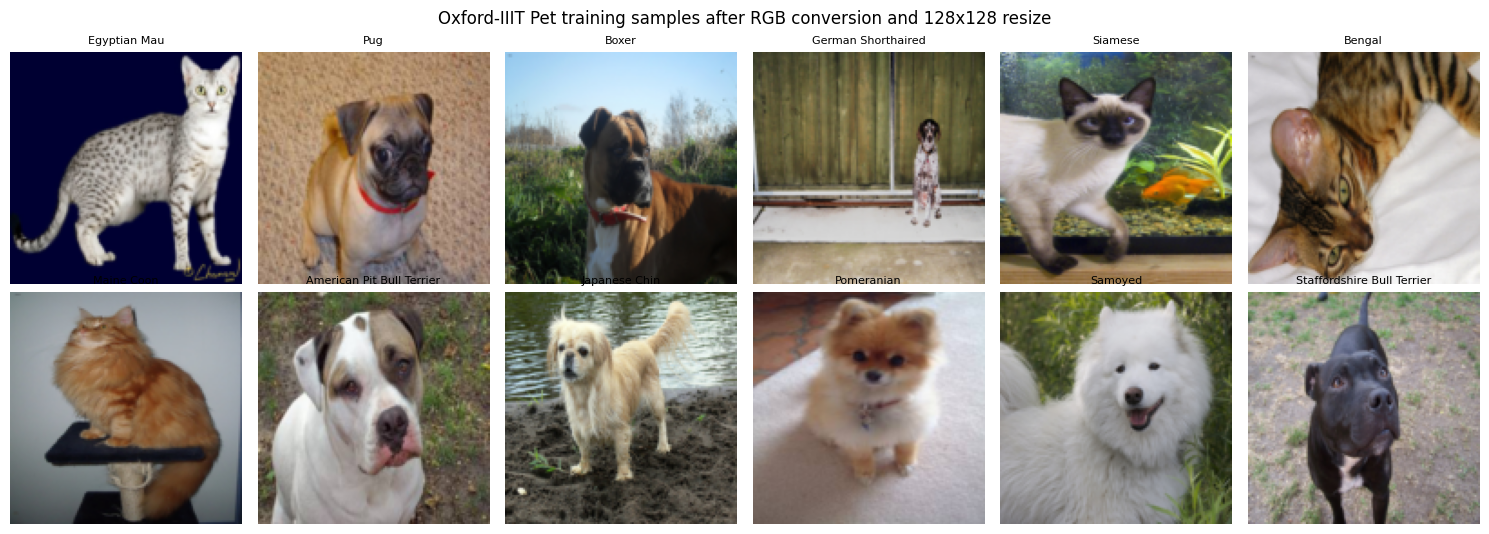
\includegraphics[width=0.49\textwidth]{data_samples.png}}\hfill
\subfloat[{\texttt{train\_ds[0]}} loaded eight times: a new corruption and severity on every load.]{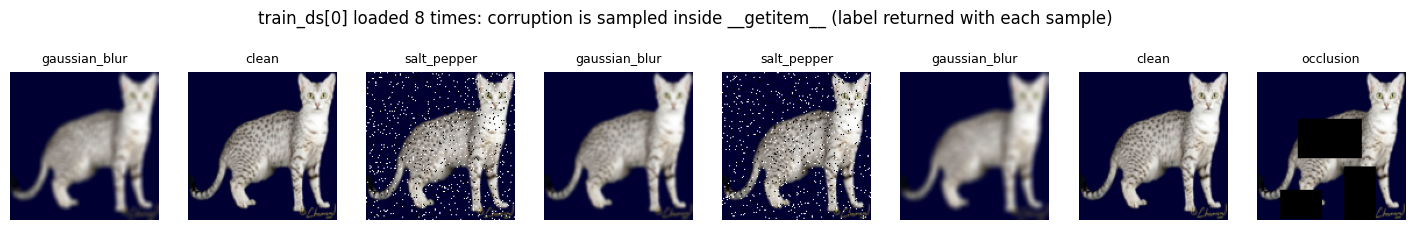
\includegraphics[width=0.49\textwidth]{data_runtime_corruption.png}}\\
\subfloat[Fixed test corruptions: every corruption $\times$ severity, taken from the deterministic manifest.]{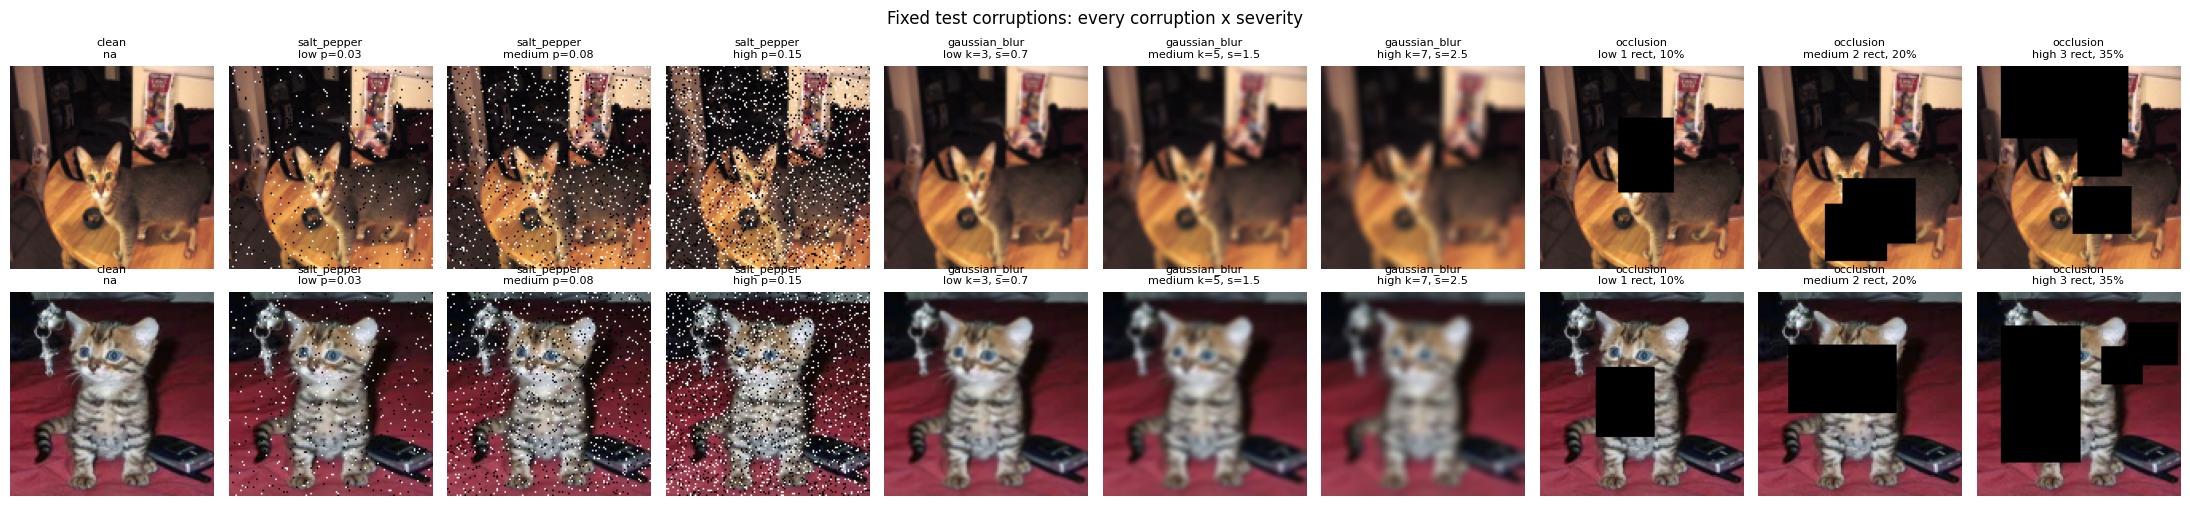
\includegraphics[width=\textwidth]{data_severity_grid.png}}
\caption{Dataset and corruption pipeline for Tasks 1--3.}
\label{fig:data}
\end{figure*}

\subsection{FS2K (Task 4)}
FS2K~\cite{fan2022fs2k} provides 2{,}104 photo--sketch pairs in three sketch styles with official train (1{,}058) and test (1{,}046) definitions. We hold out 15\% of the official training portion, stratified by style with seed~42 (\texttt{train\_test\_split}). This gives 899 training pairs (303/298/298 per style) and 159 validation pairs (54/52/53). The test set (619/381/46) is used only for final evaluation. The splits are disjoint. Pairs are resized to $128{\times}128$ and scaled to $[-1,1]$. Training augmentation draws one horizontal flip, one rotation angle in $[-8^\circ,8^\circ]$ and one resized-crop window per sample, and applies them identically to the photo and its sketch (Fig.~\ref{fig:t4data}).

%=====================================================================
\section{Experimental Setup}\label{sec:setup}
\textbf{Hardware and software.} All models were trained on Google Colab with an NVIDIA T4 GPU, using Python 3, PyTorch, \texttt{pytorch-msssim}, Optuna (TPE sampler, seed 42), MLflow and ONNX/ONNX Runtime. Checkpoints, manifests, Optuna studies and the MLflow store are kept on Google Drive, and every training loop resumes from its last checkpoint. Global seeds (Python, NumPy, PyTorch) are fixed to 42.

\textbf{Protocol.} Hyperparameters are chosen only on validation data. Optuna trials use short budgets, after which the selected configuration is retrained with early stopping on the validation objective. The best-validation checkpoint is reloaded and evaluated once on the untouched official test set: the 36{,}690-entry test manifest for Tasks 1--3, and the 1{,}046 official FS2K test pairs for Task 4.

\textbf{Metrics.}
\begin{itemize}
\item Restoration: per-image L1, SSIM (Gaussian window, data range 1) and PSNR $=10\log_{10}(1/\mathrm{MSE})$, averaged by corruption type and severity. PSNR is capped at 80\,dB when an output equals its target exactly.
\item Classifier: accuracy, macro and per-class precision/recall/F1, and a row-normalised confusion matrix.
\item Soft MoE: mean routing weight per type and severity.
\item Task 4: L1 (in $[-1,1]$ units), SSIM and PSNR on $[0,1]$ images, per style. We also measure style controllability and output diversity (mode-collapse ratio).
\item ONNX: maximum and mean absolute difference from PyTorch on real test images.
\end{itemize}

%=====================================================================
\section{Task 1: Universal Multi-Corruption Denoising Autoencoder}\label{sec:t1}
\subsection{Architecture}
The model $\hat x = D(E(\tilde x, c), c)$ (Fig.~\ref{fig:t1arch}) consists of three parts.
\begin{itemize}
\item \emph{Encoder.} A stem convolution, then four stride-2 $4{\times}4$ convolutions ($128{\to}64{\to}32{\to}16{\to}8$) with channels $c,2c,4c,8c,8c$, $c{=}64$, GroupNorm and ReLU. One FiLM residual block and dropout follow.
\item \emph{Bottleneck.} A $1{\times}1$ squeeze convolution produces the latent $z\in\mathbb{R}^{128\times8\times8}$: 8{,}192 values, 16.7\% of the 49{,}152-value input.
\item \emph{Decoder.} A $1{\times}1$ expansion, a FiLM residual block and four resize-convolution up-blocks, ending in a sigmoid RGB output.
\end{itemize}
A degradation encoder (three stride-2 convolutions and global pooling) produces a 64-d code $c$ from the corrupted image itself. This code sets the FiLM $(\gamma,\beta)$ parameters, which are initialised to identity. There are \emph{no} encoder--decoder skip connections: the decoder receives only $z$ and the global code $c$, which has no spatial layout and so cannot carry pixels around the bottleneck. Skips were deliberately not used, because they would copy noise and occlusion masks straight to the output. The model has 20.68\,M parameters: 0.11\,M in the degradation encoder, 11.81\,M in the encoder and 8.77\,M in the decoder.

\begin{figure}[!t]
\centering
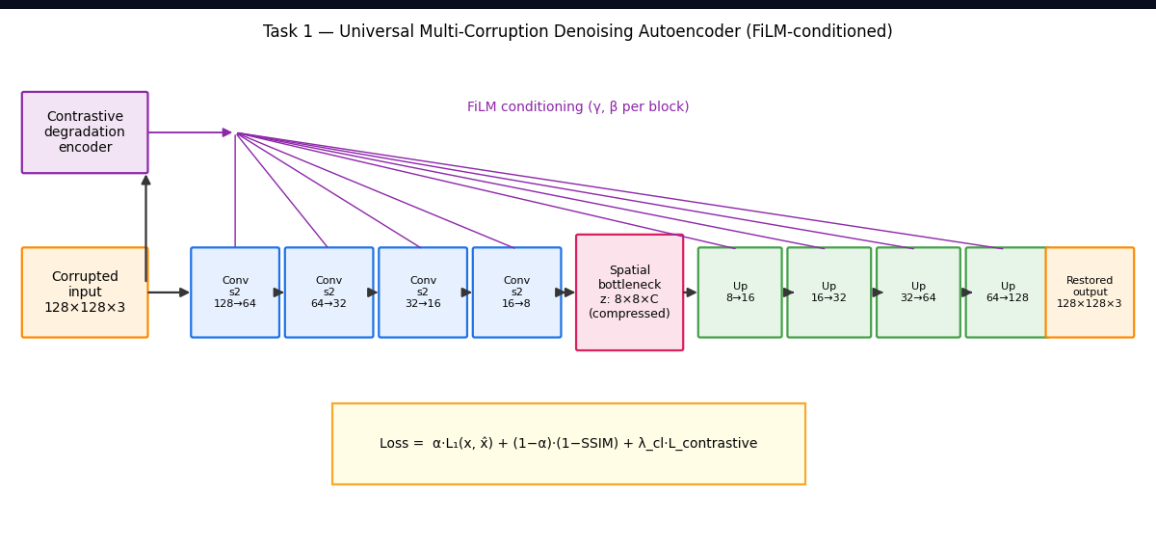
\includegraphics[width=\columnwidth]{t1_arch.png}
\caption{Task 1 architecture: contrastive degradation encoder, FiLM-conditioned convolutional encoder and decoder, and spatial bottleneck $z$ ($128{\times}8{\times}8$).}
\label{fig:t1arch}
\end{figure}

\subsection{Loss}
\begin{equation}
\mathcal{L}_{rec}=\alpha\,\lVert x-\hat x\rVert_1+(1-\alpha)\bigl(1-\ssim(x,\hat x)\bigr),\label{eq:rec}
\end{equation}
\begin{equation}
\mathcal{L}_{total}=\mathcal{L}_{rec}+\lambda_{cl}\,\mathcal{L}_{\text{NT-Xent}}(p_1,p_2),\label{eq:t1total}
\end{equation}
where $p_1,p_2$ are projections of two random $64{\times}64$ crops of the same corrupted image (positives). Crops of other images in the batch serve as negatives (temperature 0.2). Validation and model selection use $\mathcal{L}_{rec}$ only.

\subsection{Hyperparameter optimisation}
The Optuna search space covers learning rate, batch size, bottleneck channels, encoder base channels, residual blocks, dropout, $\alpha$, degradation-embedding dimension and $\lambda_{cl}$ (Table~\ref{tab:t1optuna}). Each trial trains for 4 epochs and is scored by its best validation $\mathcal{L}_{rec}$, which combines reconstruction error and SSIM. Sampling is TPE with seed 42, a median pruner removes weak trials, and the study is persisted to SQLite. Of 38 trials, 25 completed, 12 were pruned and 1 failed. The best value was 0.1157 (trial~1). Fig.~\ref{fig:t1optuna} shows the optimisation history and fANOVA importances. $\alpha$ dominates (importance 0.80), followed by dropout (0.06), residual blocks (0.05) and learning rate (0.04). Bottleneck width has importance below 0.01 in the range tested.

\begin{table}[!t]
\caption{Task 1 Optuna search space and selected configuration}
\label{tab:t1optuna}
\centering\footnotesize
\begin{tabular}{@{}lll@{}}
\toprule
Hyperparameter & Search range & Selected\\
\midrule
Learning rate & $[10^{-4},3{\times}10^{-3}]$ (log) & $2.69{\times}10^{-4}$\\
Batch size & \{32, 64, 128\} & 32\\
Bottleneck channels & \{64, 96, 128, 192\} & 128\\
Encoder base channels & \{24, 32, 48, 64\} & 64\\
Residual blocks & [1, 3] & 1\\
Dropout & [0, 0.3] & 0.0195\\
$\alpha$ (L1 weight) & [0.5, 0.95] & 0.927\\
Degradation embed. dim. & \{64, 128, 256\} & 64\\
$\lambda_{cl}$ & $[0.02,0.5]$ (log) & 0.0274\\
\bottomrule
\end{tabular}
\end{table}

\begin{figure}[!t]
\centering
\subfloat[Optimisation history.]{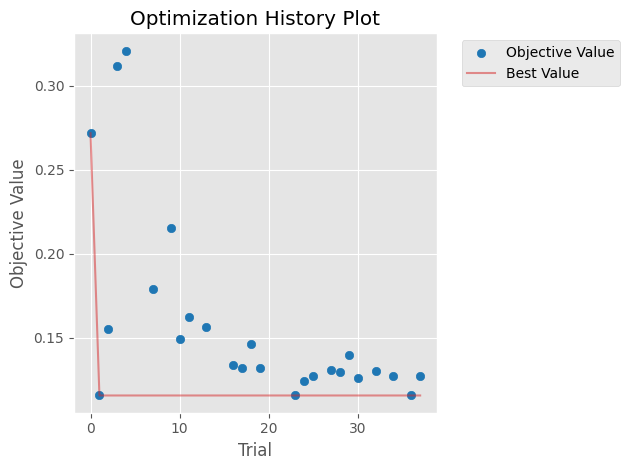
\includegraphics[width=0.49\columnwidth]{t1_optuna_history.png}}\hfill
\subfloat[Hyperparameter importance.]{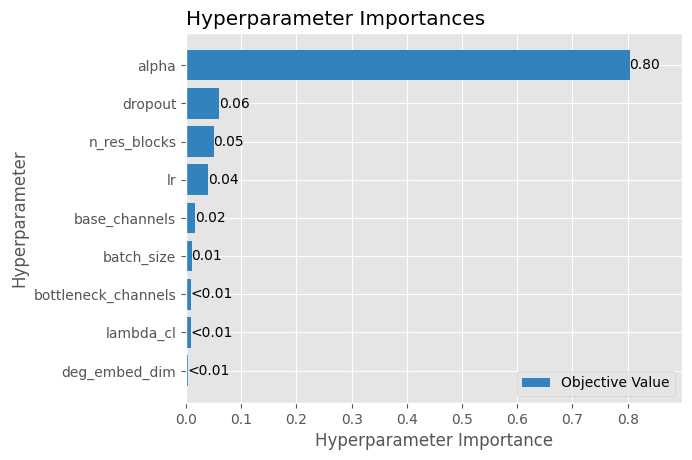
\includegraphics[width=0.49\columnwidth]{t1_optuna_importance.png}}
\caption{Task 1 Optuna study (38 trials: 25 complete, 12 pruned, 1 failed).}
\label{fig:t1optuna}
\end{figure}

\subsection{Training procedure}
The selected configuration was trained with Adam (learning rate $2.69{\times}10^{-4}$, batch 32) and ReduceLROnPlateau (factor 0.5, patience 4) for up to 60 epochs, with early-stopping patience 10. The best checkpoint was chosen by validation $\mathcal{L}_{rec}$. Fig.~\ref{fig:t1curves} shows the curves. Train and validation reconstruction losses fall together from $\approx$0.20/0.16 to $\approx$0.05. Validation SSIM rises from 0.40 to 0.78, and the contrastive loss falls from 2.85 to 1.25. The train and validation curves never diverge, so there is no overfitting. Validation SSIM is still rising slowly at epoch 60, which indicates the model is budget-limited rather than capacity-limited.

\begin{figure*}[!t]
\centering
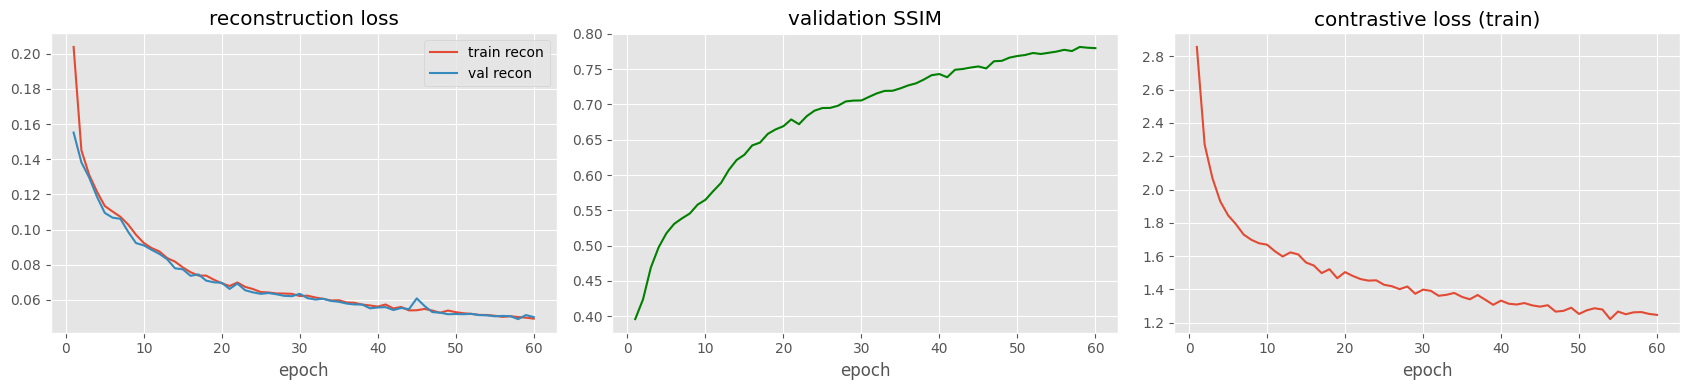
\includegraphics[width=0.9\textwidth]{t1_training_curves.png}
\caption{Task 1 training curves: reconstruction loss (train/validation), validation SSIM and contrastive loss over the 60-epoch run.}
\label{fig:t1curves}
\end{figure*}

\subsection{Results}
Table~\ref{tab:t1res} reports L1, SSIM and PSNR on the 36{,}690-entry test manifest by corruption and severity.

\emph{Important caveat.} The checkpoint available for this evaluation does not match the training run in Fig.~\ref{fig:t1curves}. Its test SSIM (0.40--0.41 on all non-occluded conditions) equals the \emph{epoch-1} validation SSIM of the run. Its outputs are nearly identical across clean, noisy and blurred inputs (Fig.~\ref{fig:t1ex}), and its metadata label (``epoch 10, val.\ loss 0.0869'') is inconsistent with this measured performance. The best checkpoint was overwritten during a checkpoint-synchronisation step between Colab sessions. Without retraining, the numbers in Table~\ref{tab:t1res} therefore describe an early-epoch model; the logged run reached validation SSIM 0.78. Even this early model shows the expected pattern: occlusion is clearly the hardest corruption, and its error grows monotonically with severity (SSIM $0.392{\to}0.377{\to}0.357$).

\begin{table}[!t]
\caption{Task 1 test results by corruption type and severity (evaluated checkpoint)}
\label{tab:t1res}
\centering\footnotesize
\begin{tabular}{@{}llccc@{}}
\toprule
Type & Severity & L1$\downarrow$ & SSIM$\uparrow$ & PSNR (dB)$\uparrow$\\
\midrule
Clean & -- & 0.1151 & 0.4060 & 16.80\\
\multirow{3}{*}{Salt-and-pepper} & low & 0.1149 & 0.4060 & 16.82\\
 & medium & 0.1147 & 0.4058 & 16.84\\
 & high & 0.1149 & 0.4050 & 16.84\\
\multirow{3}{*}{Gaussian blur} & low & 0.1152 & 0.4058 & 16.79\\
 & medium & 0.1153 & 0.4055 & 16.79\\
 & high & 0.1154 & 0.4050 & 16.79\\
\multirow{3}{*}{Occlusion} & low & 0.1223 & 0.3918 & 16.19\\
 & medium & 0.1318 & 0.3772 & 15.47\\
 & high & 0.1472 & 0.3565 & 14.44\\
\midrule
\multicolumn{2}{@{}l}{All conditions pooled} & 0.1207 & 0.3965 & 16.38\\
\bottomrule
\end{tabular}
\end{table}

\begin{figure}[!t]
\centering
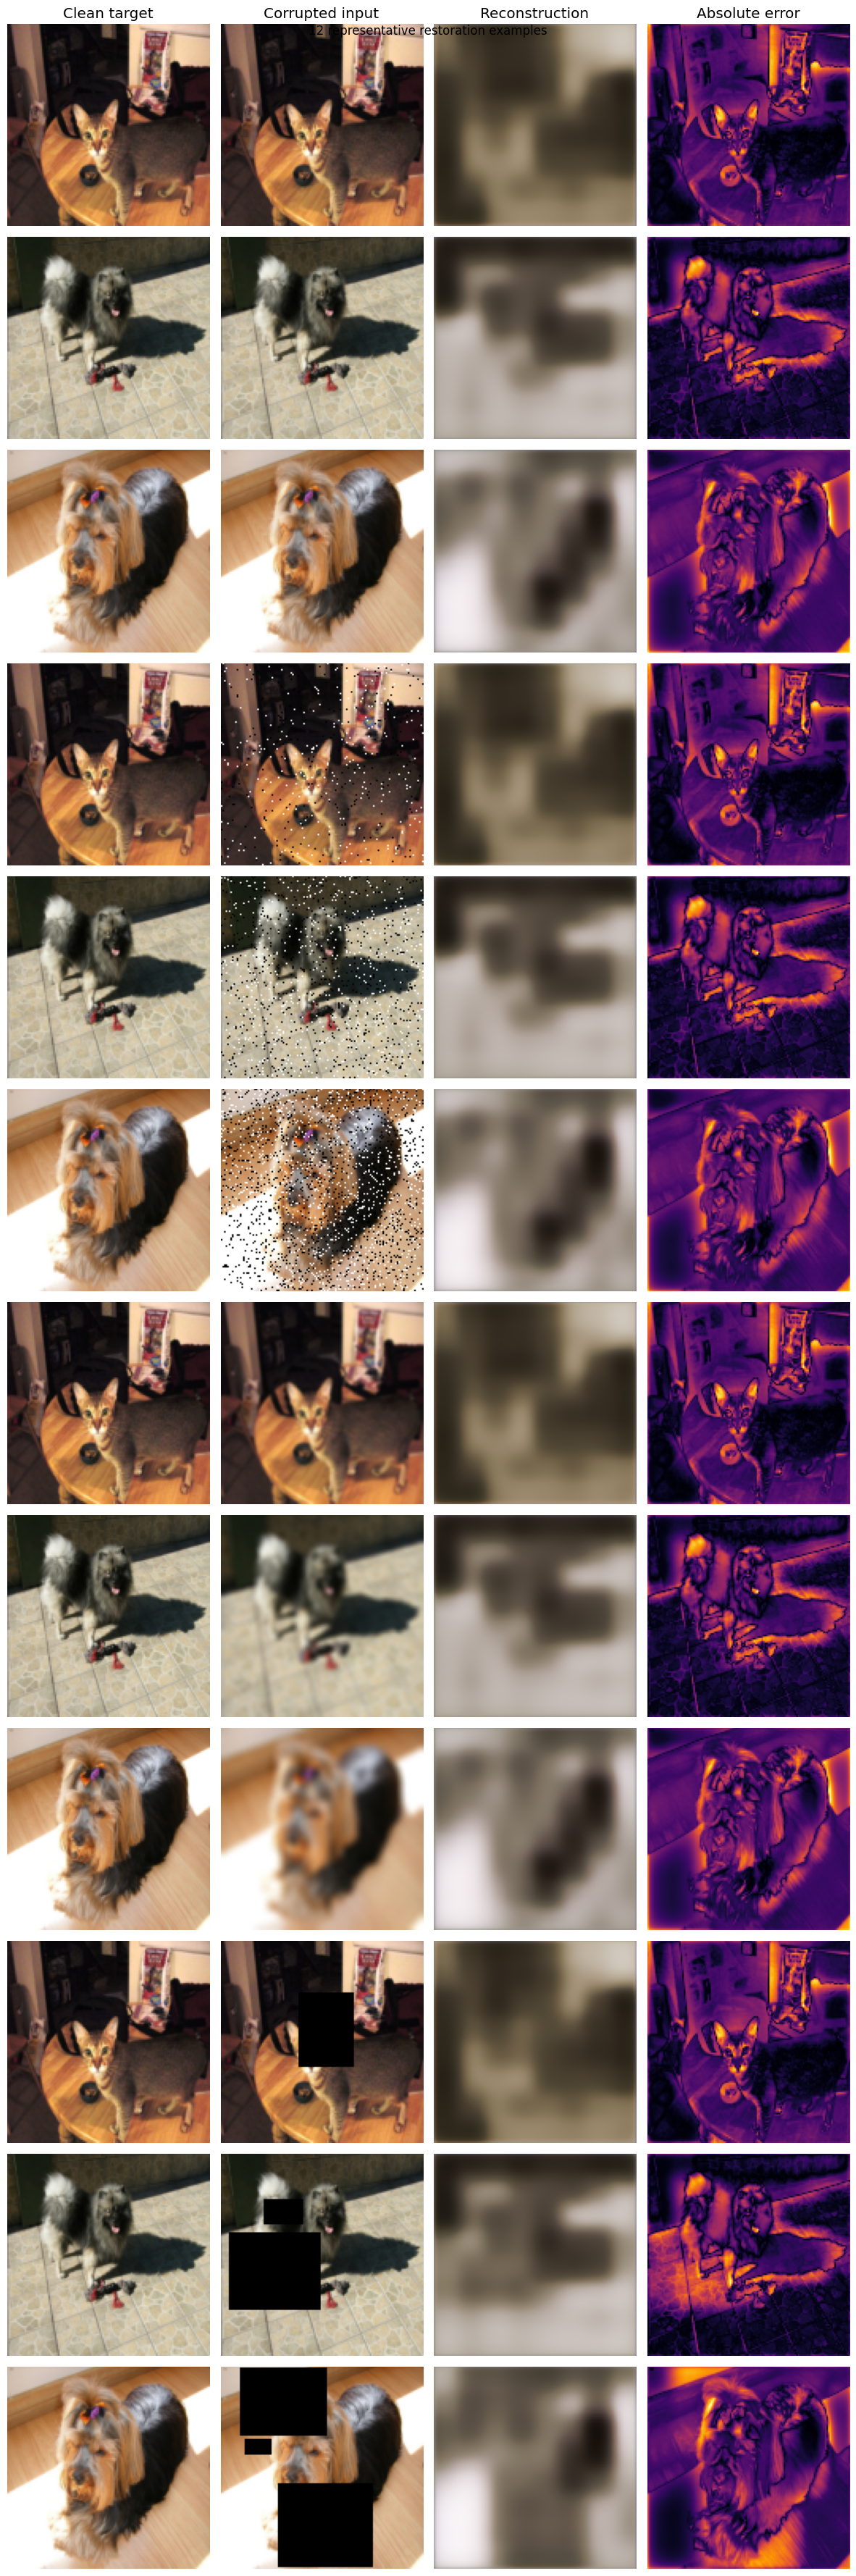
\includegraphics[height=0.86\textheight]{t1_examples12.png}
\caption{Twelve representative Task 1 test examples (3 clean, 3 salt-and-pepper, 3 blur, 3 occlusion). Columns: clean target, corrupted input, reconstruction, absolute error map.}
\label{fig:t1ex}
\end{figure}

\begin{figure}[!t]
\centering
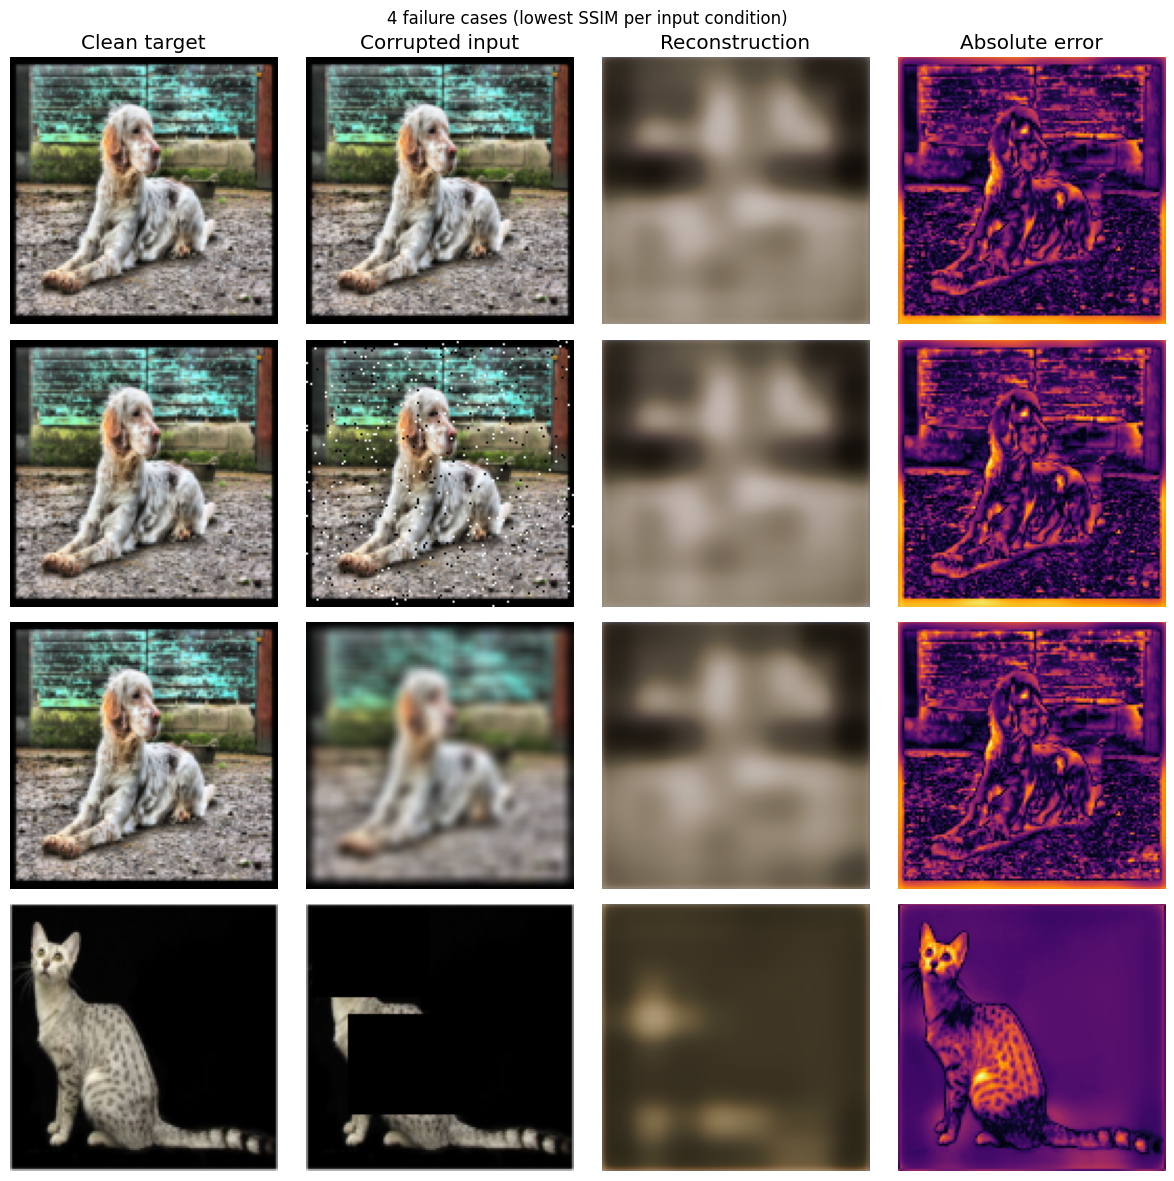
\includegraphics[width=\columnwidth]{t1_failures.png}
\caption{Task 1 failure cases: the lowest-SSIM sample of each input condition (clean SSIM 0.103, salt-and-pepper 0.103, blur 0.099, occlusion 0.074), with absolute error maps.}
\label{fig:t1fail}
\end{figure}

\subsection{Failure analysis and discussion}
Fig.~\ref{fig:t1ex} shows twelve examples with error maps, and Fig.~\ref{fig:t1fail} the worst case of each condition.
\begin{itemize}
\item \emph{(i) Highly textured images.} The three worst non-occlusion cases are the same image: a dog on gravel in front of a brick wall, with a black frame. Its fine, high-contrast texture cannot pass through an $8{\times}8$ latent, and the error map lights up on every texture edge and along the frame.
\item \emph{(ii) Large occlusions on dark backgrounds.} The worst occlusion case (SSIM 0.074) hides most of a cat on a black background. The reconstruction is a low-contrast mean colour, and the error concentrates on the masked animal.
\item \emph{(iii) Clean inputs.} Clean images lose quality because a universal autoencoder has no identity path. This is the main motivation for the identity bypass in Tasks~2 and~3.
\end{itemize}
Design lessons: the spatial bottleneck and resize-convolution decoder removed the blur and checkerboard artifacts of earlier versions. Optuna's strong preference for a large L1 weight ($\alpha{=}0.93$) favours colour fidelity over structural sharpness. A single universal model must denoise, deblur and inpaint with one set of weights, which limits it on every individual task.

%=====================================================================
\section{Task 2: Corruption Classification and Hard-Routed Specialists}\label{sec:t2}
\subsection{Corruption classifier}
$C(\tilde x)$ is a five-stage CNN: stride-2 $3{\times}3$ convolutions with channels $16\cdot2^i$, GroupNorm and ReLU, followed by global average pooling, dropout and a linear layer. It outputs four logits, giving $p=\mathrm{softmax}(C(\tilde x))$ and the route $r=\arg\max_k p_k$. Training minimises multiclass cross-entropy with labels produced by the corruption pipeline. Batches are \emph{exactly} balanced: the class of training index $i$ is fixed to $i \bmod 4$ while the image and severity are re-sampled on every access, and with an unshuffled loader each batch of 32 holds 8 samples per class (verified on the first five batches). The Optuna search covered learning rate, batch size, depth and base width (the channel configuration), dropout and weight decay. It ran 20 trials (13 complete, 7 pruned, 3 epochs each, objective validation cross-entropy; Fig.~\ref{fig:t2optuna}a) and selected learning rate $6.38{\times}10^{-4}$, batch 32, 5 layers, width 16, dropout 0.381 and weight decay $1.02{\times}10^{-4}$. The final classifier (0.39\,M parameters) was trained with AdamW for 30 epochs (best validation loss 0.0461). Training and validation curves track each other at $\approx$98\% accuracy (Fig.~\ref{fig:t2clf}a).

\begin{figure*}[!t]
\centering
\subfloat[Classifier study (20 trials).]{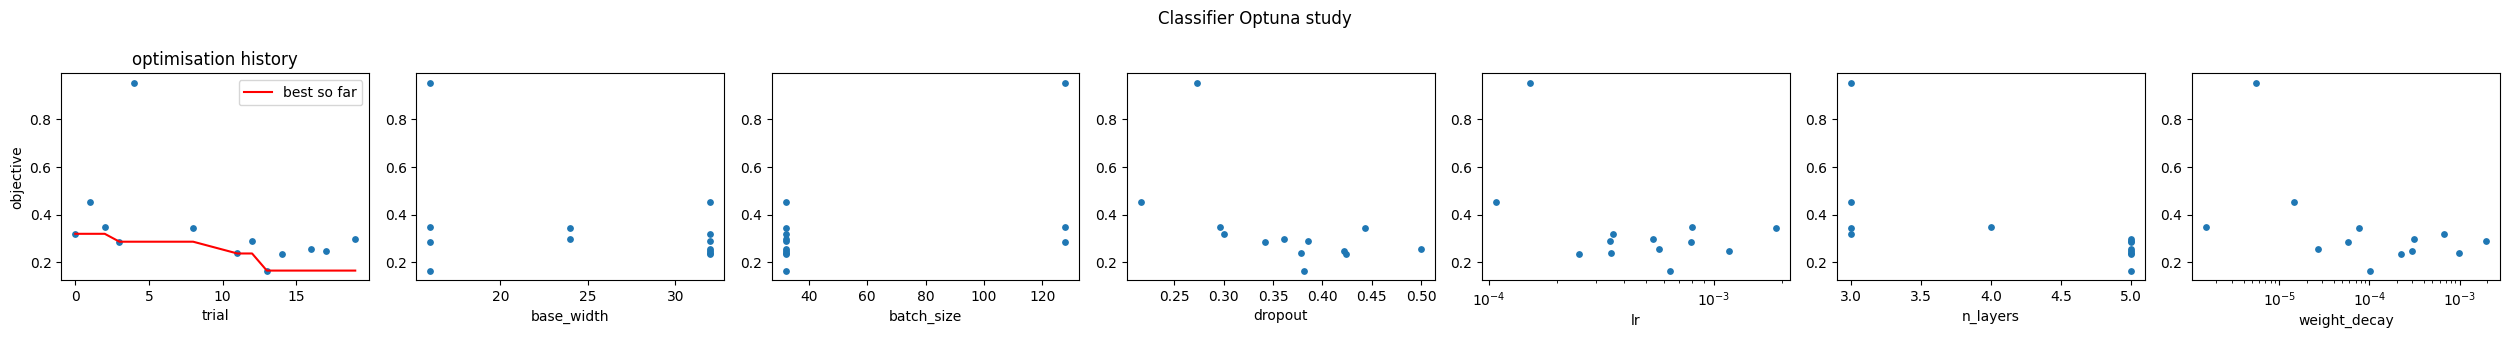
\includegraphics[width=\textwidth]{t2_optuna_classifier.png}}\\
\subfloat[Shared specialist study (20 trials, blur specialist as proxy).]{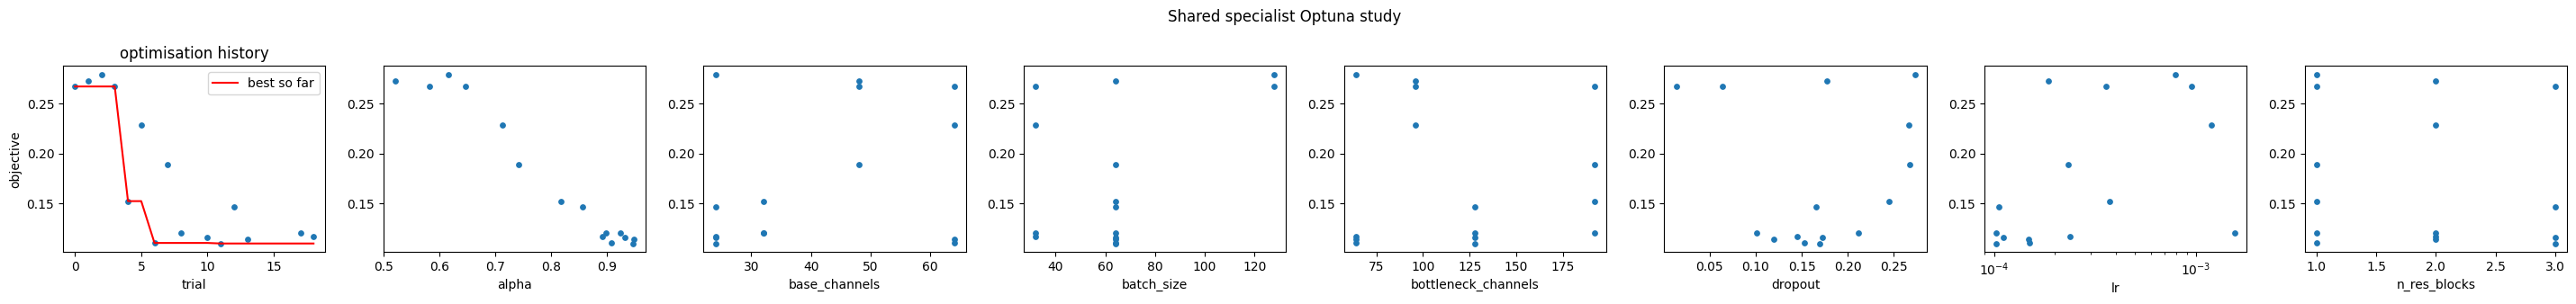
\includegraphics[width=\textwidth]{t2_optuna_specialists.png}}
\caption{Task 2 Optuna studies: optimisation history (red: best so far) and objective versus each hyperparameter.}
\label{fig:t2optuna}
\end{figure*}

\begin{table}[!t]
\caption{Corruption classifier on the test manifest (36{,}690 inputs)}
\label{tab:t2clf}
\centering\footnotesize
\begin{tabular}{@{}lcccr@{}}
\toprule
Class & Precision & Recall & F1 & Support\\
\midrule
Clean & 0.862 & 0.988 & 0.921 & 3{,}669\\
Salt-and-pepper & 1.000 & 1.000 & 1.000 & 11{,}007\\
Gaussian blur & 0.996 & 0.963 & 0.979 & 11{,}007\\
Occlusion & 0.999 & 0.983 & 0.991 & 11{,}007\\
\midrule
Macro average & 0.964 & 0.984 & 0.973 & 36{,}690\\
\multicolumn{5}{@{}l}{Overall accuracy: 0.9827}\\
\bottomrule
\end{tabular}
\end{table}

\begin{figure}[!t]
\centering
\subfloat[Training curves.]{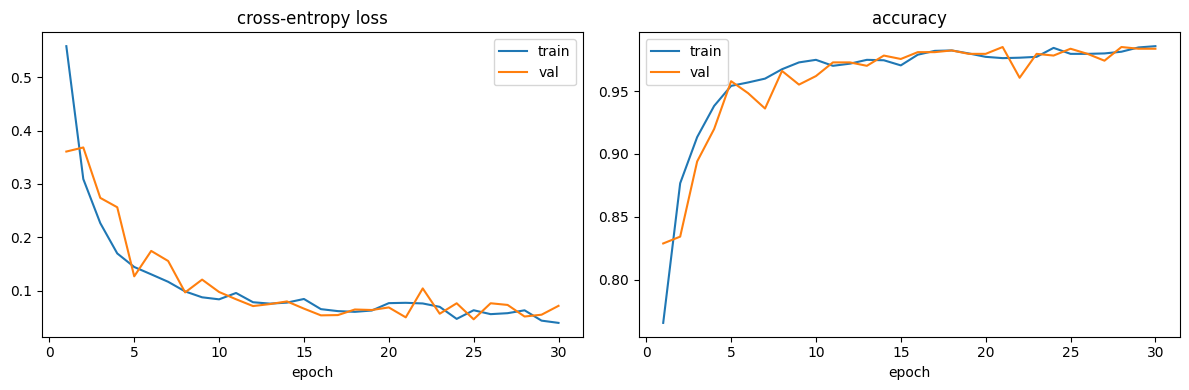
\includegraphics[width=\columnwidth]{t2_classifier_curves.png}}\\
\subfloat[Row-normalised confusion matrix (test).]{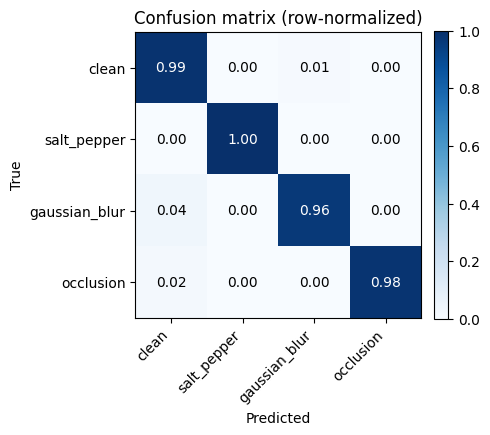
\includegraphics[width=0.62\columnwidth]{t2_confusion_matrix.png}}
\caption{Task 2 corruption classifier.}
\label{fig:t2clf}
\end{figure}

Table~\ref{tab:t2clf} and Fig.~\ref{fig:t2clf}b report the test performance. Salt-and-pepper is never confused, because isolated pure black and white pixels are unique to it. Almost every error is a corrupted image predicted as \emph{clean}: 404 blurred images, all at low severity ($k{=}3$, $\sigma{=}0.7$, a very slight softening at $128{\times}128$), and 176 occlusions whose rectangles fall on naturally dark regions such as black fur or shadow. This is why clean has recall 0.988 but precision 0.862. Corrupted classes are almost never confused with each other (only 11 blur$\leftrightarrow$occlusion errors).

\subsection{Specialist autoencoders}
The three specialists share one architecture: the Task 1 backbone without degradation conditioning, with a spatial $128{\times}8{\times}8$ bottleneck and no skips. Each has 5.57\,M parameters but independently trained weights and a different initialisation seed. Each sees \emph{only} its own corruption during training, with the clean image as the target. One shared Optuna search, using the blur specialist as a proxy because deblurring needs the most high-frequency reconstruction, tuned learning rate, batch size, bottleneck size, base channels, residual blocks, dropout and the L1/SSIM weight $\alpha$. It ran 20 trials (15 complete, 5 pruned; Fig.~\ref{fig:t2optuna}b) and selected learning rate $1.03{\times}10^{-4}$, batch 64, bottleneck 128, base 24, 3 residual blocks, dropout 0.17 and $\alpha{=}0.947$. Dropout was searched in $[0,0.3]$, and the code range was tightened to $[0,0.15]$ only afterwards. In addition to Eq.~\eqref{eq:rec}, the blur specialist adds a Sobel edge loss (weight 0.15), which penalises residual softness. The occlusion specialist adds a VGG-16 perceptual loss~\cite{johnson2016perceptual} (weight 0.10), which discourages flat fills~\cite{pathak2016}. Each specialist was trained with Adam and ReduceLROnPlateau for up to 200 epochs (patience 25), validated on a dedicated full-size validation manifest for its corruption. The best validation losses were 0.057 (salt-and-pepper), 0.099 (blur) and 0.323 (occlusion, which includes the perceptual term). Fig.~\ref{fig:t2spec} shows the curves. Salt-and-pepper and blur converge by $\approx$150 epochs (validation SSIM $\approx$0.71--0.72). Occlusion is still improving at epoch 200 (validation SSIM $\approx$0.65).

\begin{figure*}[!t]
\centering
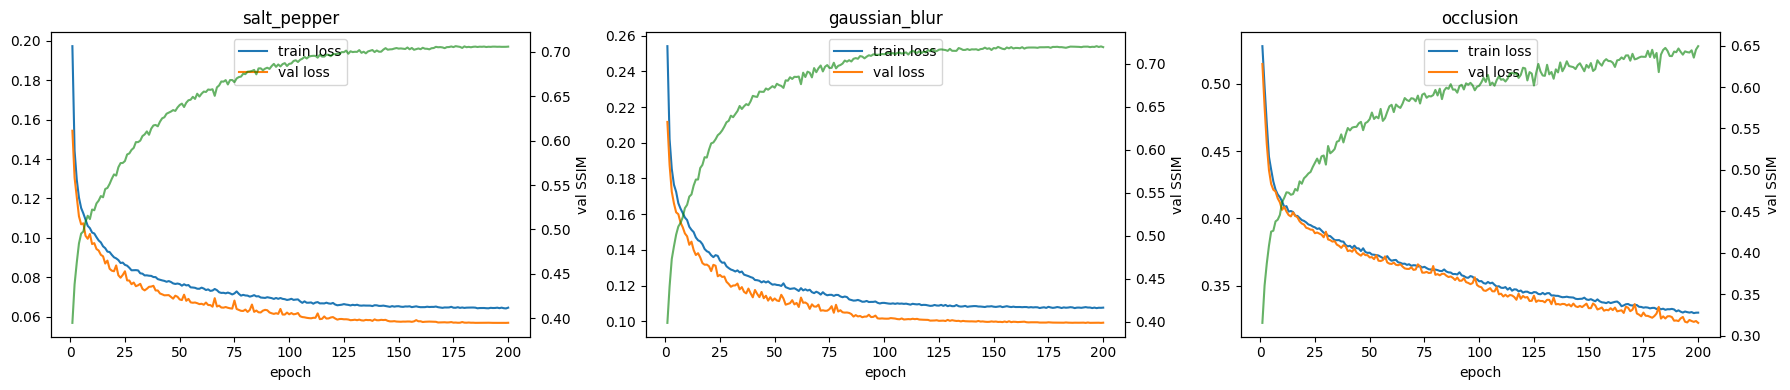
\includegraphics[width=0.92\textwidth]{t2_specialist_curves.png}
\caption{Training/validation loss (left axis) and validation SSIM (right axis, green) of the three specialists.}
\label{fig:t2spec}
\end{figure*}

\subsection{Hard-routed inference}
\begin{equation}
\hat x=\begin{cases}\tilde x & r=\text{clean (identity bypass)}\\ A_{salt}(\tilde x) & r=\text{salt}\\ A_{blur}(\tilde x) & r=\text{blur}\\ A_{occ}(\tilde x) & r=\text{occlusion}\end{cases}
\end{equation}
Clean predictions skip all experts (Fig.~\ref{fig:t2arch}). In \emph{oracle} mode the manifest label selects the expert; in \emph{predicted} mode the classifier does. Table~\ref{tab:t2route} lists both by corruption and severity. The oracle columns are each specialist's own performance on its corruption at each severity level. Oracle and predicted routing are identical on every salt-and-pepper, medium/high-blur and most occlusion inputs. Predicted routing is even \emph{better} on low blur (SSIM 0.755 vs 0.721) and low occlusion (0.696 vs 0.688). In these cases the misrouted inputs are barely corrupted, so the identity bypass keeps them closer to the target than the specialist reconstruction does. On clean inputs predicted routing loses 0.0023 SSIM, because 45 clean images (1.2\%) were sent to an expert. Pooled over all 36{,}690 inputs, SSIM is 0.718 (oracle) and 0.723 (predicted).

\begin{figure}[!t]
\centering
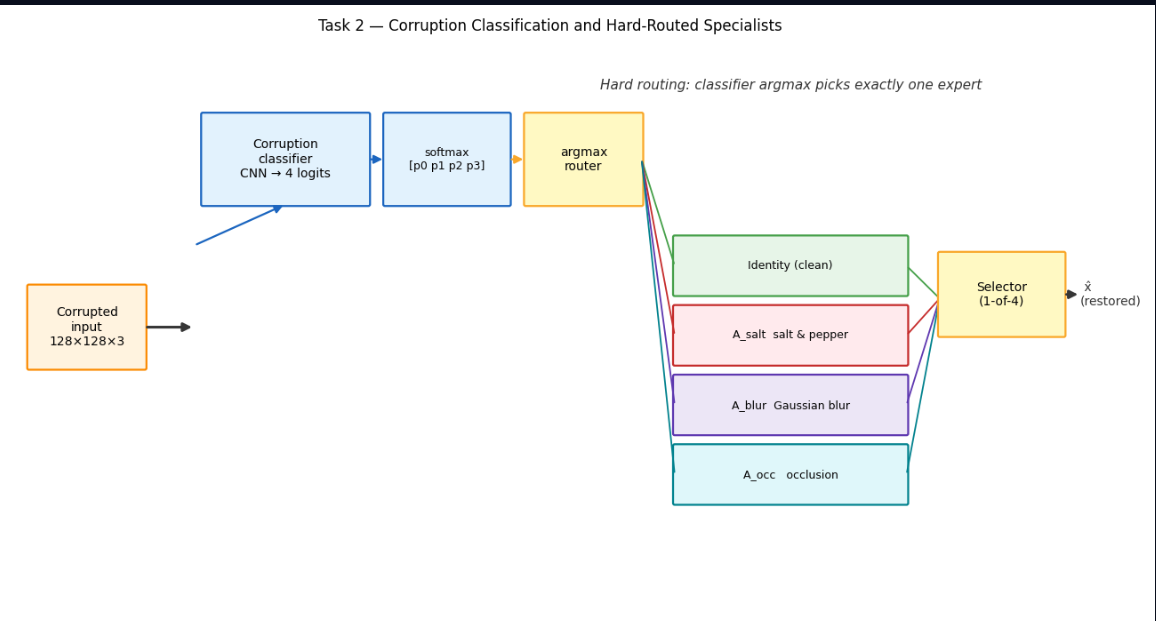
\includegraphics[width=\columnwidth]{t2_arch.png}
\caption{Task 2 architecture: the classifier's argmax selects exactly one branch (identity bypass or one specialist).}
\label{fig:t2arch}
\end{figure}

\begin{table}[!t]
\caption{Hard routing on the test set: oracle vs predicted routing, and comparison with Task 1 (SSIM; PSNR in dB)}
\label{tab:t2route}
\centering\footnotesize
\setlength{\tabcolsep}{3pt}
\begin{tabular}{@{}llccccc@{}}
\toprule
 & & \multicolumn{3}{c}{SSIM$\uparrow$} & \multicolumn{2}{c}{PSNR$\uparrow$}\\
\cmidrule(lr){3-5}\cmidrule(l){6-7}
Type & Sev. & Task 1 & Oracle & Pred. & Oracle & Pred.\\
\midrule
Clean & -- & 0.406 & 1.000 & 0.998 & 80.0$^\ast$ & 79.4$^\ast$\\
\multirow{3}{*}{S\&P} & low & 0.406 & 0.706 & 0.706 & 24.24 & 24.24\\
 & med. & 0.406 & 0.703 & 0.703 & 24.20 & 24.20\\
 & high & 0.405 & 0.695 & 0.695 & 24.05 & 24.05\\
\multirow{3}{*}{Blur} & low & 0.406 & 0.721 & 0.755 & 24.38 & 25.34\\
 & med. & 0.406 & 0.716 & 0.716 & 24.43 & 24.43\\
 & high & 0.405 & 0.695 & 0.695 & 24.09 & 24.09\\
\multirow{3}{*}{Occl.} & low & 0.392 & 0.688 & 0.696 & 22.72 & 22.62\\
 & med. & 0.377 & 0.654 & 0.655 & 21.47 & 21.47\\
 & high & 0.357 & 0.607 & 0.607 & 19.94 & 19.94\\
\bottomrule
\multicolumn{7}{@{}l}{\scriptsize $^\ast$PSNR of an unchanged image is capped at 80\,dB (MSE$=0$).}
\end{tabular}
\end{table}

\subsection{Classifier-induced failures}
636 test inputs (1.73\%) are misrouted (Fig.~\ref{fig:t2fail}). Their mean SSIM (0.908) is \emph{higher} than that of correctly routed inputs (0.719), because only the mildest corruptions get misrouted. Two failure modes matter.
\begin{itemize}
\item \emph{Occlusion predicted as clean} (176 cases). The black rectangle survives unchanged (row 2).
\item \emph{Clean image predicted as blur} (37 cases). The image is needlessly passed through the blur specialist and loses detail (row 3).
\end{itemize}
The cheapest error is a low-severity blur sent to the bypass (rows 1 and 4), where the output keeps a slight softness but avoids the specialist's own smoothing. Fig.~\ref{fig:t2pipe} shows the complete operational pipeline on test images, as displayed by the application.

\begin{figure}[!t]
\centering
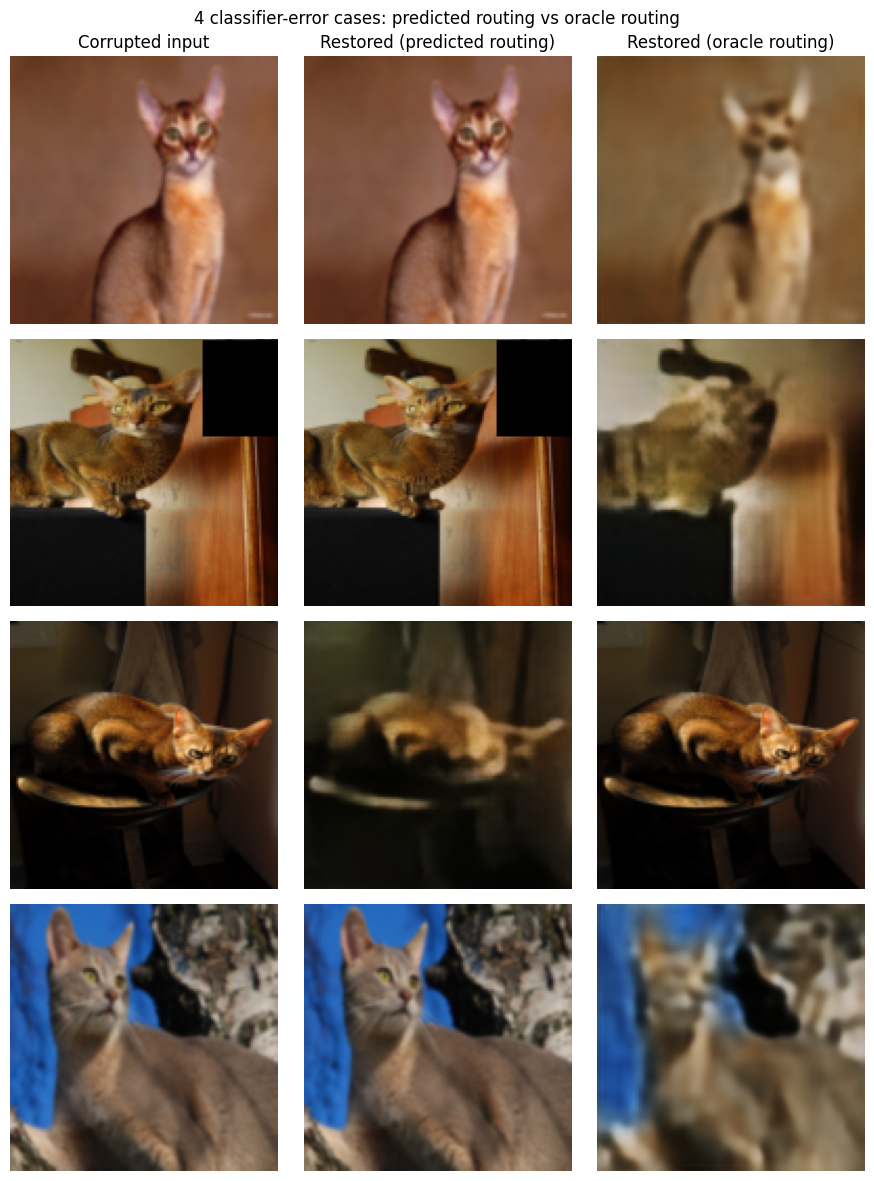
\includegraphics[width=0.9\columnwidth]{t2_misrouting.png}
\caption{Classifier errors that change the restoration: corrupted input, output under predicted routing, output under oracle routing.}
\label{fig:t2fail}
\end{figure}

\subsection{Comparison with Task 1}
Fig.~\ref{fig:t2vs1} and Table~\ref{tab:t2route} show that the specialists beat the evaluated Task 1 checkpoint on every condition, by about $+0.29$ SSIM and $+7.4$\,dB PSNR on salt-and-pepper and blur. Specialists help because each learns one inverse mapping and clean images bypass restoration entirely. They fail when the classifier is wrong and when an input mixes corruptions, because only one expert is ever applied. Part of the gap is also due to the early-epoch Task 1 checkpoint (Sec.~\ref{sec:t1}): the Task 1 training run reached validation SSIM 0.78. The ONNX exports reproduce PyTorch with maximum absolute differences of $8.1{\times}10^{-6}$ (classifier logits, 100\% argmax agreement) and $2.6{\times}10^{-5}$, $2.1{\times}10^{-5}$ and $2.1{\times}10^{-5}$ (salt-and-pepper, blur and occlusion specialists) on 32 test images.

\begin{figure*}[!t]
\centering
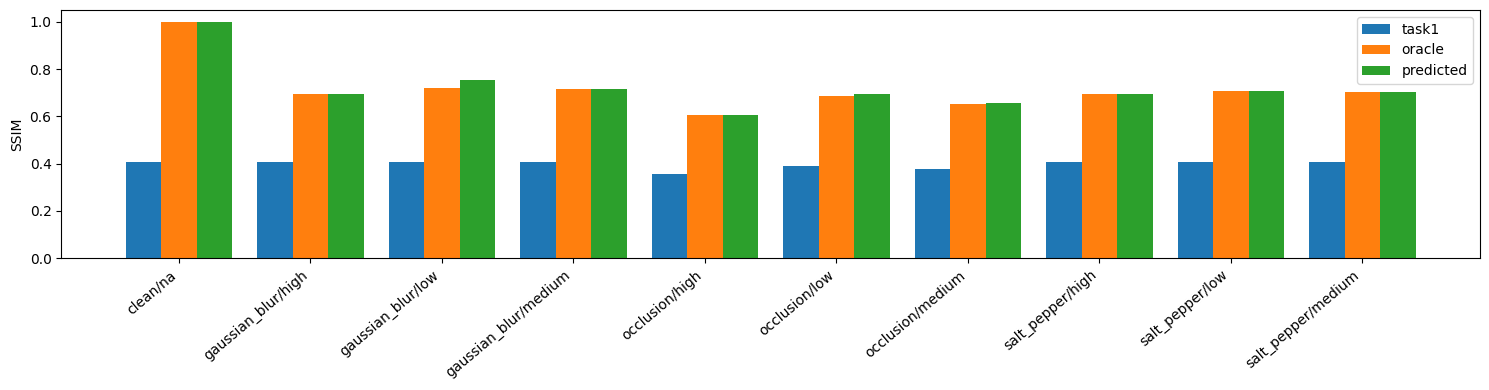
\includegraphics[width=0.9\textwidth]{t2_vs_t1.png}
\caption{Test SSIM by corruption/severity: Task 1 universal autoencoder (evaluated checkpoint) vs Task 2 oracle and predicted hard routing.}
\label{fig:t2vs1}
\end{figure*}

\begin{figure}[!t]
\centering
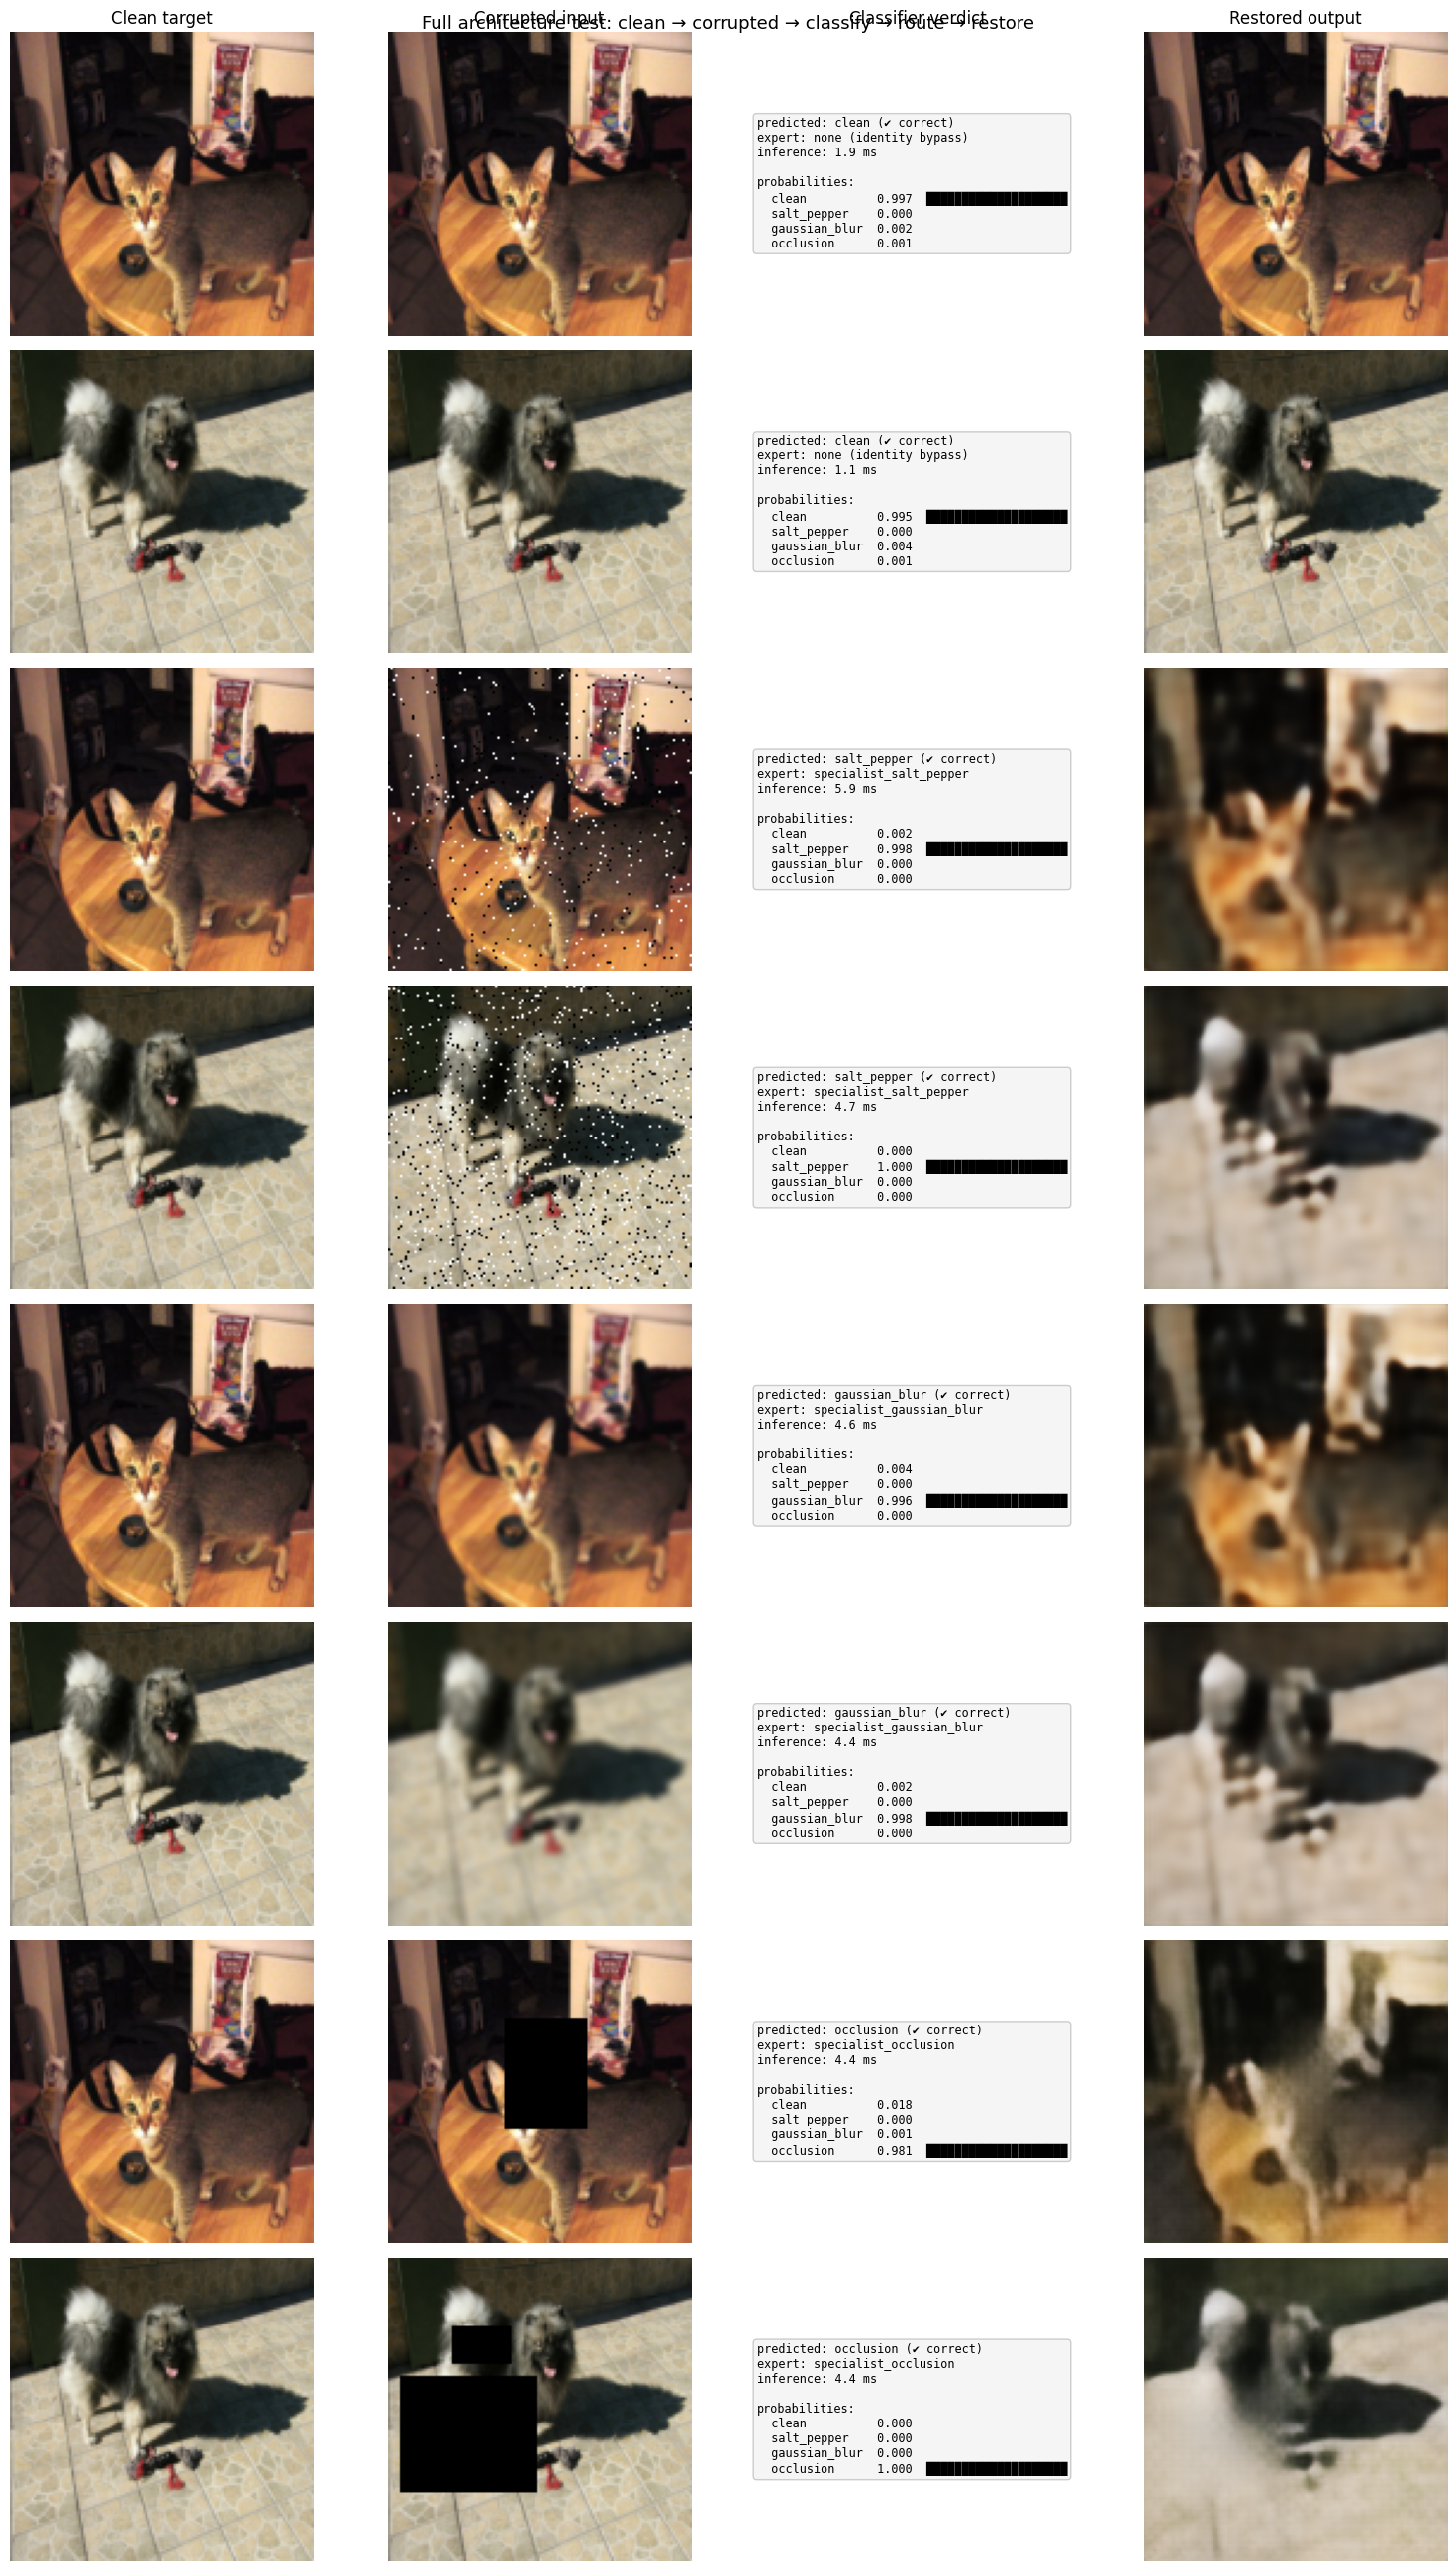
\includegraphics[width=\columnwidth]{t2_pipeline_examples.png}
\caption{End-to-end hard routing reloaded from the saved checkpoints: clean target, corrupted input, classifier verdict (four probabilities, predicted class, selected expert, inference time), restored output.}
\label{fig:t2pipe}
\end{figure}

%=====================================================================
\section{Task 3: Jointly Trained Soft Mixture of Experts}\label{sec:t3}
\subsection{Architecture}
The gate $G$, initialised from the Task 2 classifier, produces temperature-scaled weights over four branches (Fig.~\ref{fig:t3arch}):
\begin{equation}
w=\mathrm{softmax}\bigl(G(\tilde x)/\tau\bigr),\quad w=[w_0,w_1,w_2,w_3],
\end{equation}
\begin{equation}
\hat x=w_0\tilde x+w_1A_{salt}(\tilde x)+w_2A_{blur}(\tilde x)+w_3A_{occ}(\tilde x).
\end{equation}
The experts are initialised from the three Task 2 specialists, and $w_0$ weights an identity branch. The weighted sum is differentiable, so the reconstruction loss trains both the gate and the experts. The system has 17.1\,M parameters (gate 0.39\,M and $3\times5.57$\,M).

\begin{figure}[!t]
\centering
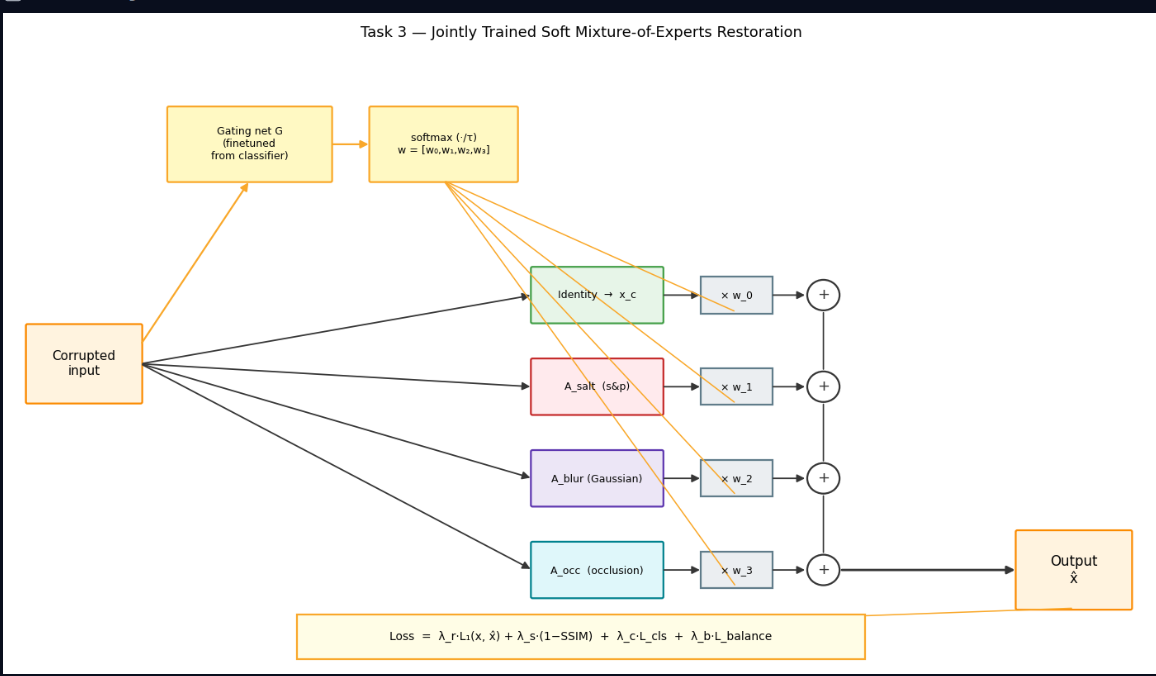
\includegraphics[width=\columnwidth]{t3_arch.png}
\caption{Task 3 soft mixture of experts: a gate (initialised from the Task 2 classifier) weights the identity branch and three experts (initialised from the Task 2 specialists).}
\label{fig:t3arch}
\end{figure}

\subsection{Joint loss and training}
\begin{equation}
\mathcal{L}_{MoE}=\lambda_1\mathrm{L1}+\lambda_2(1-\ssim)+\lambda_c\,\mathrm{CE}\bigl(G(\tilde x),y\bigr)+\lambda_b\,\mathcal{L}_{bal},
\end{equation}
\begin{equation}
\mathcal{L}_{bal}=\sum_{k=0}^{3}\Bigl(\bar w_k-\tfrac14\Bigr)^2,
\end{equation}
with $\lambda_1{=}\alpha$, $\lambda_2{=}1-\alpha$ and $\bar w_k$ the batch-mean weight of branch $k$. Batches are exactly class-balanced ($i\bmod4$), so a uniform batch-average target of $\tfrac14$ is correct even though individual images should be routed sharply. This is the load-balancing principle of sparse MoE~\cite{shazeer2017,fedus2022switch}. We rejected a per-sample entropy penalty, because it would push unambiguous inputs towards a uniform mixture. The cross-entropy term keeps $G$ tied to the runtime corruption label, which is used only during training.

\emph{Warm-up.} For 10 epochs only the gate is trained (Adam, learning rate $10^{-3}$, $\tau{=}1$, $\alpha{=}0.8$, $\lambda_c{=}0.1$, $\lambda_b{=}0.01$), and the experts stay frozen at their Task 2 weights. After warm-up the mean validation weights were 0.256/0.272/0.253/0.219, so no branch collapsed.

\emph{Joint fine-tuning.} All parameters are unfrozen and trained with the Optuna-selected learning rate of $1.61{\times}10^{-5}$, 62$\times$ smaller than in warm-up, for 60 epochs (patience 15). Fig.~\ref{fig:t3curves} shows validation loss falling from 0.052 to 0.049 and validation SSIM rising from 0.783 to 0.802, while gate accuracy stays at 97.5--98.4\%.

\emph{Optuna.} The search covered the joint learning rate, $\tau$, $\alpha$, $\lambda_c$ and $\lambda_b$ (Fig.~\ref{fig:t3optuna}). It ran 15 trials of 3 epochs, each starting from the post-warm-up checkpoint. Trials were pruned by the median pruner \emph{and} on routing collapse (any branch's mean weight $<0.02$ or $>0.9$): 7 completed and 8 were pruned. Selected: learning rate $1.61{\times}10^{-5}$, $\tau{=}1.692$, $\alpha{=}0.923$, $\lambda_c{=}0.0399$, $\lambda_b{=}0.00126$.

\begin{figure*}[!t]
\centering
\subfloat[Optuna study (15 trials; 8 pruned, including routing collapse).\label{fig:t3optuna}]{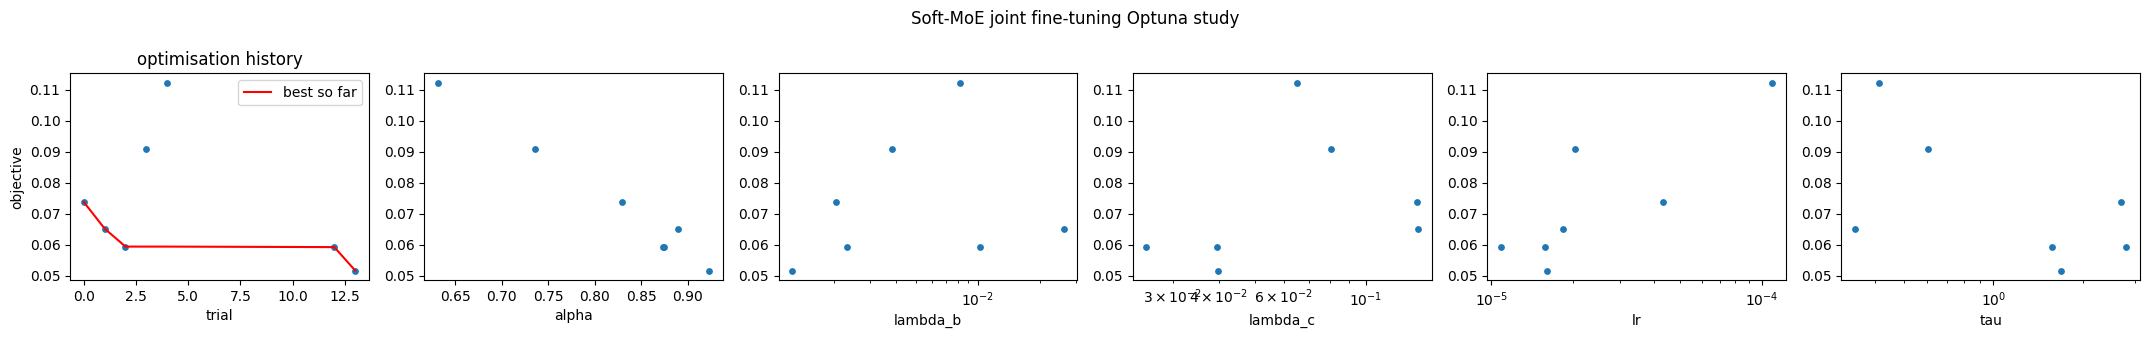
\includegraphics[width=\textwidth]{t3_optuna.png}}\\
\subfloat[Joint fine-tuning curves.\label{fig:t3curves}]{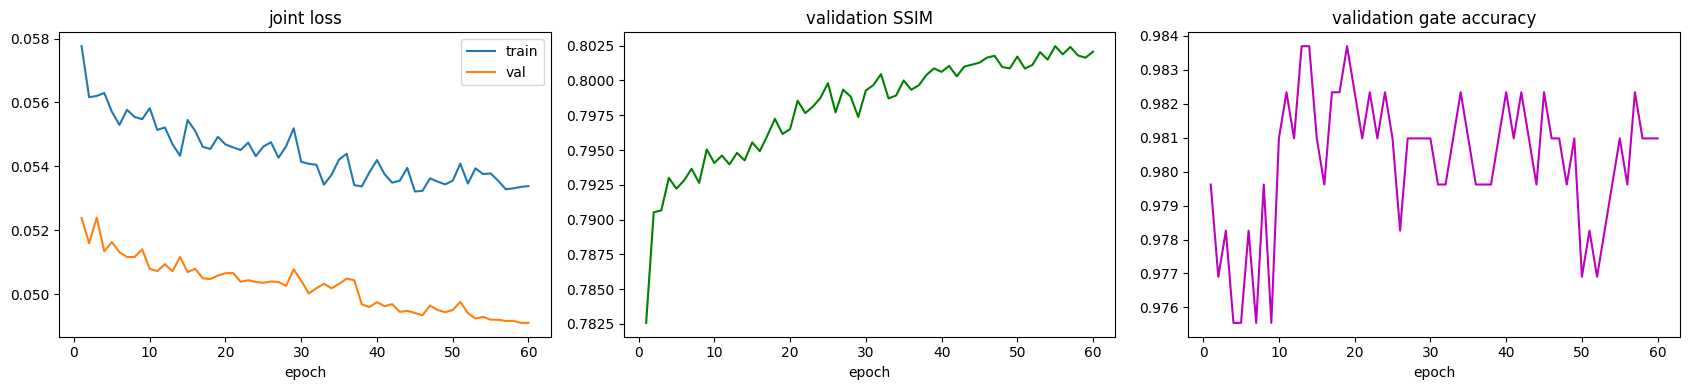
\includegraphics[width=0.9\textwidth]{t3_training_curves.png}}
\caption{Task 3 hyperparameter search and joint training.}
\end{figure*}

\subsection{Reconstruction results}
Table~\ref{tab:t3res} compares all restoration systems on the identical test manifest. The soft MoE beats hard routing (oracle and predicted) on \emph{every} corrupted type and severity. The gains are largest where the corruption is mild or ambiguous: low occlusion $+0.106$ SSIM over predicted routing, low blur $+0.072$ and medium occlusion $+0.072$. On high salt-and-pepper, where one expert is already near-certain, the gain is small ($+0.002$). Clean inputs stay almost untouched (SSIM 0.997) because the identity branch carries 95\% of the weight. Pooled over the test manifest the soft MoE reaches L1 0.0392, SSIM 0.764 and PSNR 27.50\,dB. Fig.~\ref{fig:t3hvs} shows the qualitative difference: the soft output blends in part of the input, which keeps fine detail and colour that the hard-routed expert smooths away.

\begin{table}[!t]
\caption{Test SSIM / PSNR (dB) of all restoration systems}
\label{tab:t3res}
\centering\footnotesize
\setlength{\tabcolsep}{2.5pt}
\resizebox{\columnwidth}{!}{%
\begin{tabular}{@{}llcccccc@{}}
\toprule
 & & \multicolumn{4}{c}{SSIM$\uparrow$} & \multicolumn{2}{c}{PSNR$\uparrow$}\\
\cmidrule(lr){3-6}\cmidrule(l){7-8}
Type & Sev. & T1 & T2-or. & T2-pr. & \textbf{T3} & T2-pr. & \textbf{T3}\\
\midrule
Clean & -- & 0.406 & 1.000 & 0.998 & 0.997 & 79.4$^\ast$ & 57.3\\
\multirow{3}{*}{S\&P} & low & 0.406 & 0.706 & 0.706 & \textbf{0.745} & 24.24 & \textbf{25.16}\\
 & med. & 0.406 & 0.703 & 0.703 & \textbf{0.715} & 24.20 & \textbf{24.57}\\
 & high & 0.405 & 0.695 & 0.695 & \textbf{0.697} & 24.05 & \textbf{24.31}\\
\multirow{3}{*}{Blur} & low & 0.406 & 0.721 & 0.755 & \textbf{0.827} & 25.34 & \textbf{26.73}\\
 & med. & 0.406 & 0.716 & 0.716 & \textbf{0.756} & 24.43 & \textbf{25.40}\\
 & high & 0.405 & 0.695 & 0.695 & \textbf{0.716} & 24.09 & \textbf{24.71}\\
\multirow{3}{*}{Occl.} & low & 0.392 & 0.688 & 0.696 & \textbf{0.803} & 22.62 & \textbf{24.23}\\
 & med. & 0.377 & 0.654 & 0.655 & \textbf{0.726} & 21.47 & \textbf{22.28}\\
 & high & 0.357 & 0.607 & 0.607 & \textbf{0.656} & 19.94 & \textbf{20.36}\\
\bottomrule
\multicolumn{8}{@{}l}{\scriptsize T1: Task 1 (evaluated checkpoint); T2-or./pr.: oracle/predicted hard routing; T3: soft MoE.}
\end{tabular}}
\end{table}

\begin{figure}[!t]
\centering
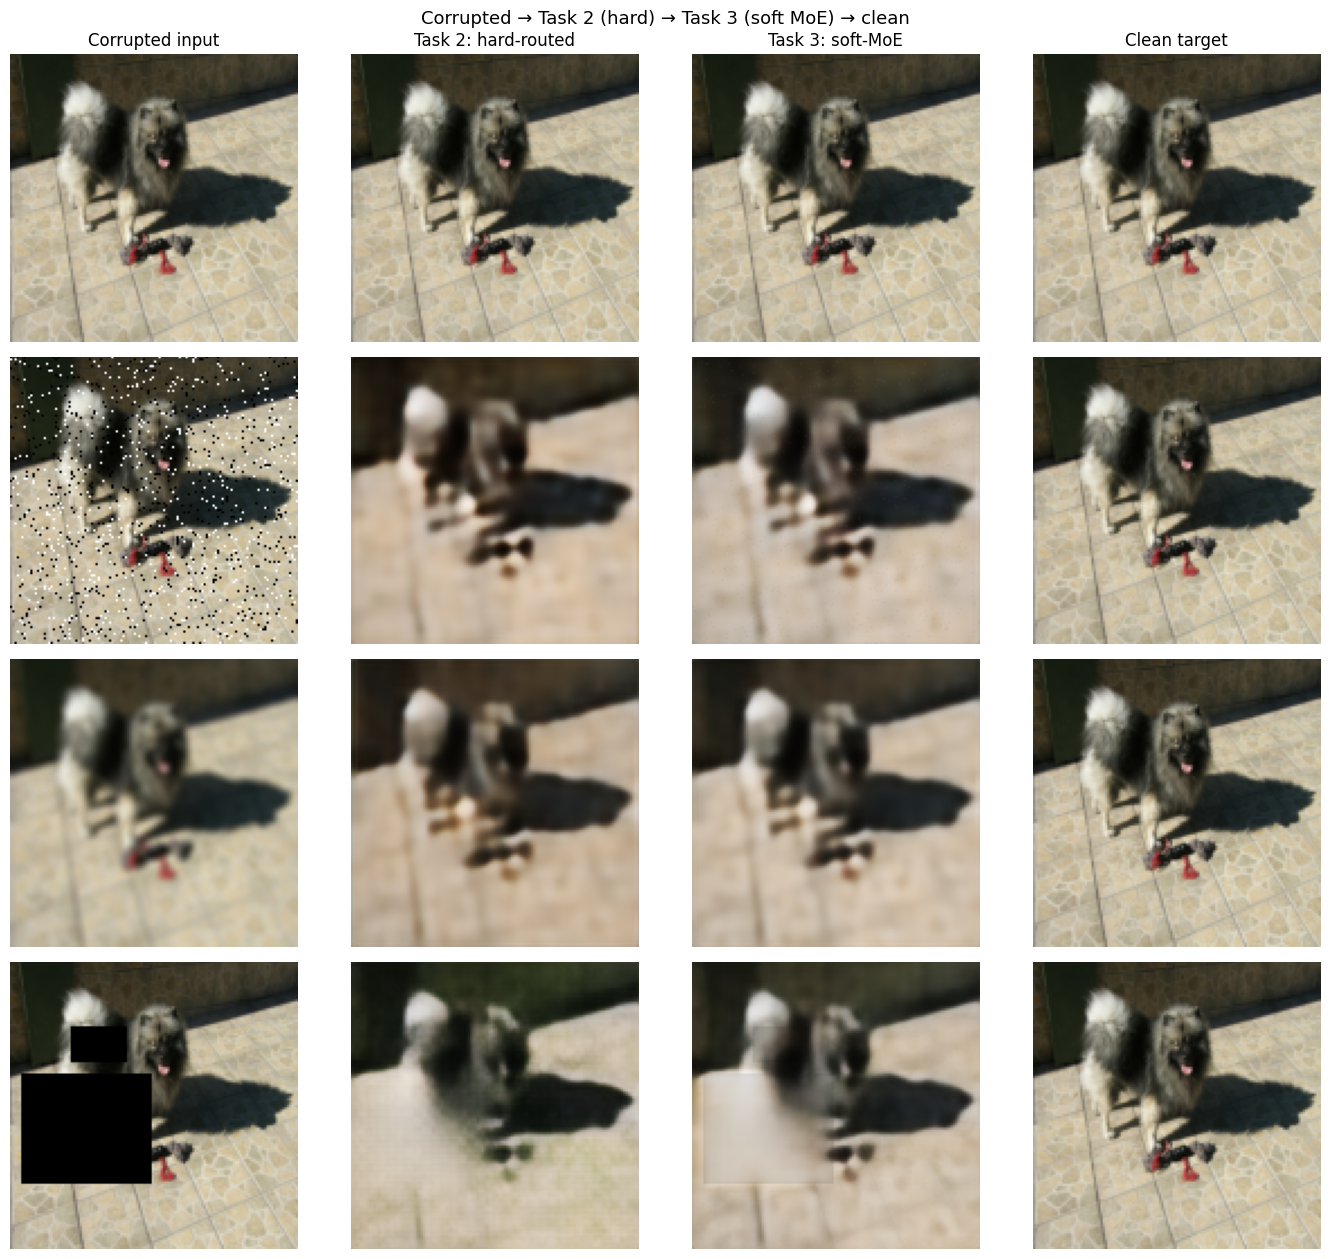
\includegraphics[width=\columnwidth]{t3_hard_vs_soft.png}
\caption{Corrupted input, Task 2 hard routing, Task 3 soft MoE and clean target (clean, salt-and-pepper, blur and occlusion inputs).}
\label{fig:t3hvs}
\end{figure}

\subsection{Gating behaviour}
Table~\ref{tab:t3w} gives the mean weights for every true type and severity, and Fig.~\ref{fig:t3heat} the routing heatmap. Every row peaks on its matching branch: clean 0.954, salt-and-pepper 0.931, blur 0.755 and occlusion 0.804. Routing becomes sharper as severity increases (own-expert weight on blur: 0.68, 0.79, 0.79; on occlusion: 0.72, 0.83, 0.87), while mild corruptions keep a substantial identity weight (0.32 on low blur, 0.26 on low occlusion). This smooth, severity-dependent hedging is exactly what hard routing cannot express, and it explains the gains in Table~\ref{tab:t3res}. In the low-entropy examples (Fig.~\ref{fig:t3dom}a) a single branch takes $>0.99$ of the weight. In the high-entropy examples (Fig.~\ref{fig:t3dom}b) mild blur and occlusion inputs split weight between the identity, blur and occlusion branches (e.g.\ 0.41/0.31/0.28).

\emph{Inactive or dominating experts.} The dataset-wide mean weights are 0.243 (identity), 0.281 (salt-and-pepper), 0.233 (blur) and 0.243 (occlusion), all close to $\tfrac14$, so no expert is inactive. No expert dominates unrelated inputs: the salt-and-pepper expert receives at most 0.010 on any other type, the blur expert at most 0.035 (on clean images) and the occlusion expert at most 0.009. The only notable cross-talk is the identity branch on mild blur and occlusion, which is intended behaviour.

\begin{table}[!t]
\caption{Mean routing weights by true corruption type and severity (test)}
\label{tab:t3w}
\centering\footnotesize
\begin{tabular}{@{}llcccc@{}}
\toprule
Type & Sev. & $w_0$ (id.) & $w_1$ (S\&P) & $w_2$ (blur) & $w_3$ (occl.)\\
\midrule
Clean & -- & \textbf{0.954} & 0.001 & 0.035 & 0.009\\
\multirow{3}{*}{S\&P} & low & 0.117 & \textbf{0.880} & 0.000 & 0.003\\
 & med. & 0.045 & \textbf{0.954} & 0.000 & 0.001\\
 & high & 0.040 & \textbf{0.958} & 0.000 & 0.001\\
\multirow{3}{*}{Blur} & low & 0.317 & 0.000 & \textbf{0.681} & 0.002\\
 & med. & 0.211 & 0.000 & \textbf{0.788} & 0.001\\
 & high & 0.205 & 0.000 & \textbf{0.794} & 0.001\\
\multirow{3}{*}{Occl.} & low & 0.261 & 0.010 & 0.014 & \textbf{0.716}\\
 & med. & 0.160 & 0.005 & 0.008 & \textbf{0.826}\\
 & high & 0.120 & 0.003 & 0.006 & \textbf{0.871}\\
\bottomrule
\end{tabular}
\end{table}

\begin{figure}[!t]
\centering
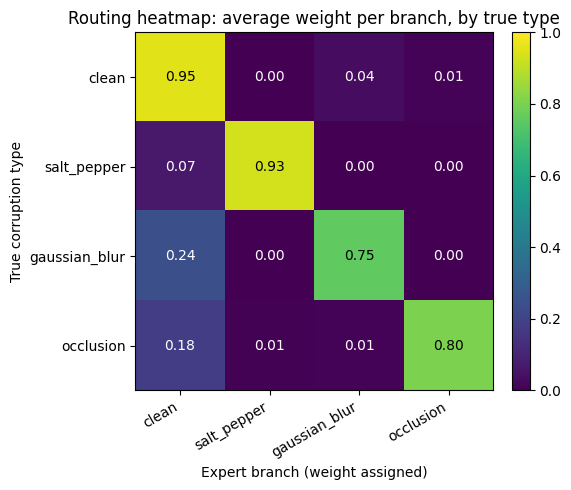
\includegraphics[width=0.8\columnwidth]{t3_routing_heatmap.png}
\caption{Routing heatmap: mean branch weight per true corruption type.}
\label{fig:t3heat}
\end{figure}

\begin{figure*}[!t]
\centering
\subfloat[One expert dominates (lowest routing entropy).]{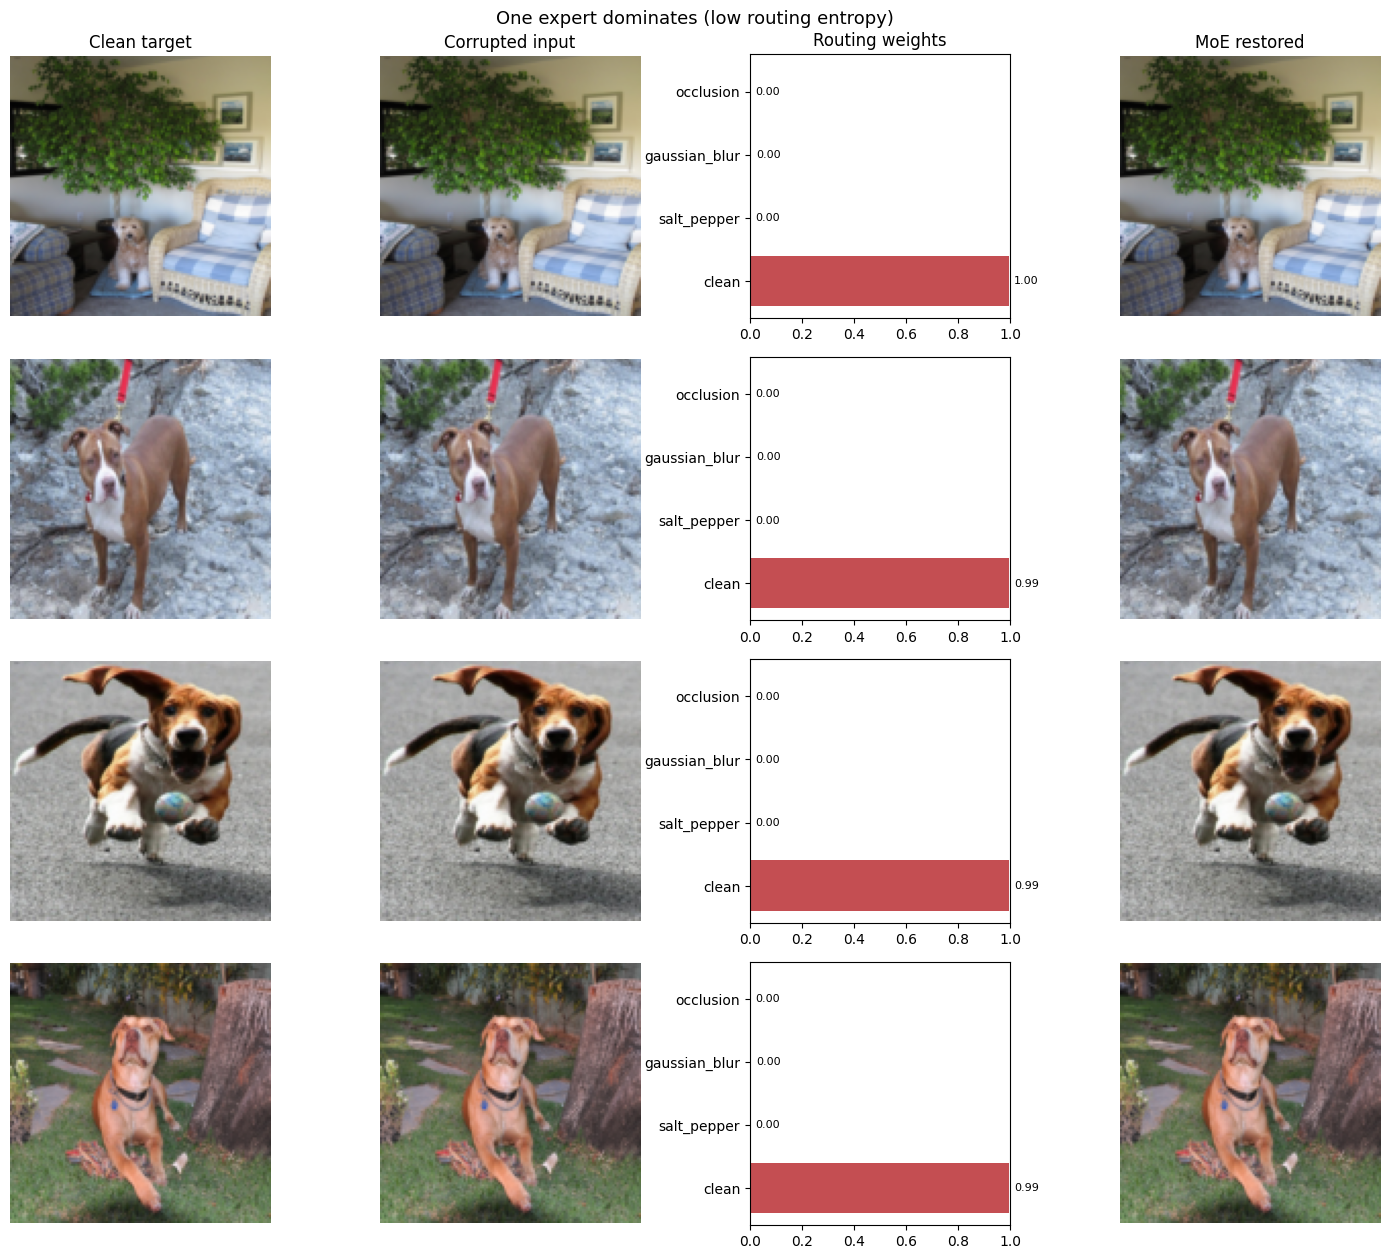
\includegraphics[width=0.49\textwidth]{t3_dominant.png}}\hfill
\subfloat[Weights spread across experts (highest routing entropy).]{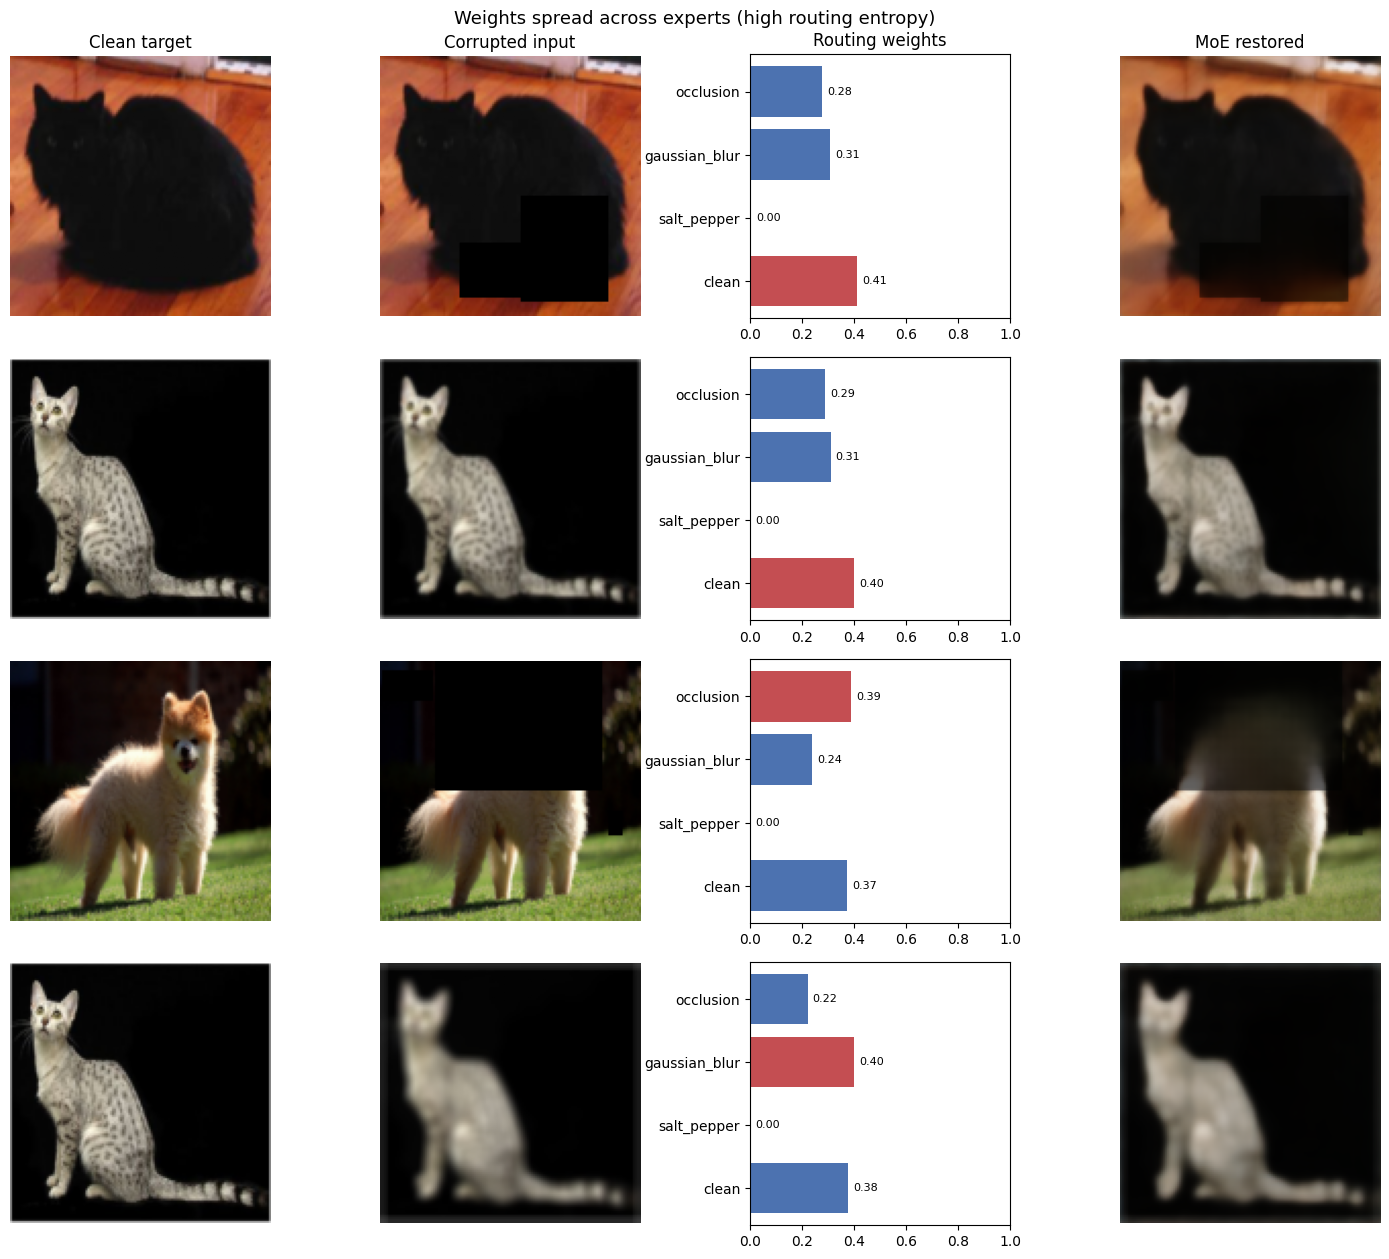
\includegraphics[width=0.49\textwidth]{t3_distributed.png}}
\caption{Soft-MoE routing examples: clean target, corrupted input, routing weights (red: strongest branch) and output.}
\label{fig:t3dom}
\end{figure*}

\subsection{Failure cases and limitations}
Fig.~\ref{fig:t3fail} shows the lowest-SSIM output for each corruption: high salt-and-pepper (0.381) and high blur (0.339) on a heavily textured field of flowers, and high occlusion (0.373), where most of a dog is masked. The occlusion output shows the main limitation of pixel-space mixing. With 0.12 identity weight, a faint trace of the black rectangles remains, and the expert's fill is a smooth, low-detail patch. Further limitations:
\begin{itemize}
\item All three experts run on every input, about $3\times$ the compute of hard routing.
\item The balance target assumes a balanced corruption prior.
\item The gate was trained on single corruptions only, so behaviour on genuinely mixed corruptions is extrapolation.
\end{itemize}
The single-graph ONNX export (gate, three experts and weighted sum) reproduces PyTorch to $4.8{\times}10^{-7}$ (image) and $2.4{\times}10^{-7}$ (weights).

\begin{figure}[!t]
\centering
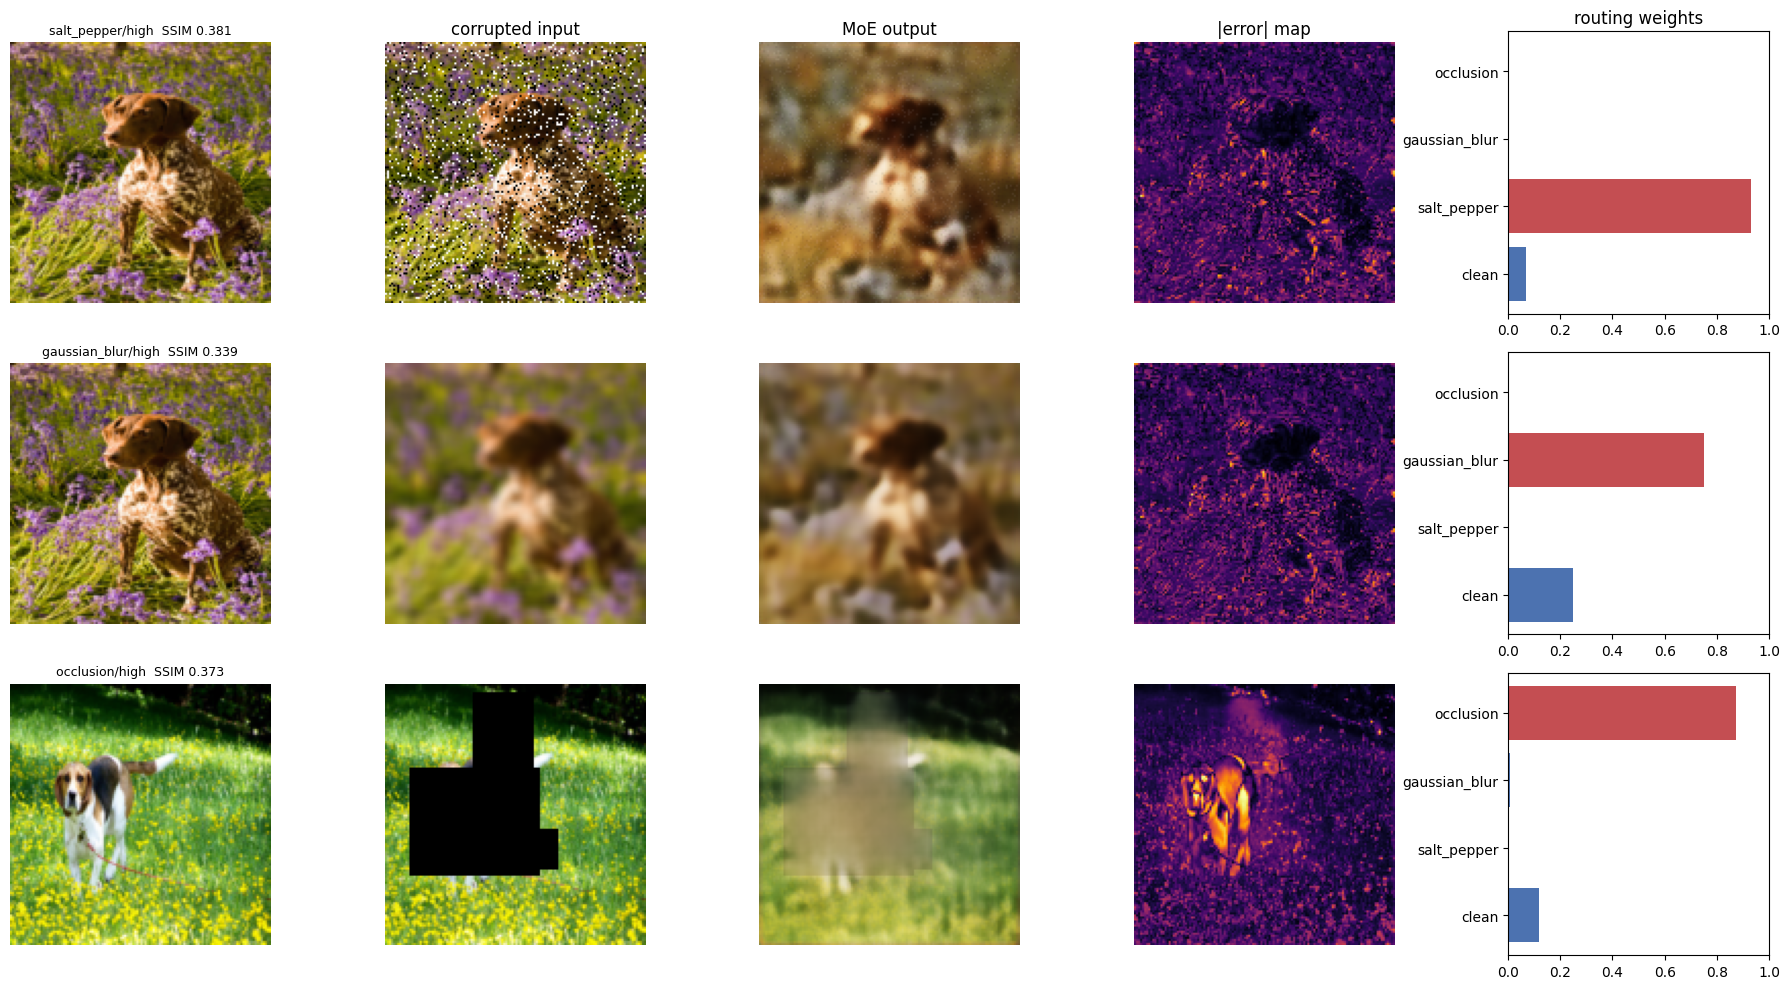
\includegraphics[width=\columnwidth]{t3_failures.png}
\caption{Task 3 failure cases (lowest SSIM per corruption) with error maps and routing weights.}
\label{fig:t3fail}
\end{figure}

%=====================================================================
\section{Task 4: Style-Conditioned Face-to-Sketch cGAN}\label{sec:t4}
\subsection{Architecture and losses}
The generator $\hat y=G(x,s)$ is a five-level U-Net (Fig.~\ref{fig:t4arch}).
\begin{itemize}
\item The style $s\in\{0,1,2\}$ is mapped by a learned embedding (dimension 16). The embedding is concatenated with the photo at the input and with the bottleneck features, and it is re-injected by FiLM in \emph{every} decoder block.
\item Upsampling uses resize-convolution, and dropout is used in the deepest decoder blocks.
\item The output layer is a tanh.
\end{itemize}
The PatchGAN discriminator $D(x,y,s)$ receives the photo, a real or generated sketch and the broadcast style embedding (its own learned embedding), and outputs a $14{\times}14$ map of patch logits. Losses use BCE with logits:
\begin{equation}
\mathcal{L}_D=\tfrac12\bigl[\mathrm{BCE}(D(x,y,s),1)+\mathrm{BCE}(D(x,G(x,s),s),0)\bigr],
\end{equation}
\begin{equation}
\mathcal{L}_G=\mathrm{BCE}(D(x,G(x,s),s),1)+\lambda_{L1}\lVert y-G(x,s)\rVert_1.
\end{equation}
With the selected configuration, $G$ has 7.12\,M parameters and $D$ 1.57\,M. The style conditioning is effective: the same photo produces clearly different sketches for different styles (Fig.~\ref{fig:t4gal}).

\begin{figure}[!t]
\centering
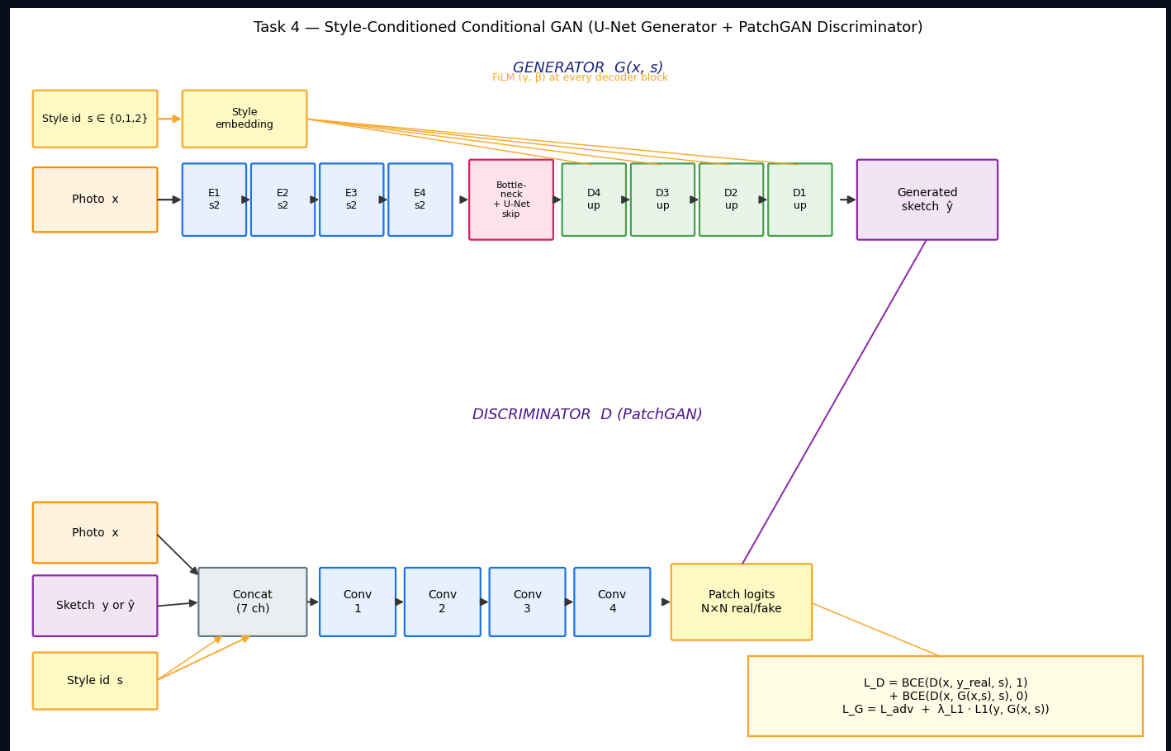
\includegraphics[width=\columnwidth]{t4_arch.png}
\caption{Task 4: style-conditioned U-Net generator (FiLM at every decoder block) and style-conditioned PatchGAN discriminator.}
\label{fig:t4arch}
\end{figure}

\begin{figure}[!t]
\centering
\subfloat[Training pairs, two per style.]{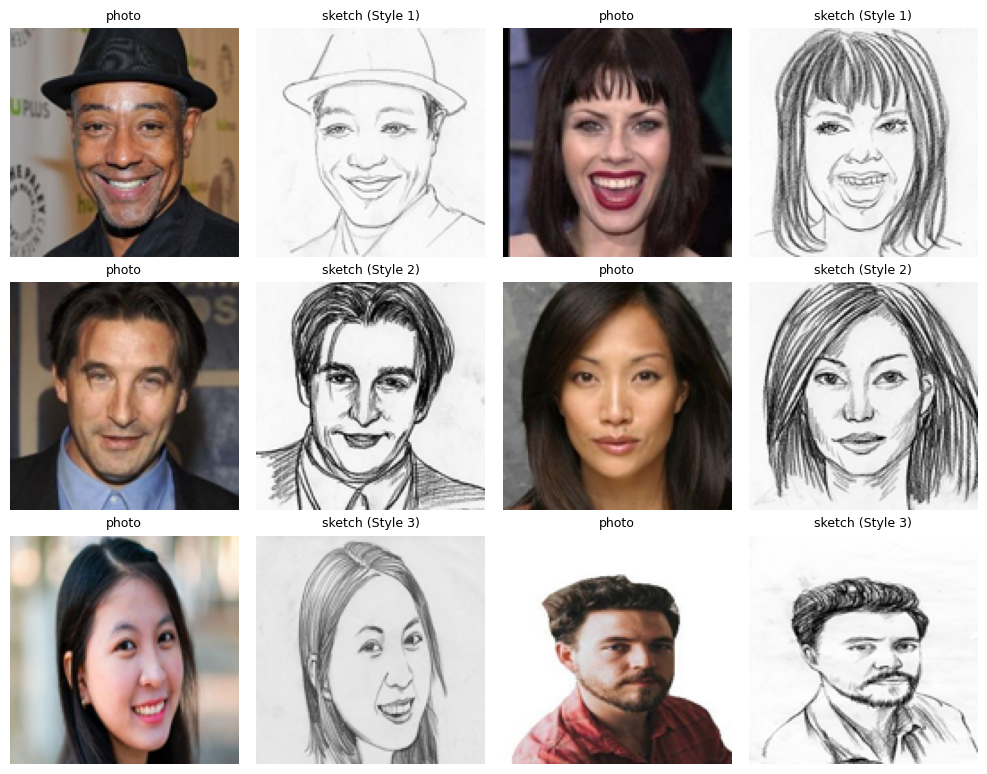
\includegraphics[width=0.49\columnwidth]{t4_pairs.png}}\hfill
\subfloat[Identical paired augmentation.]{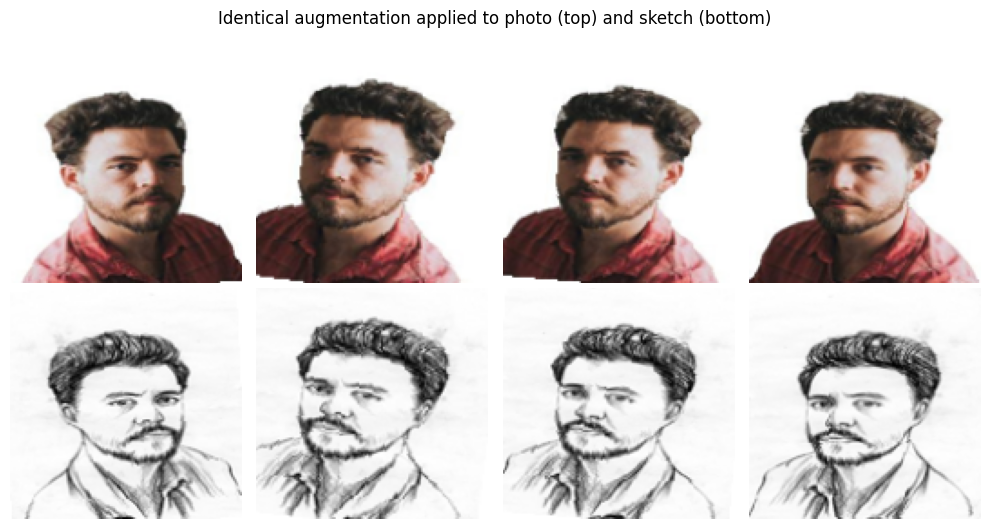
\includegraphics[width=0.49\columnwidth]{t4_paired_augmentation.png}}
\caption{FS2K data at $128{\times}128$: photo--sketch pairs and identical spatial augmentation of both members of a pair.}
\label{fig:t4data}
\end{figure}

\subsection{Hyperparameter search and training}
The Optuna search (Fig.~\ref{fig:t4optuna}) tuned the generator and discriminator learning rates, batch size, base channels, dropout, style-embedding dimension and $\lambda_{L1}\in[20,200]$ around the pix2pix default of 100. It ran 15 shortened trials of 5 epochs, objective validation L1, with pruning on the median rule, mode collapse (output-diversity ratio $<0.15$) and an overpowering discriminator ($>$99\% real and fake accuracy). Ten trials completed and five were pruned. Selected: $G$ learning rate $4.54{\times}10^{-4}$, $D$ learning rate $6.83{\times}10^{-5}$, batch 8, base 48, dropout 0.195, embedding 16 and $\lambda_{L1}{=}137.3$.

The selected configuration was then retrained on the full schedule: 10 epochs of L1-only generator pre-training (a pix2pix stabilisation trick), then adversarial training with Adam ($\beta_1{=}0.5$) for up to 150 epochs, with early stopping (patience 25) on validation L1. Training was resumed across Colab sessions and stopped at epoch 59, with the best validation L1 of 0.1895 (in $[-1,1]$ units). Fig.~\ref{fig:t4curves} records the discriminator real and fake losses, the generator adversarial and reconstruction losses and the validation measurements \emph{separately}. The discriminator stays in a healthy band (real/fake accuracy $\approx$0.76/0.82, losses $\approx$0.47/0.42) without overpowering the generator. Training L1 keeps decreasing while validation L1 plateaus at $\approx$0.19, which is the reason for early stopping. Fig.~\ref{fig:t4fixed} shows the same six validation photos logged at fixed intervals: blurry, low-contrast strokes at epoch 1 become clean, style-specific line work later.

\begin{figure*}[!t]
\centering
\subfloat[Optuna study (15 trials; 5 pruned).\label{fig:t4optuna}]{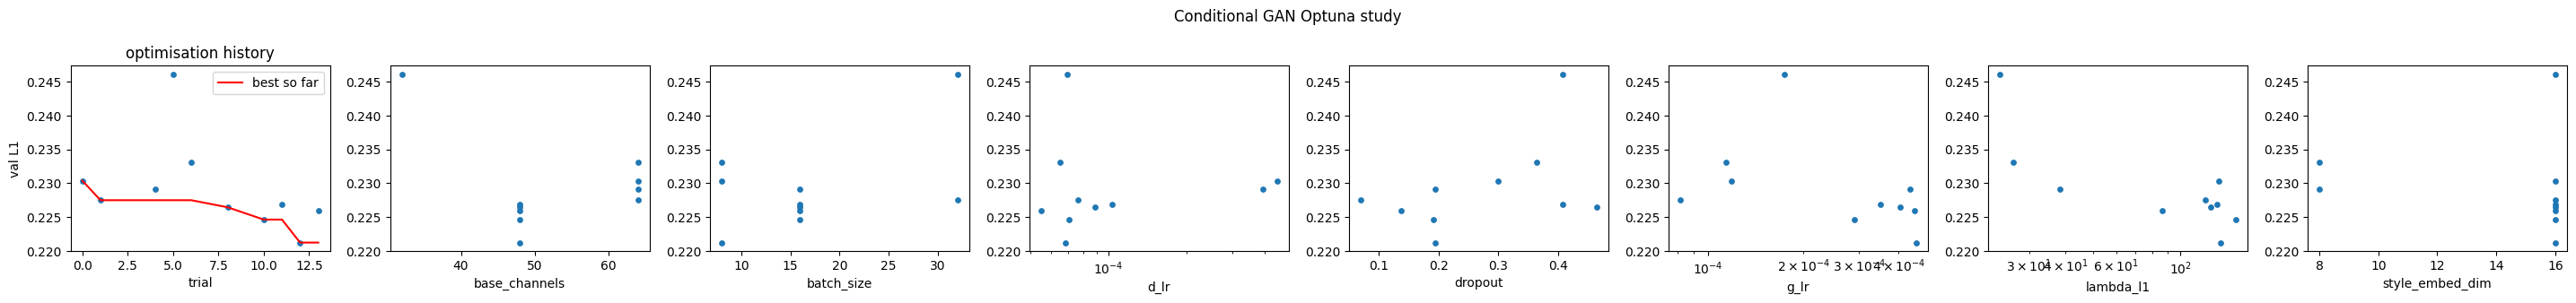
\includegraphics[width=\textwidth]{t4_optuna.png}}\\
\subfloat[Separately recorded losses and discriminator accuracies.\label{fig:t4curves}]{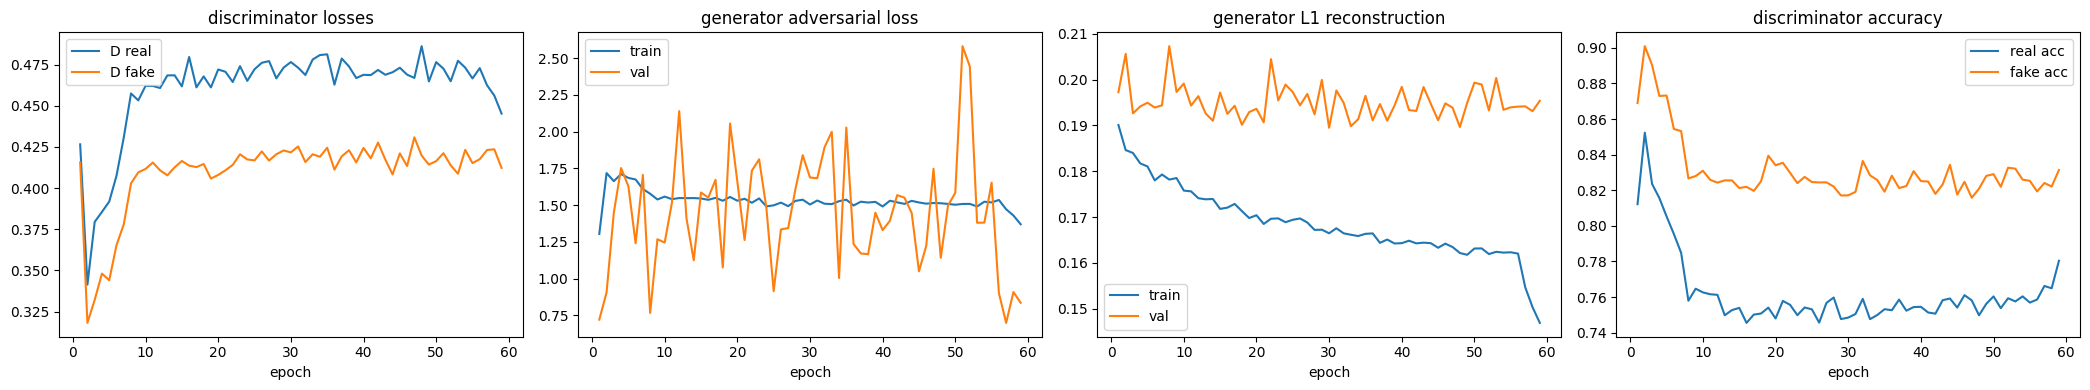
\includegraphics[width=\textwidth]{t4_training_curves.png}}
\caption{Task 4 hyperparameter search and adversarial training.}
\end{figure*}

\begin{figure}[!t]
\centering
\subfloat[Epoch 1.]{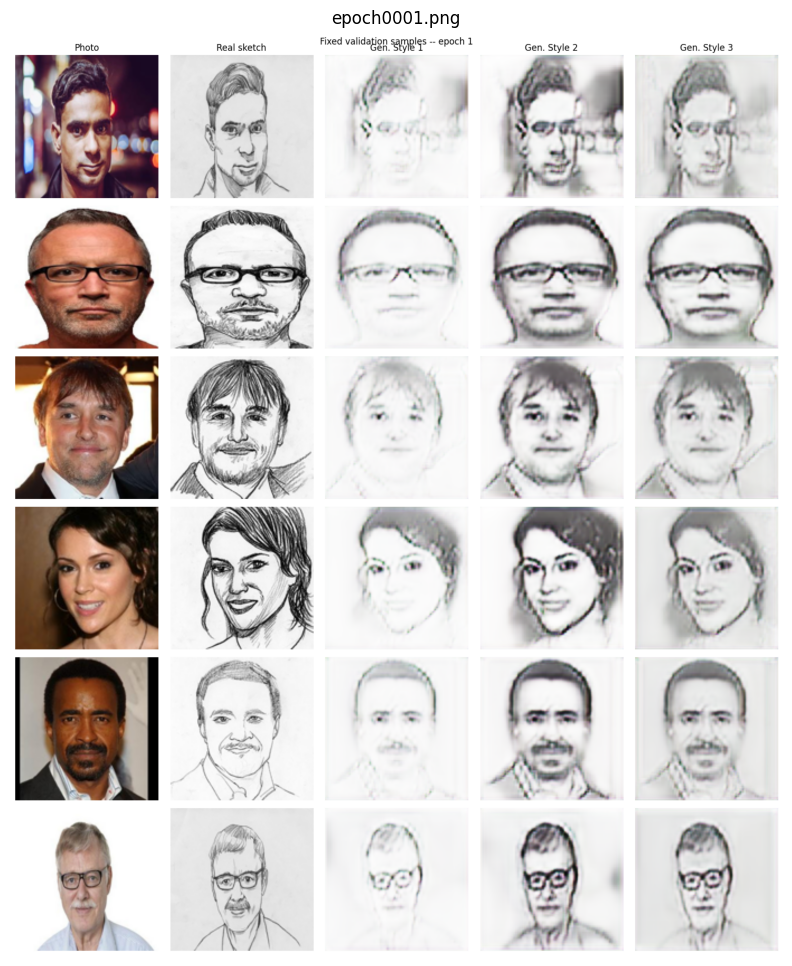
\includegraphics[width=0.49\columnwidth]{t4_fixed_epoch001.png}}\hfill
\subfloat[Epoch 65 (last logged grid).]{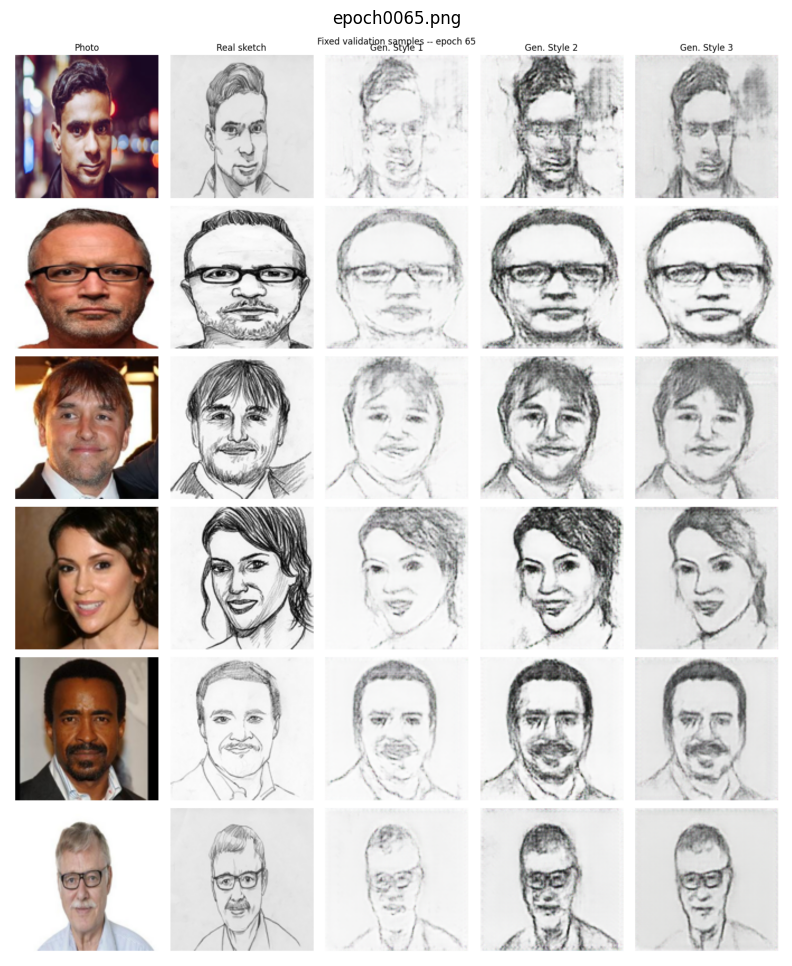
\includegraphics[width=0.49\columnwidth]{t4_fixed_epoch065.png}}
\caption{Fixed validation photos rendered in all three styles during training (photo, real sketch, generated Styles 1--3).}
\label{fig:t4fixed}
\end{figure}

\subsection{Results}
Table~\ref{tab:t4res} reports the official test set results, generated with each pair's true style. Style~3 is reproduced best (SSIM 0.620, PSNR 18.9\,dB). Style~2's dense, high-contrast cross-hatching is hardest for a pixel metric (SSIM 0.391), since small stroke misalignments are penalised twice. To measure style controllability, each test photo is rendered in all three styles and we record which output is closest (L1) to the ground truth (Fig.~\ref{fig:t4conf}). The true style wins for 97\% of Style~2 and 98\% of Style~3 photos, and for 73\% of Style~1 photos; the rest are closest to Style~3, its most similar light pencil style. Weighted over the test set, the true style wins for $\approx$83\% of photos. The mode-collapse diversity ratios on 16 test photos are 0.46, 0.82 and 0.56 (collapse threshold 0.25), so the generator follows its input in all styles. Fig.~\ref{fig:t4gal} shows two test photos of every ground-truth style rendered in all three styles. The ONNX generator matches PyTorch to $\le 4.0{\times}10^{-6}$ for all styles.

\begin{table}[!t]
\caption{Task 4 results on the official FS2K test set (1{,}046 pairs)}
\label{tab:t4res}
\centering\footnotesize
\begin{tabular}{@{}lcccc@{}}
\toprule
Style (test pairs) & L1$^\dagger\downarrow$ & SSIM$\uparrow$ & PSNR (dB)$\uparrow$\\
\midrule
Style 1 (619) & 0.204 & 0.464 & 15.93\\
Style 2 (381) & 0.316 & 0.391 & 12.14\\
Style 3 (46) & 0.127 & 0.620 & 18.87\\
\midrule
Overall & 0.241 & 0.444 & 14.68\\
\bottomrule
\multicolumn{4}{@{}l}{\scriptsize $^\dagger$L1 in $[-1,1]$ units; SSIM and PSNR on $[0,1]$ images.}
\end{tabular}
\end{table}

\begin{figure}[!t]
\centering
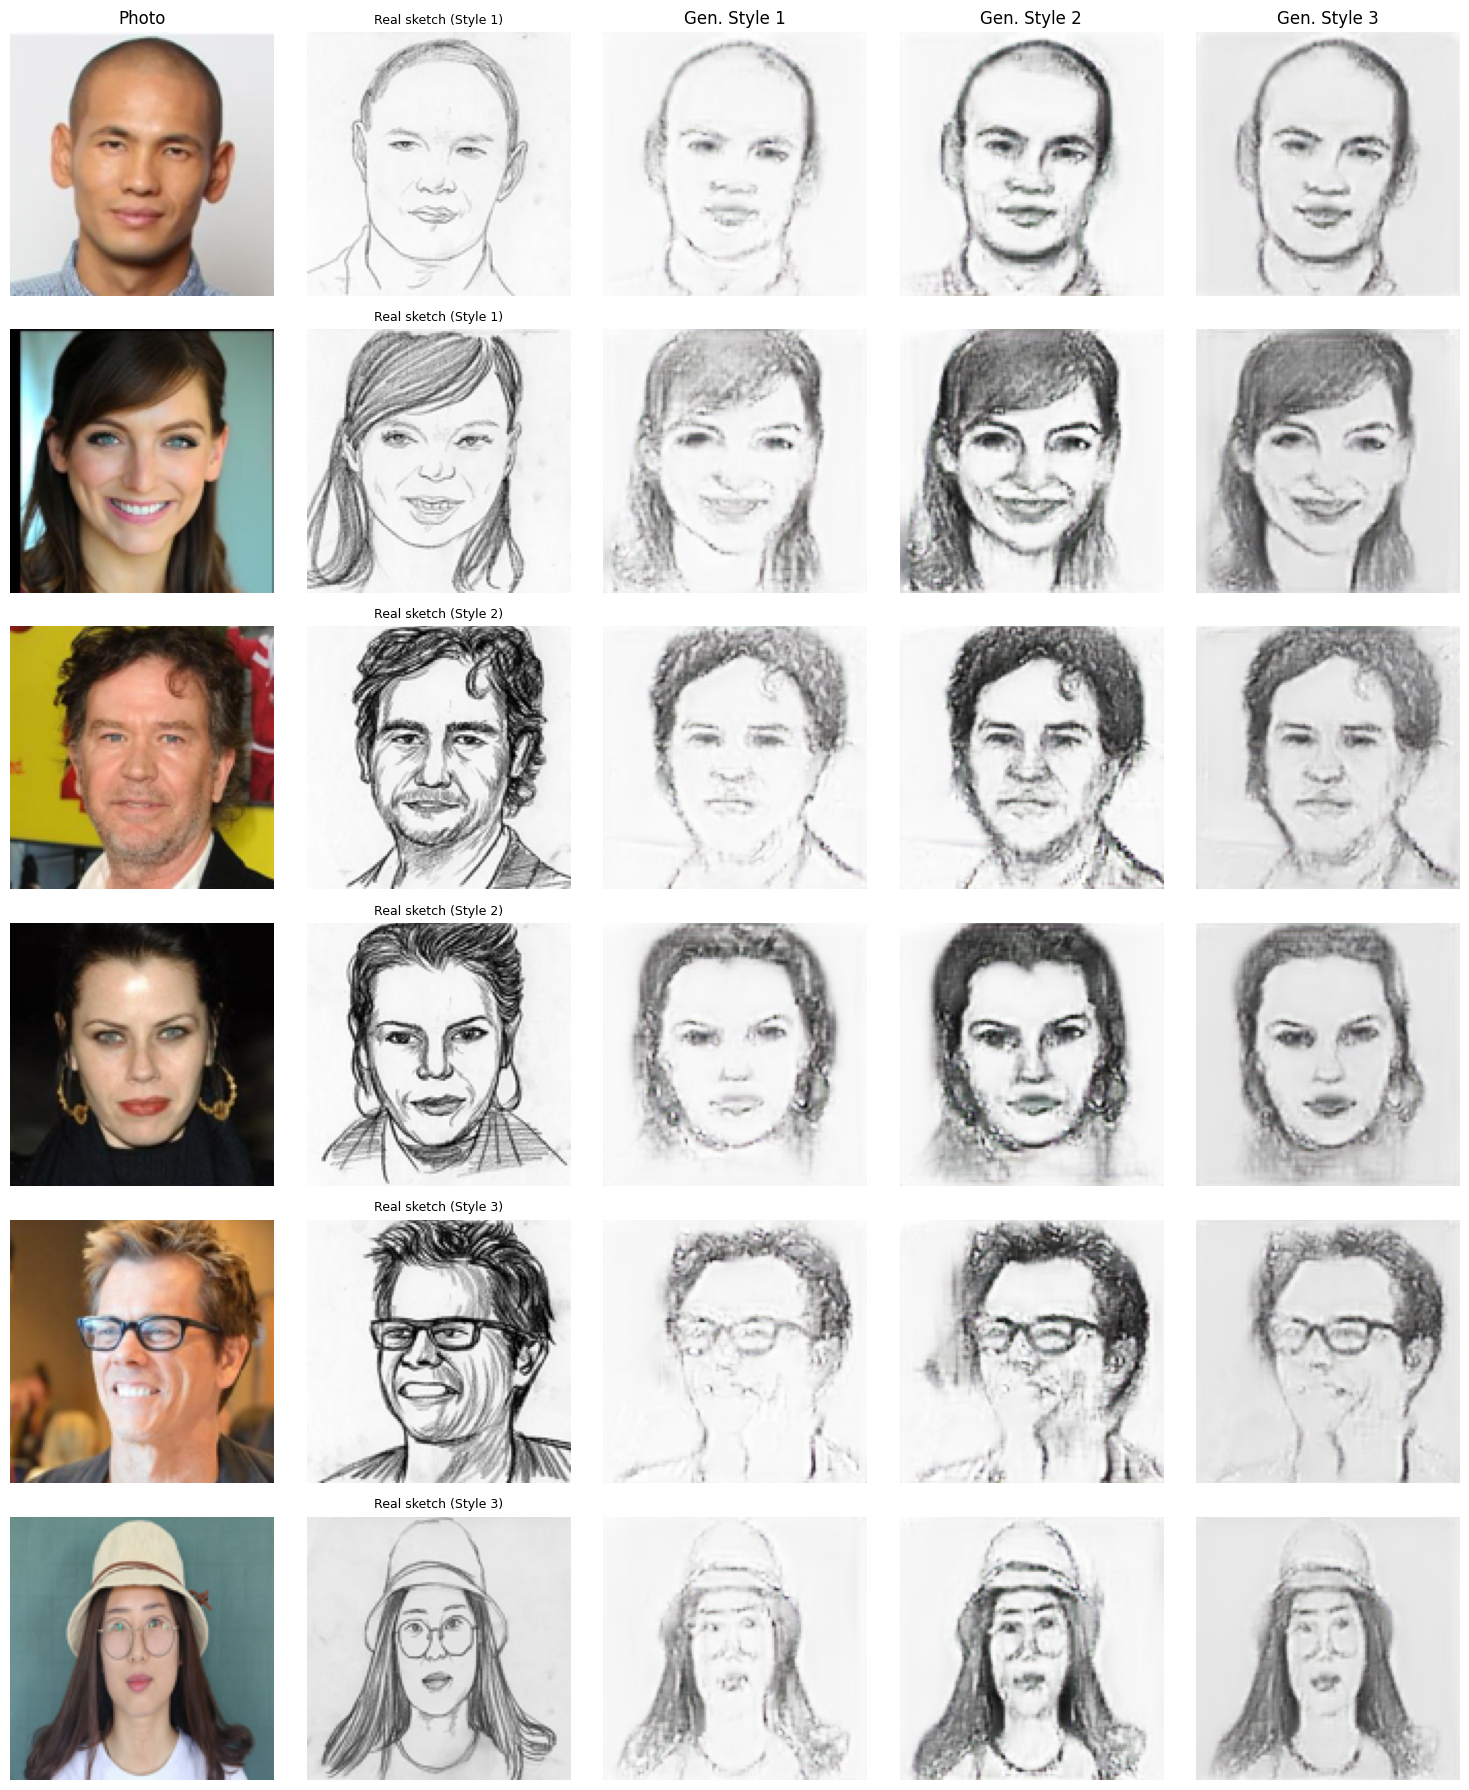
\includegraphics[width=\columnwidth]{t4_test_gallery.png}
\caption{Official test photos (two per ground-truth style): photo, real sketch and generated Styles 1--3.}
\label{fig:t4gal}
\end{figure}

\begin{figure}[!t]
\centering
\subfloat[Failure cases with error maps.\label{fig:t4fail}]{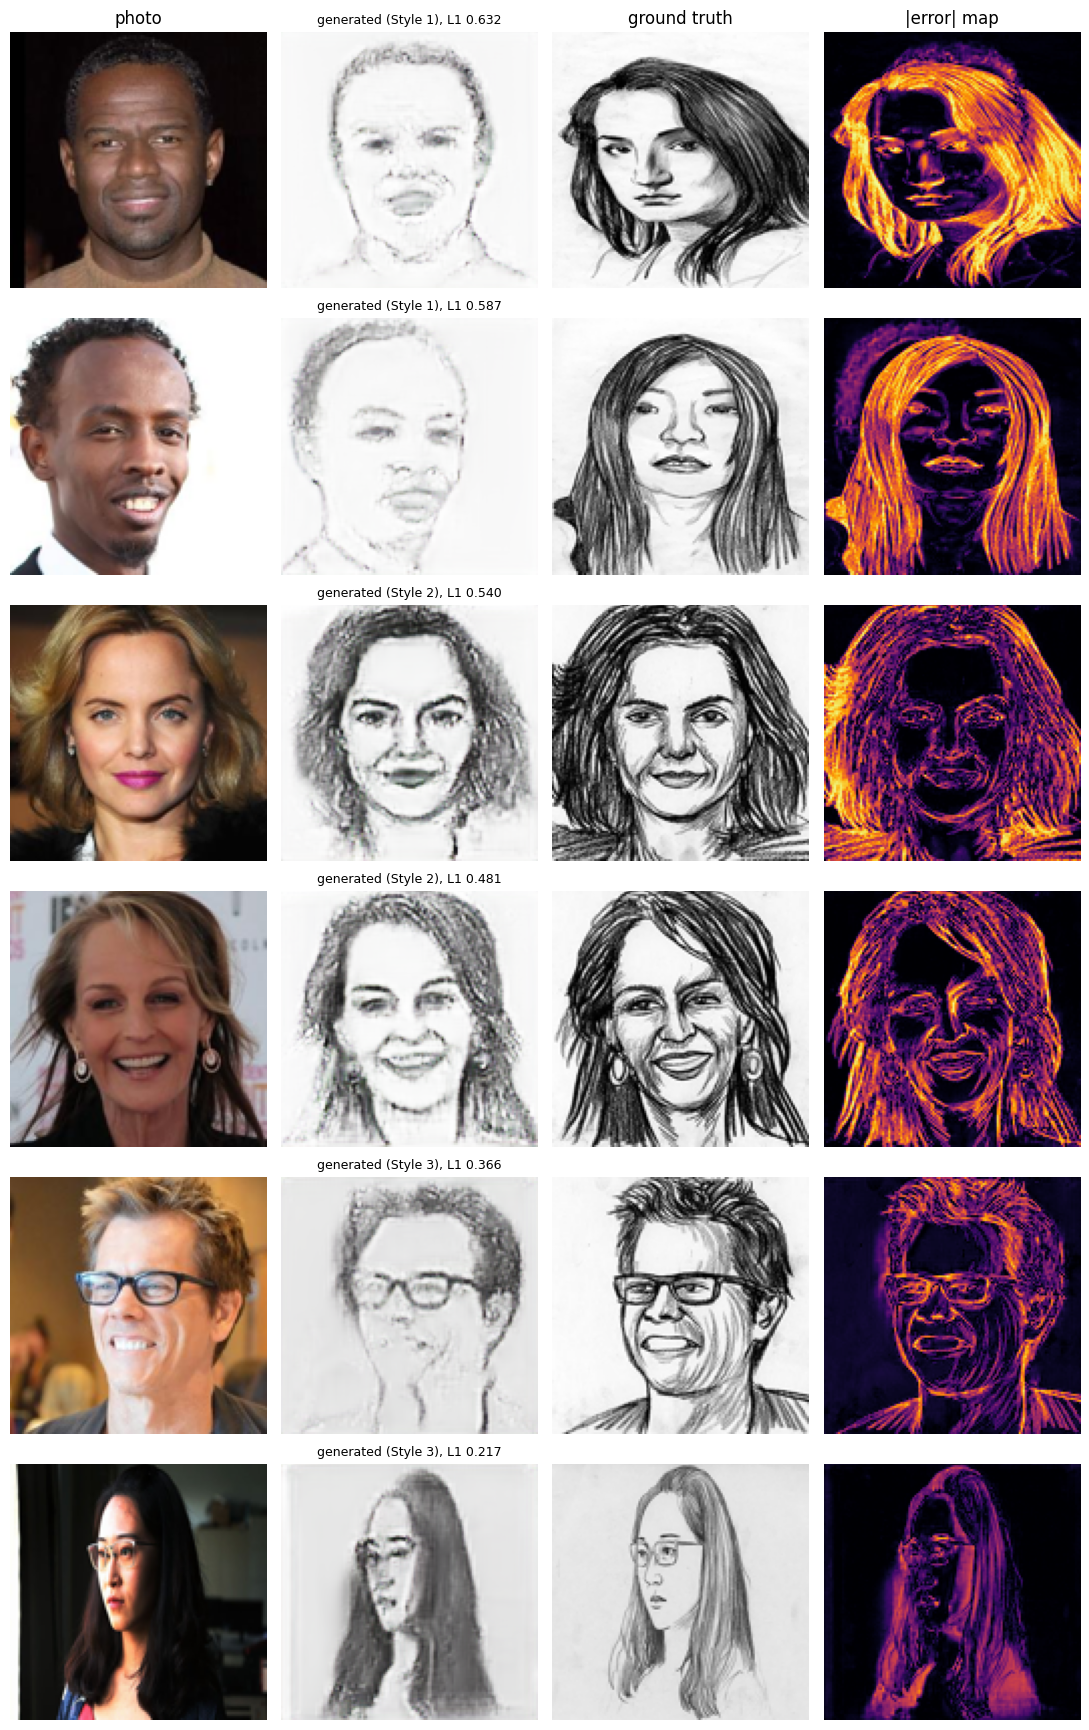
\includegraphics[width=0.56\columnwidth]{t4_failures.png}}\hfill
\subfloat[Style confusion.\label{fig:t4conf}]{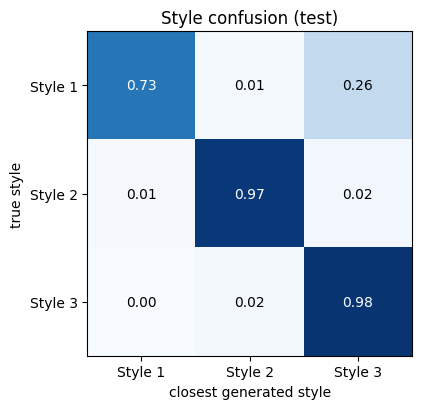
\includegraphics[width=0.42\columnwidth]{t4_style_confusion.png}}
\caption{Task 4 failure analysis: (a) the two highest-L1 test outputs per style; (b) which generated style is closest to the ground truth.}
\end{figure}

\subsection{Failure analysis}
Three failure types appear.
\begin{itemize}
\item \emph{Artifacts.} Hair is the dominant error region in every style (Fig.~\ref{fig:t4fail}), because artists draw strands freely and the L1 term averages them into soft grey texture. Faint checkerboard texture remains in dark clothing.
\item \emph{Style confusion.} Style~1 sometimes collapses towards the heavier Style~3 rendering (26\%).
\item \emph{Pairing errors.} The two worst Style~1 cases pair a man's photo with a woman's sketch. The file resolver falls back to matching sketches by base filename when the per-folder path does not match. FS2K restarts numbering in each of its three sub-folders, so some photos are paired with a sketch from another folder.
\end{itemize}
These mismatched pairs inflate the measured Style~1 error and add noise to training. Matching sketches by \emph{folder index plus id} fixes the problem, and this is the first item of future work. No mode collapse was observed.

%=====================================================================
\section{ONNX Export, Application and Deployment}\label{sec:app}
\subsection{ONNX export and verification}
The following models are exported with opset 17 and dynamic batch size:
\begin{itemize}
\item the Task 1 universal autoencoder;
\item the Task 2 classifier and three specialists;
\item the complete Task 3 soft-MoE pipeline as a single graph with two outputs (restored image and routing weights);
\item the Task 4 generator, with inputs photo and \texttt{style\_idx}. The discriminator is training-only and is not exported.
\end{itemize}
Each export is checked with \texttt{onnx.checker} and compared with PyTorch on real test inputs (Table~\ref{tab:onnx}).

\begin{table}[!t]
\caption{ONNX Runtime vs PyTorch (real test inputs)}
\label{tab:onnx}
\centering\footnotesize
\begin{tabular}{@{}lcc@{}}
\toprule
Model & Max $|\Delta|$ & Mean $|\Delta|$\\
\midrule
Task 1 universal AE & $4.5{\times}10^{-6}$ & $1.6{\times}10^{-7}$\\
Task 2 classifier (logits) & $8.1{\times}10^{-6}$ & argmax 100\%\\
Task 2 salt-and-pepper / blur / occl. & $2.6/2.1/2.1{\times}10^{-5}$ & $\le3.0{\times}10^{-7}$\\
Task 3 soft MoE (image / weights) & $4.8/2.4{\times}10^{-7}$ & --\\
Task 4 generator (3 styles) & $\le4.0{\times}10^{-6}$ & $\le1.7{\times}10^{-7}$\\
\bottomrule
\end{tabular}
\end{table}

\subsection{Interface design and implementation}
The interface was first designed in Google Stitch. Fig.~\ref{fig:stitch} shows the original Stitch canvas: the prompt history and the generated \emph{Universal Restoration} screen with the four workspace tabs, degradation and severity controls, side-by-side input and reconstruction panels, and verdict and timing cards. The telemetry values in this mock-up are Stitch's placeholders, not measurements. The implementation follows its layout, card structure and controls in a single React application styled with Tailwind CSS. It has four tabs, one per workspace (Fig.~\ref{fig:app}):
\begin{itemize}
\item \emph{Universal Restoration}: upload, corruption type and severity, input/corrupted/restored panels, the selected settings, inference time and download.
\item \emph{Hard-Routed Restoration}: the four class probabilities, predicted corruption, selected expert, output and time.
\item \emph{Soft Mixture-of-Experts Restoration}: all four routing weights, with the dominant expert highlighted, and the output and time.
\item \emph{Face-to-Sketch Generator}: upload or webcam capture, Style 1/2/3 selection, side-by-side display and download.
\end{itemize}

The FastAPI back end exposes \texttt{GET /health} and \texttt{POST /universal-restoration}, \texttt{/hard-routing}, \texttt{/soft-moe} and \texttt{/face-to-sketch}. It works as follows:
\begin{itemize}
\item Uploads are validated by type (PNG, JPEG, WEBP or BMP), size ($\le$10\,MB) and decodability, and rejected with HTTP 400/413.
\item Images are preprocessed exactly as in training: RGB, $128{\times}128$, $[0,1]$ for Tasks~1--3 and $[-1,1]$ for Task~4.
\item The required ONNX models are lazy-loaded with ONNX Runtime.
\item Corruptions can be applied server-side at the fixed test severities.
\item Responses return the images together with probabilities or routing weights, the selected expert and the inference time.
\end{itemize}
The universal and soft-MoE endpoints always run their full model; the identity branch, not an external classifier, handles clean inputs in Task~3.

\begin{figure}[!t]
\centering
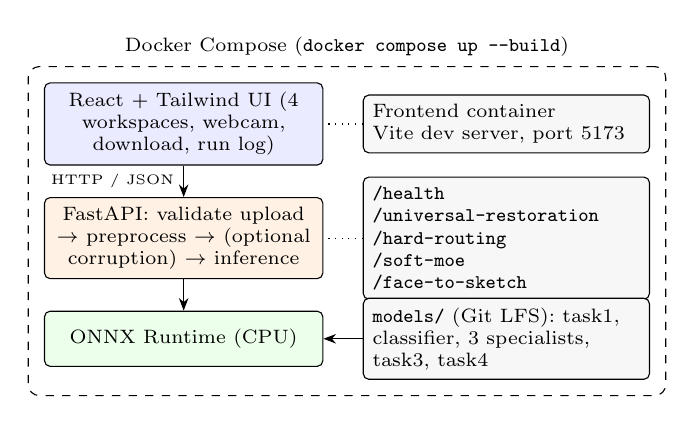
\begin{tikzpicture}[font=\scriptsize, node distance=4mm and 5mm,
  box/.style={draw, rounded corners=2pt, align=center, minimum height=7mm, text width=3.3cm, fill=#1},
  box/.default=white, side/.style={draw, rounded corners=2pt, align=left, text width=3.4cm, fill=gray!6},
  >={Stealth[length=1.6mm]}]
\node[box=blue!8] (ui) {React + Tailwind UI (4 workspaces, webcam, download, run log)};
\node[box=orange!10, below=of ui] (api) {FastAPI: validate upload $\rightarrow$ preprocess $\rightarrow$ (optional corruption) $\rightarrow$ inference};
\node[box=green!8, below=of api] (ort) {ONNX Runtime (CPU)};
\node[side, right=of ui] (fe) {Frontend container\\Vite dev server, port 5173};
\node[side, right=of api] (ep) {\texttt{/health}\\\texttt{/universal-restoration}\\\texttt{/hard-routing}\\\texttt{/soft-moe}\\\texttt{/face-to-sketch}};
\node[side, right=of ort] (m) {\texttt{models/} (Git LFS): task1, classifier, 3 specialists, task3, task4};
\draw[->] (ui) -- node[left, font=\tiny]{HTTP / JSON} (api);
\draw[->] (api) -- (ort);
\draw[->] (m) -- (ort);
\draw[dotted] (fe) -- (ui); \draw[dotted] (ep) -- (api);
\node[draw, dashed, rounded corners, inner sep=2mm, fit=(ui)(api)(ort)(fe)(ep)(m), label={[font=\scriptsize]above:Docker Compose (\texttt{docker compose up --build})}] {};
\end{tikzpicture}
\caption{Application architecture: browser front end, FastAPI back end and ONNX Runtime models, started with one Docker Compose command.}
\label{fig:apparch}
\end{figure}

\subsection{Containerised deployment}
Fig.~\ref{fig:apparch} shows the deployed architecture. The back end (\texttt{python:3.11-slim}, ONNX Runtime) and the front end (\texttt{node:20}, Vite) each have a Dockerfile. \texttt{docker compose up --build} starts both, with the models mounted read-only from \texttt{models/} (stored with Git LFS). The application is then available at \texttt{http://localhost:5173}, with the API documentation at \texttt{http://localhost:8000/docs}. No IDE or manual Python step is needed. CPU inference times observed in the application were 212\,ms (Task 1), 194\,ms (Task 2), 969\,ms (Task 3, four networks) and 54--252\,ms (Task 4). The first request includes model loading.

\subsection{Experiment tracking}
Each notebook logs to one MLflow tracking store, kept on Google Drive (SQLite plus artifact directory), in four experiments (\texttt{Task1-Universal-AE}, \texttt{Task2-Hard-Routing}, \texttt{Task3-Soft-MoE}, \texttt{Task4-Face2Sketch-cGAN}). Each run records:
\begin{itemize}
\item the selected hyperparameters and per-epoch training/validation histories;
\item every Optuna trial as a nested run;
\item test metrics by corruption, severity or style;
\item the best checkpoints, ONNX files, figures and fixed validation samples.
\end{itemize}
The UI is served from Colab and shown in the demonstration video. The Optuna studies are stored as SQLite (Task 1) and as JSON trial logs (Tasks 2--4).

\begin{figure*}[!t]
\centering

\includegraphics[width=0.85\textwidth]{app_stitch_design.png}
\caption{Original Google Stitch design: prompt history (left) and generated \emph{Universal Restoration} workspace with the four-tab structure (right).}
\label{fig:stitch}
\end{figure*}

\begin{figure*}[!t]
\centering
\subfloat[Universal Restoration (salt-and-pepper, medium).]{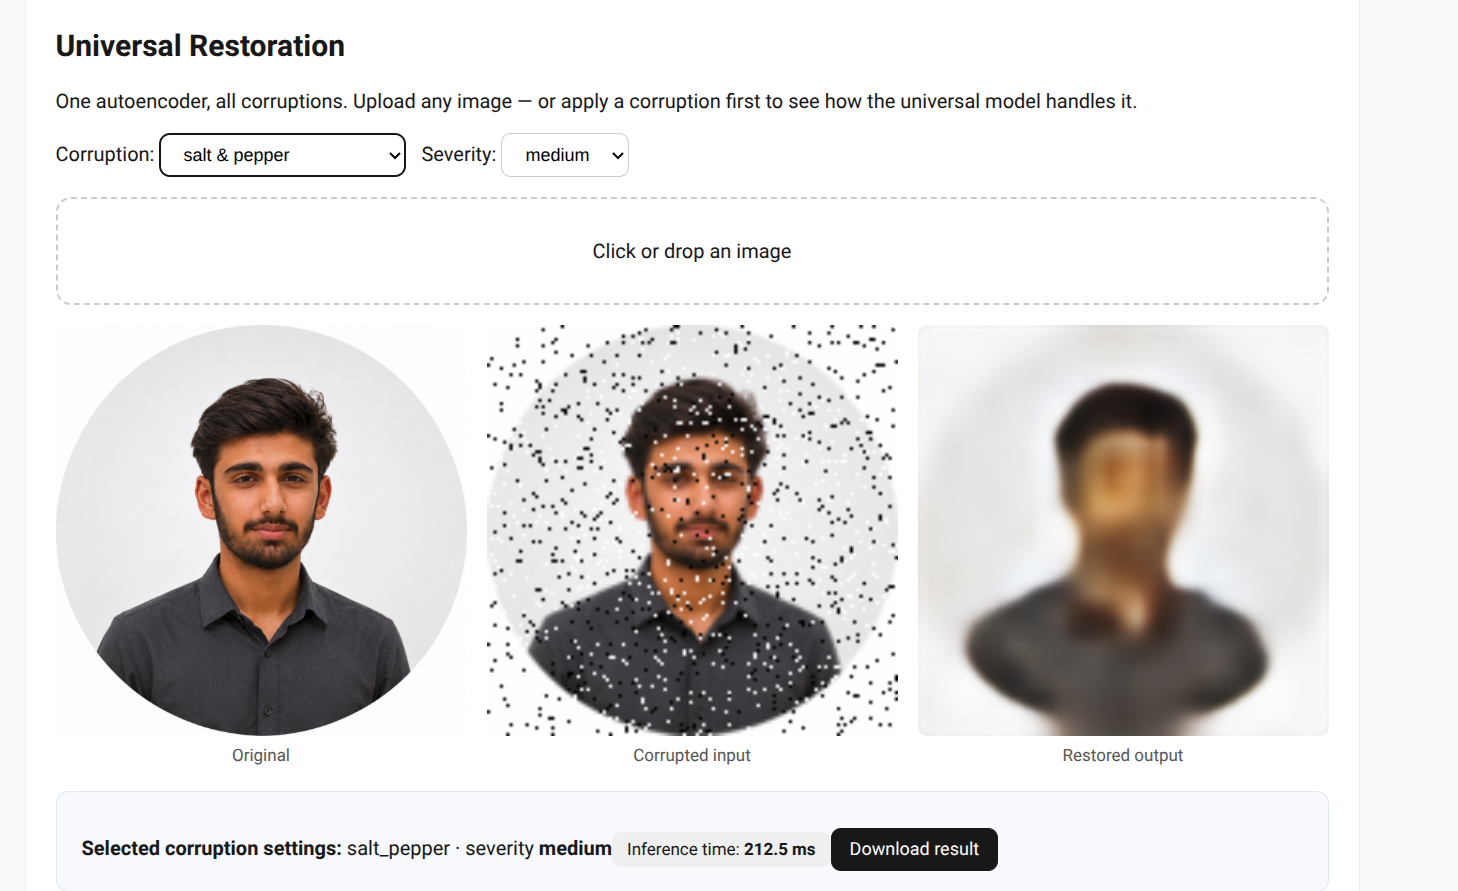
\includegraphics[width=0.49\textwidth]{app_universal.png}}\hfill
\subfloat[Hard-Routed Restoration (blur, medium).]{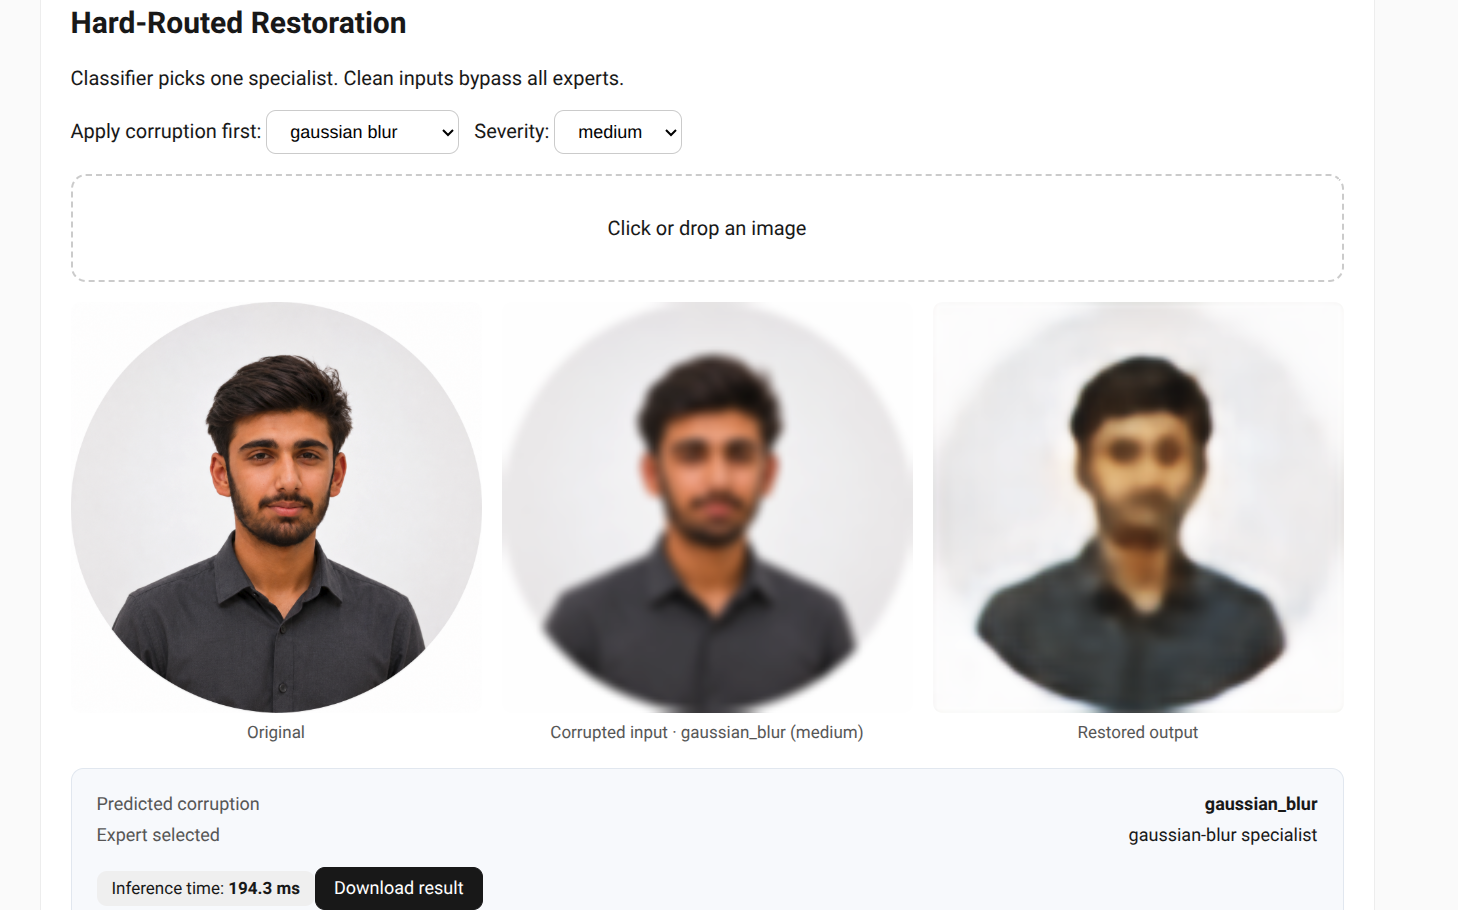
\includegraphics[width=0.49\textwidth]{app_hard_routed.png}}\\
\subfloat[Soft Mixture-of-Experts Restoration.]{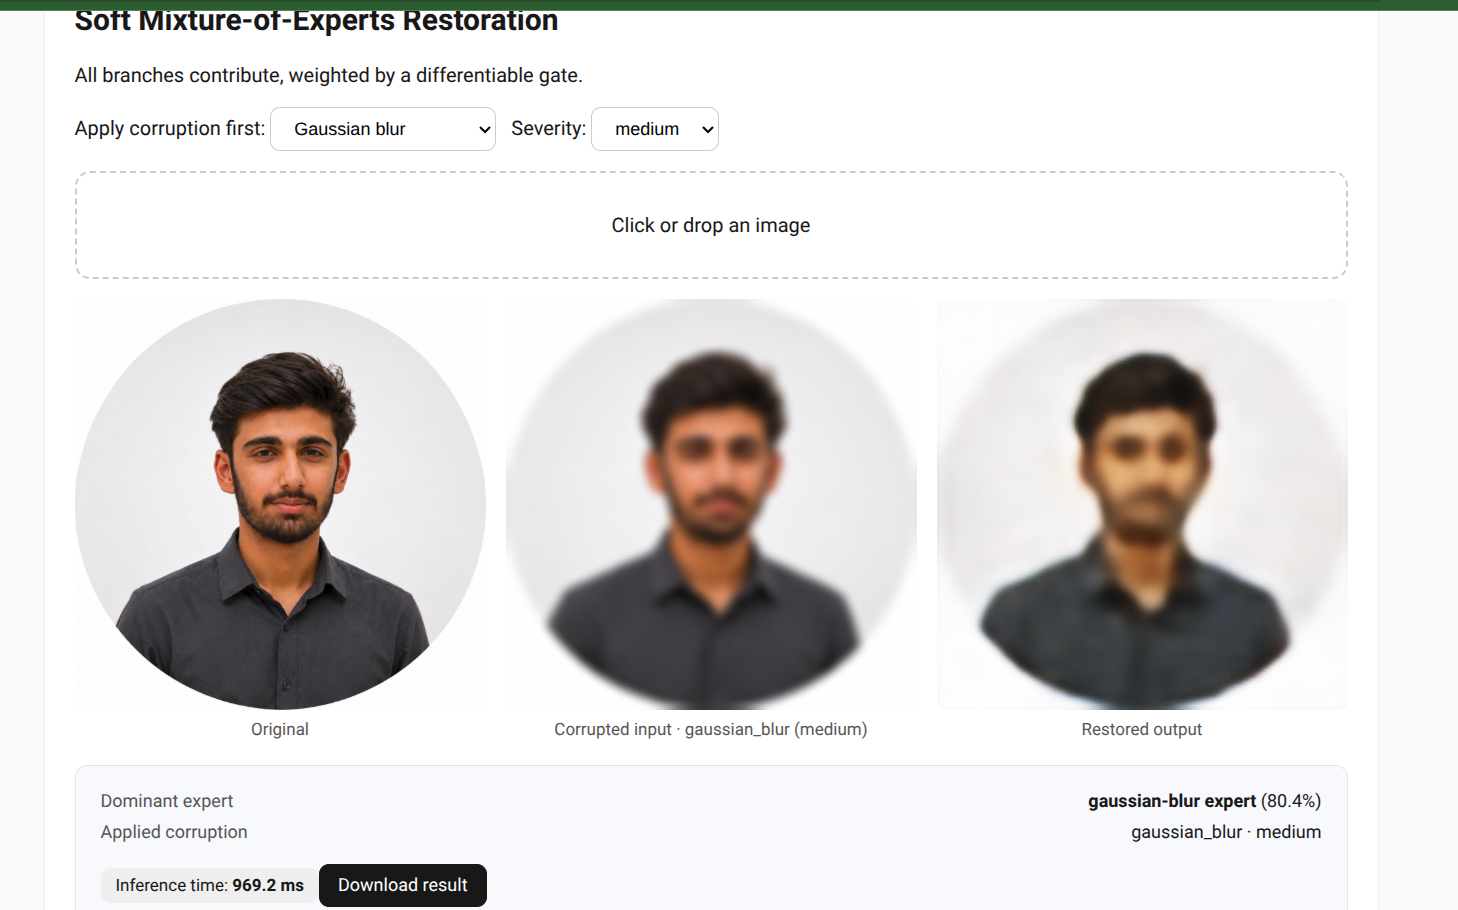
\includegraphics[width=0.49\textwidth]{app_soft_moe.png}}\hfill
\subfloat[Face-to-Sketch Generator, Style 2.]{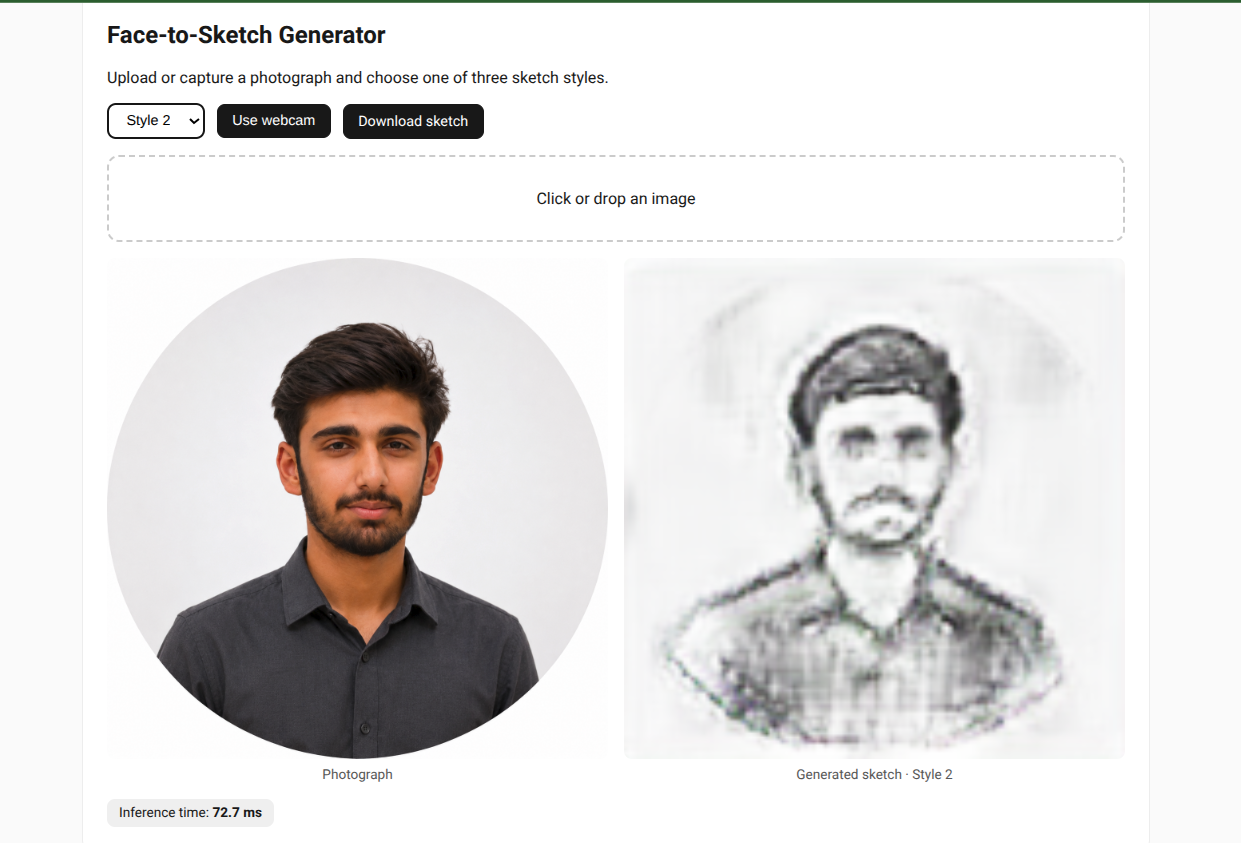
\includegraphics[width=0.49\textwidth]{app_sketch_style2.png}}\\
\subfloat[Style 1.]{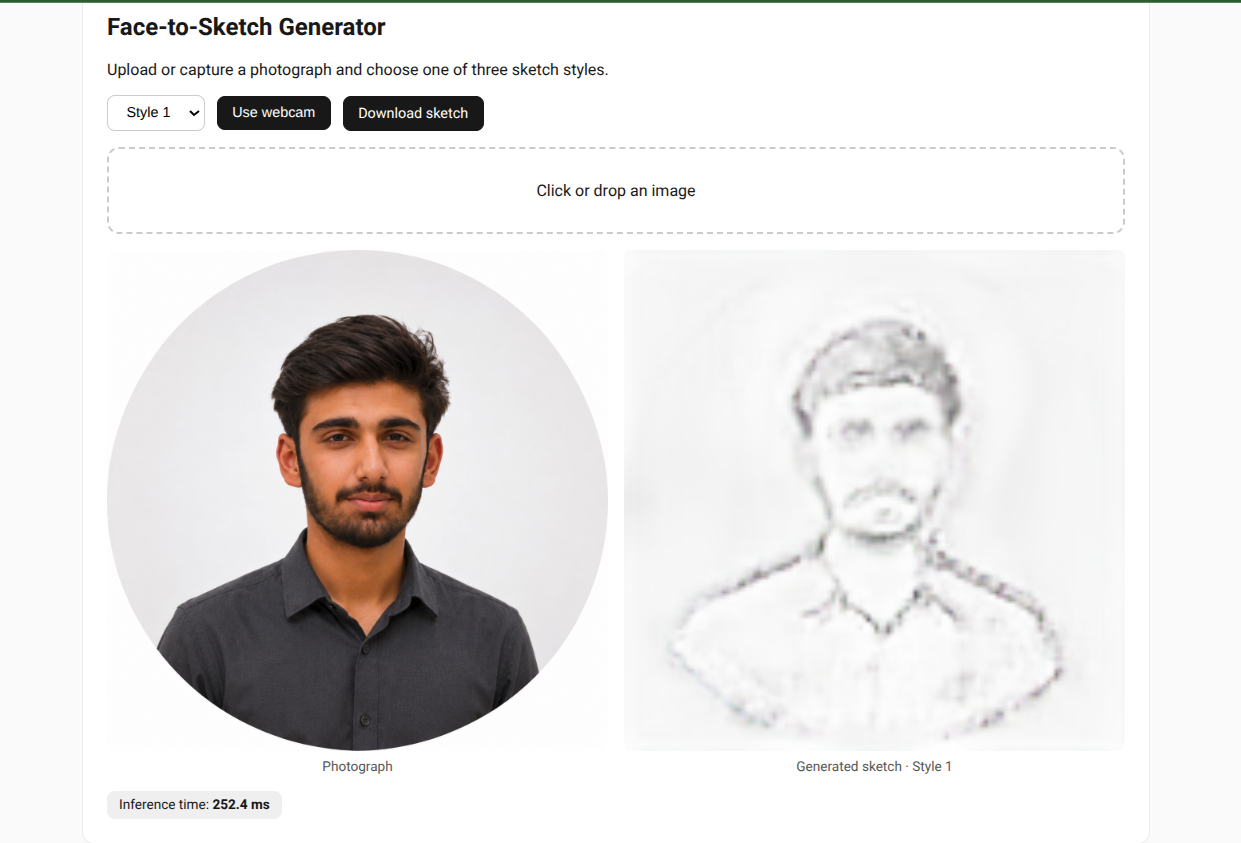
\includegraphics[width=0.32\textwidth]{app_sketch_style1.png}}\hfill
\subfloat[Style 3.]{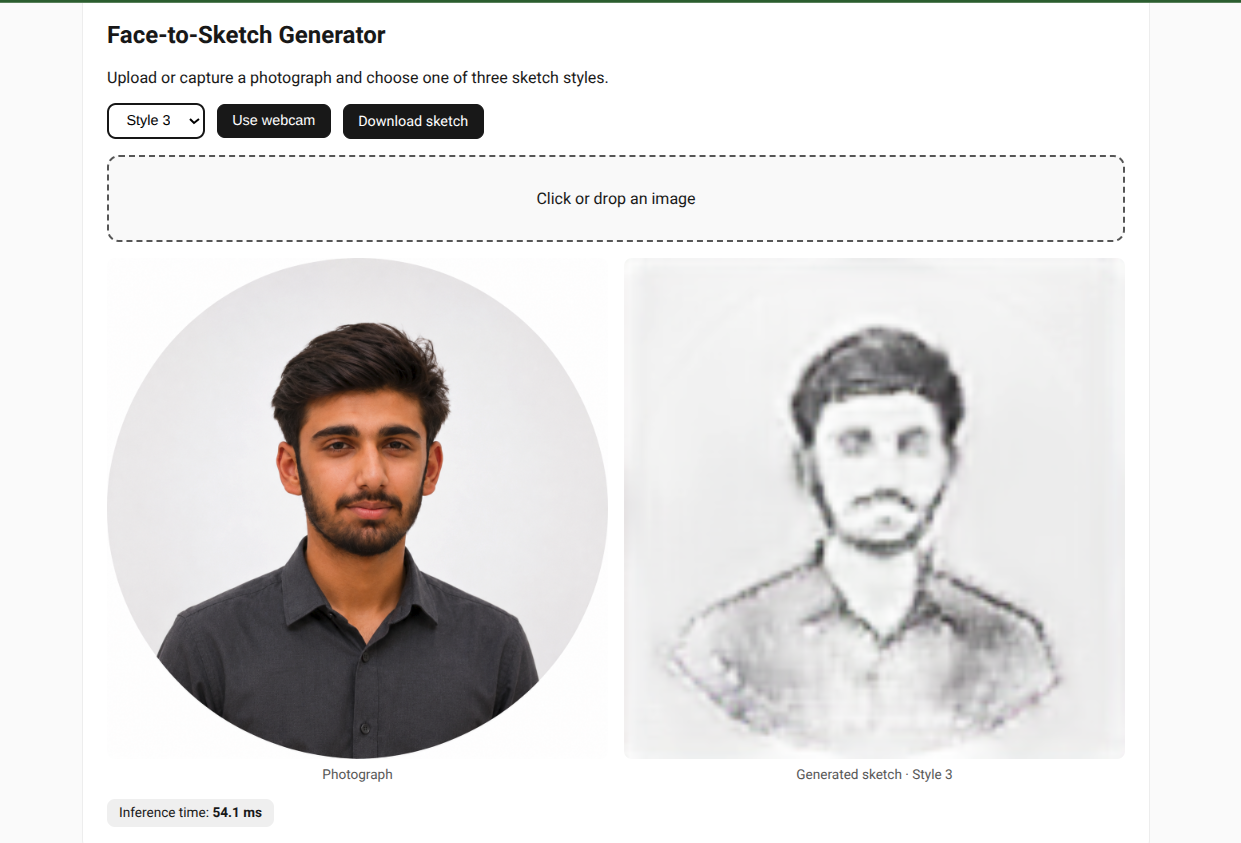
\includegraphics[width=0.32\textwidth]{app_sketch_style3.png}}\hfill
\subfloat[Soft-MoE preview from the notebook.]{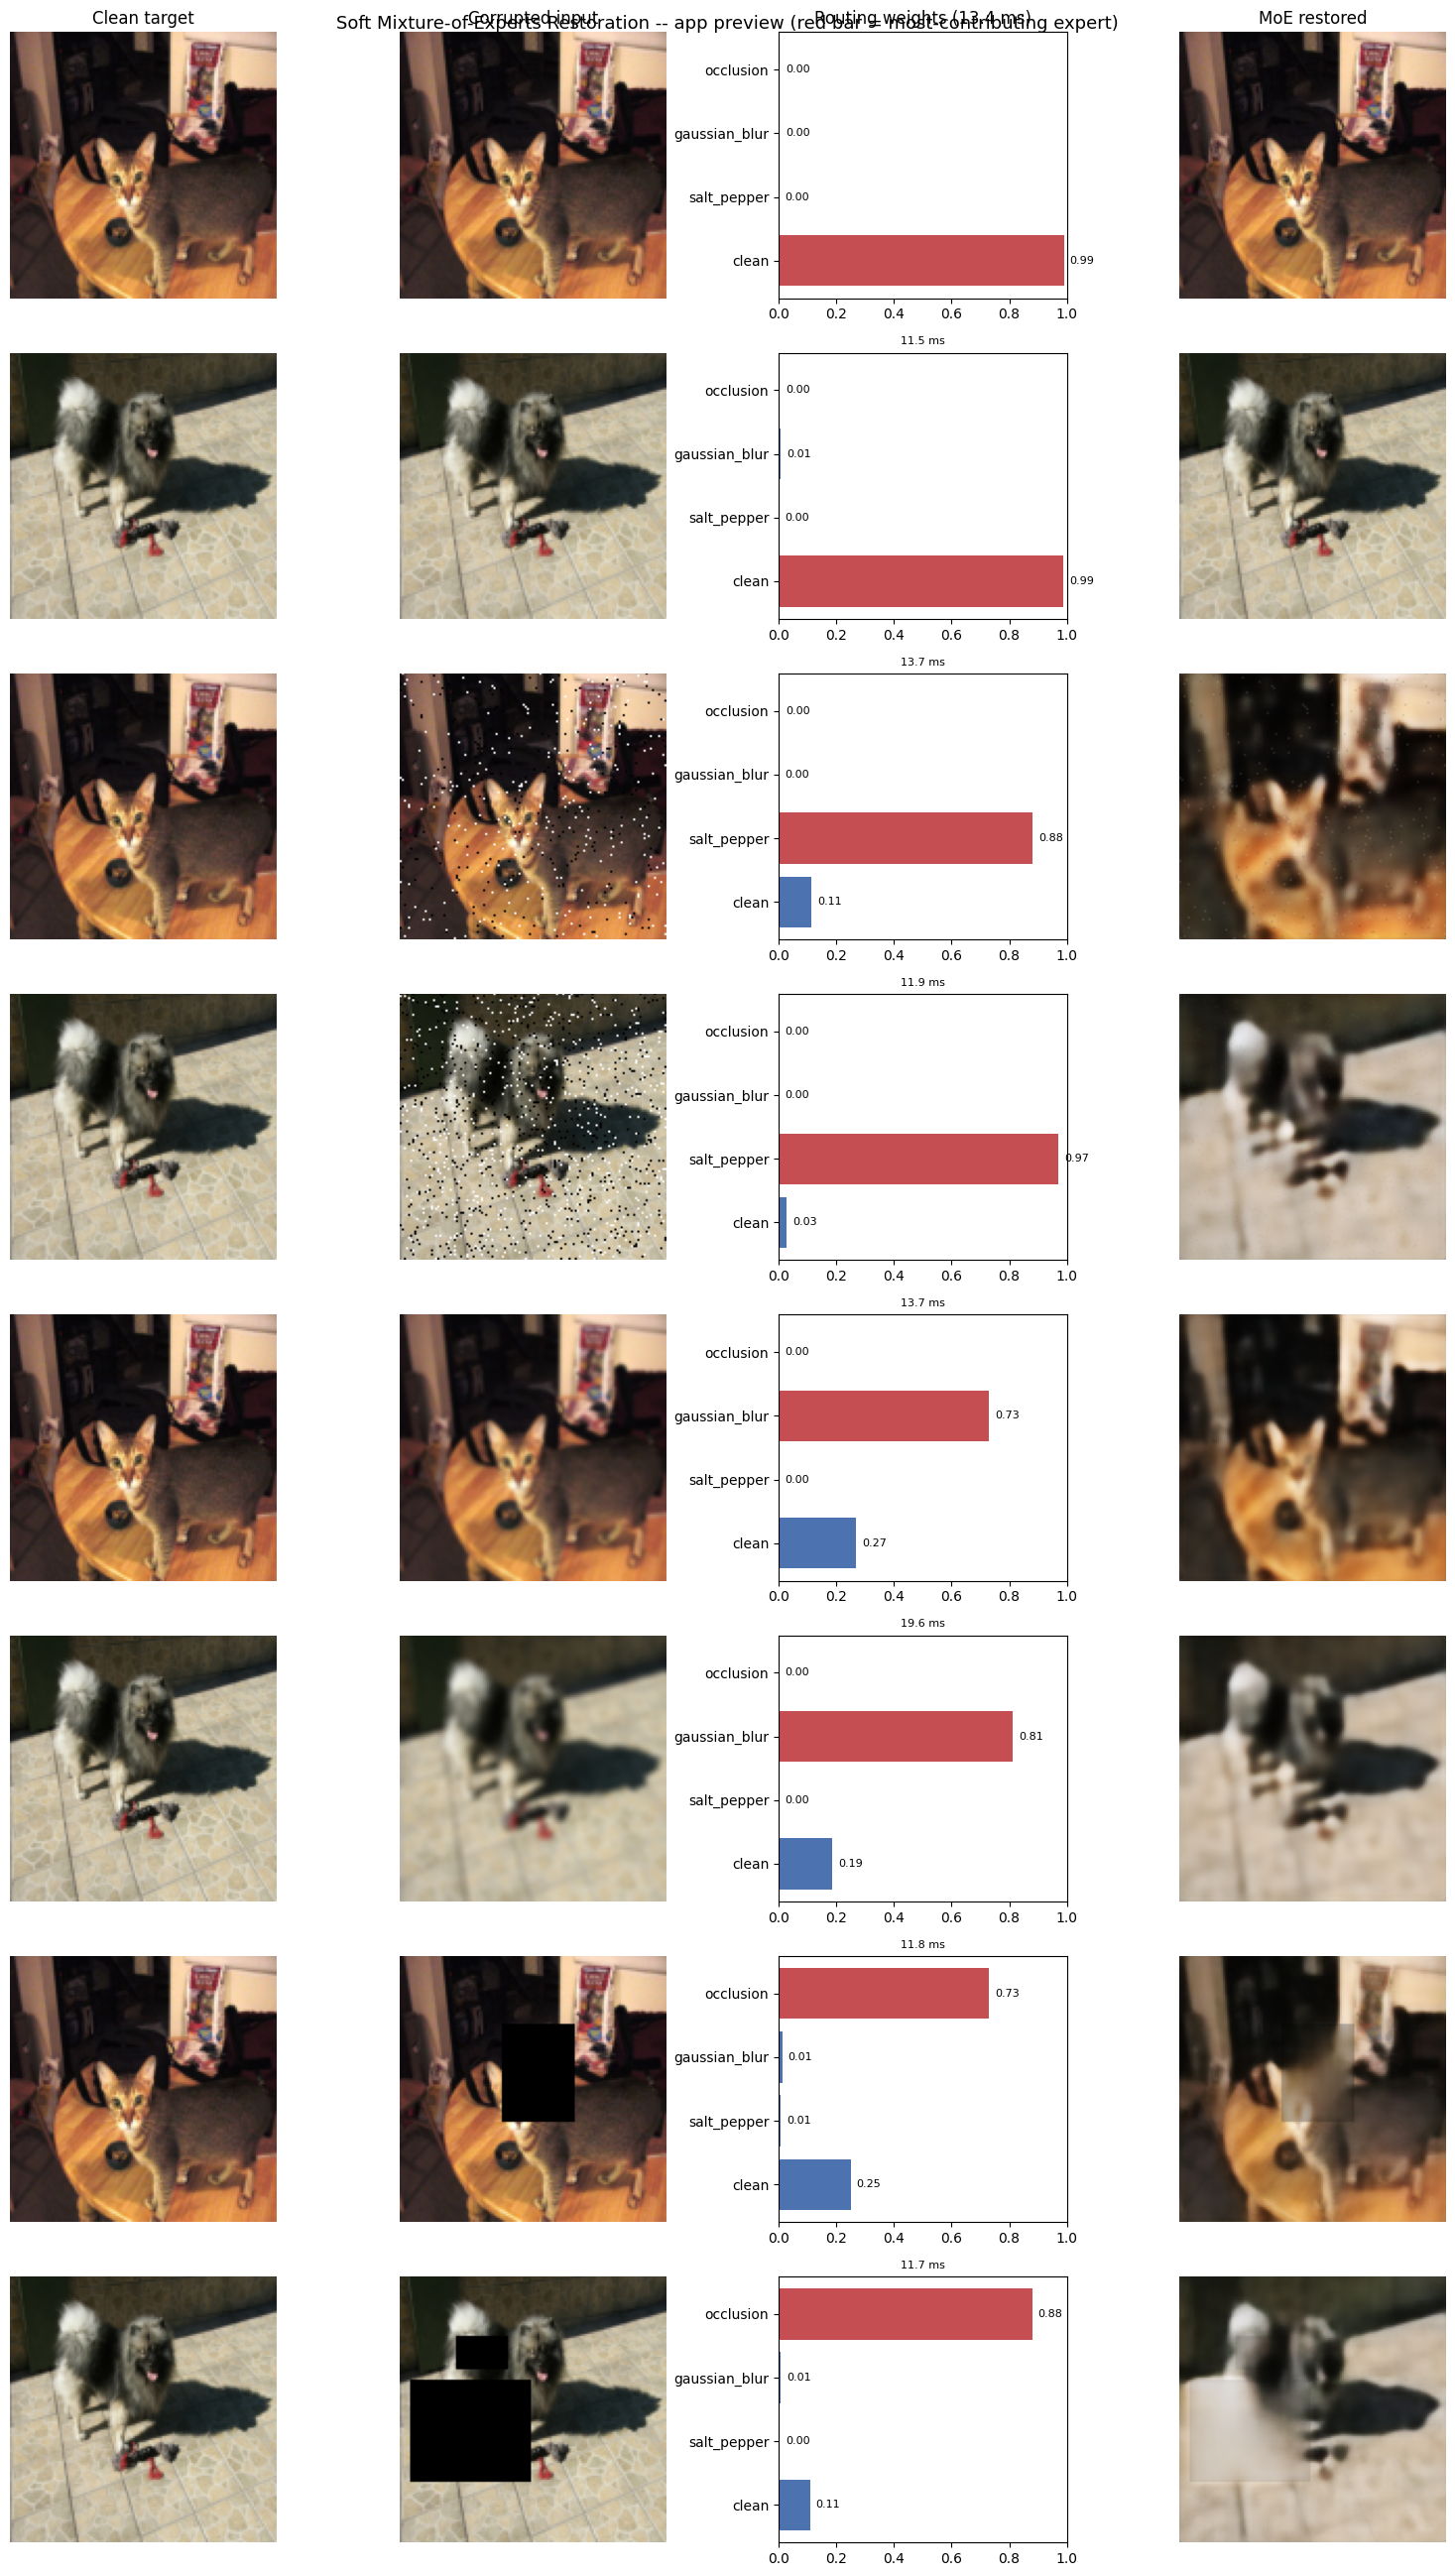
\includegraphics[width=0.18\textwidth]{t3_app_preview.png}}
\caption{Application screenshots of the four workspaces on a previously unseen photograph (input, corruption controls, outputs, predicted corruption/selected expert or dominant expert, inference time and download). The hard-routed and soft-MoE workspaces also render the four class probabilities and the four routing weights as bars below the result card; the same information is shown for test images in Fig.~\ref{fig:t2pipe} and panel~(g).}
\label{fig:app}
\end{figure*}

%=====================================================================
\section{Discussion}
\textbf{Universal vs hard vs soft.} On identical data and manifests, quality improves at each stage: universal (evaluated checkpoint) $\rightarrow$ hard routing ($+0.29$ SSIM on salt-and-pepper and blur) $\rightarrow$ soft MoE (a further $+0.002$ to $+0.11$). The soft system wins because it can \emph{hedge}: mild corruptions keep part of the input through the identity branch instead of being fully re-synthesised by a smoothing autoencoder.

\textbf{Difficulties and how they were resolved.}
\begin{itemize}
\item Blurry outputs were traced to three causes, each fixed with evidence: an MSE objective (replaced by L1+SSIM~\cite{zhao2017loss}), transposed convolutions (replaced by resize-convolution~\cite{odena2016}) and a flattened bottleneck (made spatial).
\item Training that appeared to hang on Colab was Drive I/O, solved by caching the dataset in RAM.
\item Specialists stopped too early because of a noisy quarter-size validation signal. Dedicated full-size validation manifests per corruption, plus a larger budget, fixed it.
\item Overfit sanity checks (memorising eight pairs) and output-diversity checks separated architectural bugs from undertraining.
\item In the GAN, input-only style conditioning was too weak (verified by measuring output differences between styles) and was replaced by per-block FiLM.
\end{itemize}

%=====================================================================
\section{Conclusion, Limitations and Future Work}
\textbf{Task 1.} A blind universal autoencoder with a spatial bottleneck and contrastive FiLM conditioning trains stably (validation SSIM 0.78). The checkpoint available for evaluation is early-epoch (test SSIM 0.40), and retraining with the logged configuration is required to report the trained model's test performance. Future work: identity-preserving skip gating and longer cosine schedules.

\textbf{Task 2.} A balanced-batch classifier (98.3\% accuracy) routes inputs to specialists that restore far better than the evaluated universal model. Its errors are concentrated on mild corruptions misread as clean. Future work: confidence-thresholded fallback to a soft combination.

\textbf{Task 3.} A soft MoE initialised from Task 2 and trained with a batch-level balance loss improves on hard routing for every corrupted condition, without inactive or dominating experts. It costs three expert passes per image. Future work: top-$k$ sparse evaluation and mixed-corruption training.

\textbf{Task 4.} The style-conditioned pix2pix generator produces distinguishable styles (83\% style match) without mode collapse, but loses hair detail. A filename-collision pairing error was discovered in failure analysis. Future work: corrected pairing, perceptual or LPIPS losses and higher resolution.

%=====================================================================
\appendices
\section{AI-Use Disclosure}
\textbf{Claude (Anthropic), through Claude Code}, was used for:
\begin{itemize}
\item reviewing the notebooks against the rubric and adding cells that run on the saved checkpoints, for sample and severity grids, Optuna plots, training curves, failure cases with error maps, ONNX-vs-PyTorch checks, style-confusion and mode-collapse analysis, and MLflow logging;
\item back-end fixes: upload validation and the Task 4 $[-1,1]$ scaling;
\item adding Tailwind CSS;
\item drafting this report and the README.
\end{itemize}
The outputs were verified by executing every notebook end to end on Colab and checking that each reported number appears in the cell outputs. The generated code was checked for undefined names before running. The fixed Task 4 scaling was compared against the raw ONNX output range, and the frontend was confirmed to compile (\texttt{vite build}). All design decisions, training runs and results are the author's. Reused material: the FS2K and Oxford-IIIT Pet datasets, the PyTorch, \texttt{pytorch-msssim}, Optuna, MLflow and ONNX Runtime libraries, and the ideas adapted from AirNet~\cite{li2022airnet} and pix2pix~\cite{isola2017}, as cited.

%=====================================================================
\begin{thebibliography}{99}
\bibitem{akiba2019optuna} T.~Akiba, S.~Sano, T.~Yanase, T.~Ohta, and M.~Koyama, ``Optuna: A next-generation hyperparameter optimization framework,'' in \emph{Proc. 25th ACM SIGKDD Int. Conf. Knowl. Discovery Data Mining}, 2019, pp. 2623--2631.
\bibitem{vincent2010} P.~Vincent, H.~Larochelle, I.~Lajoie, Y.~Bengio, and P.-A. Manzagol, ``Stacked denoising autoencoders: Learning useful representations in a deep network with a local denoising criterion,'' \emph{J. Mach. Learn. Res.}, vol.~11, pp. 3371--3408, 2010.
\bibitem{li2022airnet} B.~Li, X.~Liu, P.~Hu, Z.~Wu, J.~Lv, and X.~Peng, ``All-in-one image restoration for unknown corruption,'' in \emph{Proc. IEEE/CVF Conf. Comput. Vis. Pattern Recognit. (CVPR)}, 2022, pp. 17452--17462.
\bibitem{shazeer2017} N.~Shazeer, A.~Mirhoseini, K.~Maziarz, A.~Davis, Q.~Le, G.~Hinton, and J.~Dean, ``Outrageously large neural networks: The sparsely-gated mixture-of-experts layer,'' in \emph{Proc. Int. Conf. Learn. Represent. (ICLR)}, 2017.
\bibitem{isola2017} P.~Isola, J.-Y. Zhu, T.~Zhou, and A.~A. Efros, ``Image-to-image translation with conditional adversarial networks,'' in \emph{Proc. IEEE Conf. Comput. Vis. Pattern Recognit. (CVPR)}, 2017, pp. 1125--1134.
\bibitem{odena2016} A.~Odena, V.~Dumoulin, and C.~Olah, ``Deconvolution and checkerboard artifacts,'' \emph{Distill}, 2016.
\bibitem{chen2020simclr} T.~Chen, S.~Kornblith, M.~Norouzi, and G.~Hinton, ``A simple framework for contrastive learning of visual representations,'' in \emph{Proc. Int. Conf. Mach. Learn. (ICML)}, 2020, pp. 1597--1607.
\bibitem{perez2018film} E.~Perez, F.~Strub, H.~de~Vries, V.~Dumoulin, and A.~Courville, ``FiLM: Visual reasoning with a general conditioning layer,'' in \emph{Proc. AAAI Conf. Artif. Intell.}, 2018.
\bibitem{pathak2016} D.~Pathak, P.~Kr\"ahenb\"uhl, J.~Donahue, T.~Darrell, and A.~A. Efros, ``Context encoders: Feature learning by inpainting,'' in \emph{Proc. IEEE Conf. Comput. Vis. Pattern Recognit. (CVPR)}, 2016, pp. 2536--2544.
\bibitem{wang2004ssim} Z.~Wang, A.~C. Bovik, H.~R. Sheikh, and E.~P. Simoncelli, ``Image quality assessment: From error visibility to structural similarity,'' \emph{IEEE Trans. Image Process.}, vol.~13, no.~4, pp. 600--612, 2004.
\bibitem{zhao2017loss} H.~Zhao, O.~Gallo, I.~Frosio, and J.~Kautz, ``Loss functions for image restoration with neural networks,'' \emph{IEEE Trans. Comput. Imaging}, vol.~3, no.~1, pp. 47--57, 2017.
\bibitem{johnson2016perceptual} J.~Johnson, A.~Alahi, and L.~Fei-Fei, ``Perceptual losses for real-time style transfer and super-resolution,'' in \emph{Proc. Eur. Conf. Comput. Vis. (ECCV)}, 2016, pp. 694--711.
\bibitem{ronneberger2015unet} O.~Ronneberger, P.~Fischer, and T.~Brox, ``U-Net: Convolutional networks for biomedical image segmentation,'' in \emph{Proc. MICCAI}, 2015, pp. 234--241.
\bibitem{fedus2022switch} W.~Fedus, B.~Zoph, and N.~Shazeer, ``Switch transformers: Scaling to trillion parameter models with simple and efficient sparsity,'' \emph{J. Mach. Learn. Res.}, vol.~23, no.~120, pp. 1--39, 2022.
\bibitem{jacobs1991} R.~A. Jacobs, M.~I. Jordan, S.~J. Nowlan, and G.~E. Hinton, ``Adaptive mixtures of local experts,'' \emph{Neural Comput.}, vol.~3, no.~1, pp. 79--87, 1991.
\bibitem{puigcerver2024soft} J.~Puigcerver, C.~Riquelme, B.~Mustafa, and N.~Houlsby, ``From sparse to soft mixtures of experts,'' in \emph{Proc. Int. Conf. Learn. Represent. (ICLR)}, 2024.
\bibitem{he2020moco} K.~He, H.~Fan, Y.~Wu, S.~Xie, and R.~Girshick, ``Momentum contrast for unsupervised visual representation learning,'' in \emph{Proc. IEEE/CVF Conf. Comput. Vis. Pattern Recognit. (CVPR)}, 2020, pp. 9729--9738.
\bibitem{goodfellow2014gan} I.~Goodfellow \emph{et al.}, ``Generative adversarial nets,'' in \emph{Adv. Neural Inf. Process. Syst. (NeurIPS)}, 2014, pp. 2672--2680.
\bibitem{mirza2014cgan} M.~Mirza and S.~Osindero, ``Conditional generative adversarial nets,'' arXiv:1411.1784, 2014.
\bibitem{ulyanov2016instance} D.~Ulyanov, A.~Vedaldi, and V.~Lempitsky, ``Instance normalization: The missing ingredient for fast stylization,'' arXiv:1607.08022, 2016.
\bibitem{wu2018gn} Y.~Wu and K.~He, ``Group normalization,'' in \emph{Proc. Eur. Conf. Comput. Vis. (ECCV)}, 2018, pp. 3--19.
\bibitem{bergstra2011tpe} J.~Bergstra, R.~Bardenet, Y.~Bengio, and B.~K\'egl, ``Algorithms for hyper-parameter optimization,'' in \emph{Adv. Neural Inf. Process. Syst. (NeurIPS)}, 2011, pp. 2546--2554.
\bibitem{zaharia2018mlflow} M.~Zaharia \emph{et al.}, ``Accelerating the machine learning lifecycle with MLflow,'' \emph{IEEE Data Eng. Bull.}, vol.~41, no.~4, pp. 39--45, 2018.
\bibitem{onnxruntime} ONNX Runtime developers, ``ONNX Runtime,'' 2021. [Online]. Available: \url{https://onnxruntime.ai}
\bibitem{parkhi2012pets} O.~M. Parkhi, A.~Vedaldi, A.~Zisserman, and C.~V. Jawahar, ``Cats and dogs,'' in \emph{Proc. IEEE Conf. Comput. Vis. Pattern Recognit. (CVPR)}, 2012, pp. 3498--3505.
\bibitem{fan2022fs2k} D.-P. Fan, Z.~Huang, P.~Zheng, H.~Liu, X.~Qin, and L.~Van~Gool, ``Facial-sketch synthesis: A new challenge,'' \emph{Mach. Intell. Res.}, vol.~19, no.~4, pp. 257--287, 2022.
\end{thebibliography}

\end{document}
